\documentclass[11pt,a4paper]{article}

\usepackage[utf8]{inputenc}
\usepackage[T1]{fontenc}
\usepackage[english]{babel}
\usepackage{lmodern}
\usepackage{microtype}
\usepackage[a4paper,margin=2.5cm]{geometry}
\usepackage{amsmath,amssymb,amsfonts,bm,mathtools}
\usepackage{amsthm}
\usepackage{booktabs,array}
\usepackage{graphicx}
\usepackage{float}
\usepackage[section]{placeins}
\usepackage{subcaption}
\usepackage{pgfplots}
\usepgfplotslibrary{groupplots}
\pgfplotsset{compat=1.18}
\usepackage{xcolor,xurl}
\usepackage[colorlinks=true,
  linkcolor=blue,
  citecolor=blue,
  urlcolor=blue,
  pdfborder={0 0 0},
  pdftitle={Relational Capacity Dynamics, RFG, RFG-R, and the Covariant KGB Realization with LCDM Reference Posterior and Bayesian Evidence},
  pdfauthor={Martin Petrásek},
  pdfsubject={Relational Capacity Dynamics, Relational Foliation Gravity, and a covariant KGB realization},
  pdfkeywords={relational capacity, preferred foliation, kinetic gravity braiding, modified gravity, cosmology, CMB likelihood, gravitational waves, standard sirens}]{hyperref}
\usepackage{enumitem}
\usepackage{physics}
\setlength{\parindent}{1.1em}
\setlength{\parskip}{0.3em}
\setlength{\emergencystretch}{3em}
\renewcommand{\arraystretch}{1.15}

\newtheorem{axiom}{Axiom}[section]
\newtheorem{definition}[axiom]{Definition}
\newtheorem{theorem}[axiom]{Theorem}
\newtheorem{lemma}[axiom]{Lemma}
\newtheorem{proposition}[axiom]{Proposition}
\newtheorem{corollary}[axiom]{Corollary}
\newtheorem{remark}[axiom]{Remark}
\newtheorem{openproblem}[axiom]{Open problem}

\newcommand{\C}{\mathcal{C}}
\newcommand{\Cs}{\mathcal{C}_\star}
\newcommand{\Jc}{\mathbf{J}_{\mathcal{C}}}
\newcommand{\Sc}{\mathcal{S}_{\mathcal{C}}}
\newcommand{\Ac}{\mathbf{A}_{\mathcal{C}}}
\renewcommand{\dd}{\mathrm{d}}
\newcommand{\e}{\mathrm{e}}
\newcommand{\Lag}{\mathcal{L}}
\newcommand{\Ham}{\mathcal{H}}
\newcommand{\RCD}{\mathrm{RCD}}
\newcommand{\RFG}{\mathrm{RFG}}
\newcommand{\rhoC}{\rho_{\mathcal{C}}}
\newcommand{\kC}{\kappa_{\mathcal{C}}}
\newcommand{\mpl}{M_{\rm Pl}}
\newcommand{\threeR}{{}^{(3)}R}
% Permanent public source location; the complete local bundle is nested below.
\newcommand{\RFGRepoURL}{https://github.com/MartinPetrasek123/MartinPetrasek123}
\newcommand{\RFGRepoRevision}{v1.6.1}
\newcommand{\RFGRepoPath}[1]{\href{\RFGRepoURL/blob/\RFGRepoRevision/r-universe-complete-chain/rfg-r-completion/r\_universe\_completion/#1}{\texttt{#1}}}
\newcommand{\RFGRepoNamed}[2]{\href{\RFGRepoURL/blob/\RFGRepoRevision/r-universe-complete-chain/rfg-r-completion/r\_universe\_completion/#1}{\texttt{#2}}}
\newcommand{\RFGLocalPath}[1]{\texttt{r\_universe\_completion/#1}}
% Public reproducibility record for the covariant KGB realization.
\newcommand{\KGBRepoURL}{https://github.com/MartinPetrasek123/MartinPetrasek123}
\newcommand{\KGBRepoRevision}{v1.6.1}
\newcommand{\KGBRepoPath}[1]{\href{\KGBRepoURL/blob/\KGBRepoRevision/r-universe-global-kgb-completion/#1}{\texttt{#1}}}
\newcommand{\KGBRepoNamed}[2]{\href{\KGBRepoURL/blob/\KGBRepoRevision/r-universe-global-kgb-completion/#1}{\texttt{#2}}}
\newcommand{\KGBRepoRelease}{\href{\KGBRepoURL/tree/\KGBRepoRevision}{\texttt{\KGBRepoRevision}}}
% note: keep single outer brace group for safe use inside \bigl( ... \bigr)
\newcommand{\Boxed}[1]{\boxed{\displaystyle #1}}
\newcommand{\doi}[1]{\href{https://doi.org/#1}{\textcolor{blue}{doi:#1}}}

\title{\textbf{Relational Capacity Dynamics, Relational Foliation Gravity, and RFG-R}\\[0.4em]
\large Full proof version: original branch, regular effective completion,\\ local-GR matching, an extended-EFT likelihood boundary, an exact KGB posterior,\\ a local \(\Lambda\)CDM reference posterior, and production Bayesian evidence}

\author{Martin Petr\'{a}sek\\[0.3em]
\small ORCID: \href{https://orcid.org/0009-0007-4512-9528}{0009-0007-4512-9528}\\[0.2em]
\small Institute for Resonant Synthesis and Field Physics (IRSFP)\\
\small Prague, Czech Republic\\
\small \href{mailto:martin.petrasek@irsfp.org}{martin.petrasek@irsfp.org}}

\date{August 2026}

\begin{document}

\maketitle

\begin{abstract}
We present a unified theoretical framework that begins with a non-geometric macroscopic scalar theory---Relational Capacity Dynamics (RCD)---and constructs a covariant preferred-foliation completion---Relational Foliation Gravity (RFG). The primitive variable of the scalar sector is a strictly positive relational-capacity field \(\C(\tau,\mathbf{x})\). We supply the complete ontology, dimensional structure, conservative action, full variational derivation, Hamiltonian formulation, Noether identities with explicit local currents, finite-response transport, emergent physical-time map, and linear stability analysis. The scalar sector is ghost-free for \(\rhoC>0\), gradient-stable for \(\kC>0\), and strictly hyperbolic with characteristic speed \(c_{\mathcal{C}}=\sqrt{\kC/\rhoC}\).

The original covariant completion is defined by a metric--khronon action whose two free functions are uniquely reconstructed from a conserved relational-capacity law and the requirement of luminal tensor propagation. The resulting homogeneous cosmology yields the closed algebraic equation
\[
E^2=\Omega_{m0}a^{-3}+\Omega_{r0}a^{-4}+\Omega_{R0}E^{2-\theta},
\]
together with a proof of existence and uniqueness of the expanding branch, exact expressions for the logarithmic Hubble derivative, deceleration parameter, effective equation of state, acceleration--capacity identity, early- and late-time asymptotics, and a falsifiable standard-siren distance relation with \(c_T=1\).

The RFG-R extension introduced here is a separate, explicitly defined low-energy multiscale EFT. It regularizes the \(X\to0\) action, preserves the original homogeneous branch to controlled order, and matches exactly to GR in a specified local-curvature domain. It consequently gives a definite local PPN prediction. Its regularized action, potential reconstruction, numerical validation, and Cassini likelihood factor are supplied as executable source files. For RFG-R coupled to one minimally coupled canonical scalar, the sourced lapse--shift constraints and the reduced quadratic action are also evaluated exactly, including the GR normalization check \(K=6\), \(c_s^2=1\). The action is mapped exactly into the extended EFT basis; the map forces a nonzero \(\bar m_5\,\delta{}^{(3)}R\,\delta K\) operator that is absent from the public stock H-EFTCAMB input basis~\cite{EFTCAMB}. The complete \emph{pure-gravity} extended-EFT scalar action is degenerate. The sourced photon--baryon--CDM--neutrino action, untruncated kinetic hierarchy, and the remaining spatial metric equations are derived directly from the same action; their exact DAE closure has a finite-wavenumber curvature-constraint singularity on the published reference branch. A distinct, background-null RFG-R\(\Xi\) action is then derived directly from the preferred-foliation invariants \({}^{(3)}R+\sigma_{ij}\sigma^{ij}\): it removes that detected zero on the stated finite DAE grid while leaving the R-Universe Friedmann branch and \(c_T=1\) unchanged. An external GR/CAMB spectrum and Planck low-ell+lensing reference has been executed only to validate the data interface. Neither RFG-R nor RFG-R\(\Xi\) has an executed cosmological data likelihood.

For the same R-Universe background law, this paper also supplies an explicitly declared covariant Kinetic Gravity Braiding (KGB) realization. Its action reconstruction, global scalar-stability tests, and native photon--baryon--CDM--neutrino H--EFTCAMB evolution are executable. At one fully declared parameter point, the official Planck 2018 TTTEEE, low-\(\ell\), and lensing likelihood objects give \(-2\ln\mathcal L=1210.1599180\). An executed fixed-input extension combines Planck with Pantheon+, DESI DR2 BAO, and chronometers; at the selected matched point, its KGB-minus-\(\Lambda\)CDM conditional sum is \(-2.5637653\). The same KGB point has a direct native \(f\sigma_8\) audit and a local screening gate. Four independent exact chains also yield a converged Planck--Pantheon+--DESI DR2 BAO--chronometer posterior for this stated KGB action after the declared 25\% per-chain burn-in: the largest rank-normalized folded split-\(\hat R\) is \(1.0066\), and the minimum bulk and tail ESS values are \(690.2\) and \(1214.6\). A separate local \(\Lambda\)CDM control posterior using the same stated CMB and late-time probe family reaches four independent 12,000-sample chains and recovers a standard benchmark region, with \(\Omega_{m0}=0.2971\pm0.0035\), \(\omega_b=0.02240\pm0.00012\), \(n_s=0.9682\pm0.0033\), \(\tau=0.0386\pm0.0086\), \(A_{\rm Planck}=0.9993\pm0.0025\), and a best sampled \(\chi^2=2454.7832\). This control run supports the data-interface and calibration status of the R-Universe analysis, but it is not imposed as a target surface: R-Universe KGB need not copy the individual \(\Lambda\)CDM parameter values. Finally, dedicated dynamic nested-sampling evidence calculations over the explicitly declared Cobaya priors give
\(\log Z_{\rm KGB}=-1335.5996905\pm2.8042019\) and
\(\log Z_{\Lambda{\rm CDM}}=-1291.3199169\pm2.8135177\), hence
\(\Delta\log Z=\log Z_{\rm KGB}-\log Z_{\Lambda{\rm CDM}}=-44.2797735\).
Thus the production marginal likelihood favors the local \(\Lambda\)CDM reference for this exact probe set and prior volume, even though the fixed-input conditional profile is slightly better for the selected KGB point. The KGB action remains a physical R-Universe replacement candidate with a completed posterior and evidence audit, but final empirical replacement is not asserted; the RSD compilation is still not a survey likelihood.
\end{abstract}

\bigskip
\noindent\textbf{Keywords:}
Relational Capacity Dynamics (RCD);
Relational Foliation Gravity (RFG);
emergent time;
relational capacity;
preferred foliation;
scalar field theory;
modified gravity;
Hamiltonian formulation;
Noether currents;
hyperbolic field equations;
cosmology;
gravitational waves;
standard sirens;
Kinetic Gravity Braiding;
CMB likelihood.

\newpage
\section{Introduction}

A fundamental theory must specify its dynamical variables, symmetries, action, variational equations, physical degrees of freedom, initial-value structure, and falsification conditions. A background equation alone is not sufficient. The purpose of this manuscript is to assemble the mathematically derived RCD and RFG layers together with a deliberately explicit, regular low-energy extension, RFG-R. The distinction is essential: RFG-R is a model completion and matching prescription, not a retroactive theorem about the original singular RFG branch.

We distinguish three logically separate statements that must not be conflated:

\begin{enumerate}[label=(\roman*)]
\item \textbf{Mathematical definition:} the action and its variational problem are specified.
\item \textbf{Internal viability:} all propagating modes must be ghost-free, gradient-stable, and compatible with a well-posed initial-value problem.
\item \textbf{Empirical viability:} cosmological, Solar-System, binary-pulsar, gravitational-wave and laboratory data must be fitted with a reproducible likelihood.
\end{enumerate}

The original calculation completes item~(i) for the scalar macroscopic sector and for the homogeneous and tensor sectors of the preferred-foliation theory. RFG-R additionally defines a regular action and an exact local-GR domain, but it does not make the original scalar perturbation degeneracy disappear. Preferred-foliation and ADM-based constructions provide the broader mathematical context~\cite{ADM,JacobsonMattingly,Horava,BlasPujolasSibiryakov}. Its ADM action is now mapped to the extended EFT basis~\cite{ExtendedEFTMap}; that mapping identifies the operator which a full 3+1 Einstein--Boltzmann implementation must retain, rather than replacing the perturbation theory by a background-only surrogate.

The final empirical section adds an action-faithful data execution without rewriting the RFG-R result. It gives a covariant KGB realization of the same R-Universe background law, reconstructs its four scalar functions, and evolves that action through the reparametrized-Horndeski interface of H--EFTCAMB. This is an additional realization within the present manuscript, not an identification of the KGB action with RFG-R: the fixed-point likelihood, conditional multi-probe record, and exact posterior reported below apply to the stated KGB action alone.

The logical hierarchy followed throughout is
\[
\text{ontology}\;\longrightarrow\;
\text{state space}\;\longrightarrow\;
\text{action}\;\longrightarrow\;
\text{equations}\;\longrightarrow\;
\text{stability}\;\longrightarrow\;
\text{observables}.
\]

\begin{table}[H]
\centering
\caption{Scope comparison for the constructions in this paper. ``Defined'' is not a data fit, and an entry for a particular sector does not imply health of every perturbative sector.}
\label{tab:comparison}
\resizebox{\textwidth}{!}{%
\begin{tabular}{@{}lcccc@{}}
\toprule
Framework & Scalar status & Tensor speed & Effective \(w_R(a)\) & Analytic background closure \\
\midrule
\(\Lambda\)CDM & N/A & \(c_T=1\) & \(w=-1\) (const.) & Yes \\
Quintessence / K-essence & Conditional (\(c_s^2>0\)) & \(c_T=1\) & Potential-dependent & Selected potentials only \\
Horndeski / DHOST & After cleaning & Generally \(c_T(z)\neq1\) & Dynamical & Varies \\
\textbf{RCD / original RFG} & RCD stable; RFG FLRW scalar degeneracy & \(c_T=1\) (exact) & \(w_R(a)>-1\) (derived) & Yes (Eq.~\eqref{eq:background}) \\
\textbf{RFG-R EFT} & Exact finite multi-fluid constraint core; kinetic hierarchy & \(c_T=1\) on FLRW & Regularized branch & Yes (Eq.~\eqref{eq:RFGR-background}) \\
\textbf{Covariant KGB R-Universe} & Positive \(Q_s,c_s^2\) on stated scan & \(c_T=1\) (exact) & Reconstructed & Yes (Eq.~\eqref{eq:KGB-background}) \\
\bottomrule
\end{tabular}%
}
\end{table}

\begin{table}[H]
\centering
\caption{Closure ledger used throughout the manuscript. The table prevents a common failure mode in speculative theory papers: treating a selected branch, reconstruction condition, or calculational target as if it were already a theorem.}
\label{tab:closure-ledger}
\resizebox{\textwidth}{!}{%
\begin{tabular}{@{}p{0.23\textwidth}p{0.25\textwidth}p{0.42\textwidth}@{}}
\toprule
Layer & Status in this manuscript & Precise content \\
\midrule
RCD scalar ontology and action & Closed classical sector & \(\C>0\), \(\varphi=\ln(\C/\Cs)\), action, Euler--Lagrange equation, Hamiltonian, Noether currents, linear hyperbolicity. \\
Finite-response transport & Closed once constitutive data are fixed & Maxwell--Cattaneo relaxation law and entropy-production condition; not a fundamental microscopic derivation. \\
RCD--RFG identification & Branch postulate & The map from \(\C\) to the homogeneous \(X=K/(3H_0)\) branch is imposed through the capacity-scaling law, not yet derived from a common microscopic action. \\
RFG homogeneous background & Derived after branch postulate & \(Q(X)\), \(V(X)\), Friedmann constraint, uniqueness of \(E(a)\), \(w_R(a)\), \(q(a)\), and asymptotic limits. \\
RFG tensor sector & Derived within the action & \(Q_T\), \(c_T=1\), no tensor ghost on the branch, and the standard-siren amplitude ratio. \\
RFG pure-gravity FLRW scalar reduction & Computed & The lapse and scalar shift are solved algebraically; the exact reduced density is \(L_{\rm red}=A\zeta\dot\zeta+B\zeta^2\), with no \(\dot\zeta^2\) term. After integration by parts, \(S_{\rm red}^{(2)}\) is algebraic in time. \\
RFG full scalar constraints with matter & Open completion gate & The metric Legendre rank and the local \({\cal C}\)--\({\cal C}\) bracket are explicit. The global kernel, boundary-condition dependence, complete constraint classification, and matter-coupled scalar reduction remain open before a final degree-of-freedom statement can be claimed. \\
RFG-R local gravitational domain & Defined EFT matching sector & A smooth Weyl-invariant switch makes the local action and all its variations exactly GR; this yields \(\gamma=\beta=1\), \(\alpha_1=\alpha_2=0\) wherever the switch is constant. \\
RFG-R canonical scalar & Computed reference-sector reduction & For one minimally coupled canonical scalar in comoving gauge, the sourced lapse--shift Hessian, its determinant, and the exact Schur-complement action are derived. The GR stiff-field limit and a regular reference branch pass the stated kinetic and low-gradient checks. \\
\bottomrule
\end{tabular}%
}
\end{table}

\begin{table}[H]
\centering
\caption{Closure ledger used throughout the manuscript (continued).}
\label{tab:closure-ledger-continued}
\resizebox{\textwidth}{!}{%
\begin{tabular}{@{}p{0.23\textwidth}p{0.25\textwidth}p{0.42\textwidth}@{}}
\toprule
Layer & Status in this manuscript & Precise content \\
\midrule
RFG-R multi-fluid core & Computed action, hierarchy, and DAE closure & Exact Sorkin--Schutz constraint matrix, full \(\bar m_5\) contribution, spatial metric equations, rational GR rank check, documented RFG-R inertia audit, and a derived finite-\(k\) curvature-constraint singularity. \\
RFG-R\(\Xi\) completion & New action; finite DAE gate and local data factor passed & The background-null \(\Xi({}^{(3)}R+\sigma_{ij}\sigma^{ij})\) operator is directly varied. At \(\Xi=1\) and \(\Xi=2\), separate 49-by-81 \((a,k)\) audits have no sampled \(\mu_\zeta\) root; the local Cassini factor is computed exactly in the GR-matched domain. \\
Matter/CMB likelihood & GR data-interface reference executed; no R-Universe cosmological likelihood & CAMB 2.0.1 and official Planck low-ell+lensing components run at a fixed GR point. The original RFG-R DAE coefficient \(\mu_\zeta\) crosses zero, while RFG-R\(\Xi\) has not been through an action-faithful Boltzmann solver or joint CMB/matter likelihood. \\
Covariant KGB likelihood and evidence & Fixed point, conditional CMB--late-time record, exact posterior, production evidence, and native RSD audit executed & The separately defined KGB realization is evolved with photons, baryons, CDM, massless neutrinos, recombination, and lensing in native H--EFTCAMB. A fixed-input Planck--Pantheon+--DESI DR2 BAO--chronometer record, a converged exact posterior for that stated probe set, a local screening gate, and a dedicated dynamic nested-sampling evidence calculation are executed. The matched local \(\Lambda\)CDM reference evidence is also executed. The resulting \(\Delta\log Z=-44.2797735\) favors the local \(\Lambda\)CDM reference over KGB for the declared priors and probes; RSD is kept as a numerical residual audit because its survey likelihood inputs are unavailable. \\
\bottomrule
\end{tabular}%
}
\end{table}

\section{Primitive ontology and state space}

\begin{definition}[Configuration ordering]
The parameter \(\tau\in I\subseteq\mathbb{R}\) orders macroscopic configurations. It is not assumed to coincide with physical clock time.
\end{definition}

\begin{definition}[Spatial domain]
Let \(\Omega\subseteq\mathbb{R}^3\) be a connected spatial domain with coordinates \(\mathbf{x}=(x^1,x^2,x^3)\). The Euclidean operators \(\nabla\), \(\nabla\cdot\) and \(\nabla^2\) are kinematic structures of the present continuum realization.
\end{definition}

\begin{definition}[Relational capacity]
The primitive macroscopic scalar field is
\[
\C:I\times\Omega\to(0,\infty).
\]
Its value measures the locally available capacity of the underlying physical substrate to support distinguishable relations and dynamical change.
\end{definition}

Strict positivity \(\C>0\) permits the dimensionless ratio
\[
\chi:=\frac{\C}{\Cs}>0,\qquad\varphi:=\ln\chi=\ln\frac{\C}{\Cs},
\]
where \(\Cs\) is a fixed reference capacity of the same dimension as \(\C\). The inverse relation is \(\C=\Cs\,\e^\varphi\).

Exact differential identities follow at once:
\begin{align}
\partial_\tau\C&=\C\,\partial_\tau\varphi,\\
\nabla\C&=\C\,\nabla\varphi,\\
\nabla^2\C&=\C\bigl(\nabla^2\varphi+|\nabla\varphi|^2\bigr).
\end{align}

\begin{definition}[Capacity current and flow velocity]
The vector field \(\Jc:I\times\Omega\to\mathbb{R}^3\) is the flux of relational capacity. Where \(\C>0\),
\[
\Ac:=\frac{\Jc}{\C}\qquad\Rightarrow\qquad\Jc=\C\Ac.
\]
\end{definition}

\section{Dimensional architecture}

Independent base dimensions are \([L]\), \([T]\), \([M]\) and, provisionally, \([K]\) (length, physical time, mass, capacity). The ordering parameter is assigned \([\tau]=T\).

\begin{center}
\begin{tabular}{@{}lll@{}}
\toprule
Quantity & Definition & Dimension\\
\midrule
\(\tau,t\) & ordering / physical time & \(T\)\\
\(\mathbf{x}\) & spatial label & \(L\)\\
\(\C,\Cs\) & capacity & \(K\)\\
\(\chi,\varphi\) & \(\C/\Cs\), \(\ln\chi\) & \(1\)\\
\(\Jc\) & capacity current & \(KLT^{-1}\)\\
\(\Ac\) & \(\Jc/\C\) & \(LT^{-1}\)\\
\(\Sc\) & capacity source & \(KT^{-1}\)\\
\(\rhoC\) & kinetic coefficient & \(ML^{-1}\)\\
\(\kC\) & gradient coefficient & \(MLT^{-2}\)\\
\(U\) & potential density & \(ML^{-1}T^{-2}\)\\
\(\Pi_\varphi\) & canonical momentum density & \(ML^{-1}T^{-1}\)\\
\(\Ham\) & Hamiltonian density & \(ML^{-1}T^{-2}\)\\
\(\gamma\) & clock exponent & \(1\)\\
\(c_{\mathcal{C}}\) & \(\sqrt{\kC/\rhoC}\) & \(LT^{-1}\)\\
\bottomrule
\end{tabular}
\end{center}

The characteristic speed of the scalar sector is
\[
c_{\mathcal{C}}:=\sqrt{\frac{\kC}{\rhoC}}.
\]

\begin{remark}[Status of the capacity dimension]
The independent dimension \(K\) is introduced solely to keep the ontology of the capacity field \(\C\) and its current \(\Jc\) dimensionally consistent with the balance law \(\partial_\tau\C+\nabla\cdot\Jc=\Sc\). In the conservative scalar action of the present paper the dynamics depend only on the dimensionless variable \(\varphi=\ln(\C/\Cs)\). Consequently the coefficients \(\rhoC\) and \(\kC\) carry no residual factor of \(K\). The dimension \(K\) becomes dynamically relevant only when the capacity current is retained as an independent degree of freedom or when matter couples non-minimally to \(\C\) itself. Until those sectors are constructed, \(K\) remains a bookkeeping device that does not affect the equations derived below.
\end{remark}

\section{Fundamental postulates}

\begin{axiom}[Relational primacy]
The macroscopic physical state contains a positive relational-capacity field \(\C\). Observable local rates may depend on \(\C\) and its derivatives.
\end{axiom}

\begin{axiom}[Variational dynamics]
The reversible sector follows from a stationary action under compactly supported variations or under variations satisfying explicitly stated boundary conditions.
\end{axiom}

\begin{axiom}[Capacity balance]
\[
\partial_\tau\C+\nabla\cdot\Jc=\Sc.
\]
\end{axiom}

\begin{axiom}[Clock emergence]
Physical clocks measure a time \(t\) related to the ordering parameter by
\[
\dd t=\chi^\gamma\dd\tau,
\]
where \(\gamma\in\mathbb{R}\) is universal within a chosen phase of the theory.
\end{axiom}

\begin{axiom}[Locality of the macroscopic conservative sector]
At lowest derivative order the conservative scalar action depends on \(\varphi\), \(\partial_\tau\varphi\) and \(\nabla\varphi\) only.
\end{axiom}

\section{Conservative scalar action: complete variational calculation}

The minimal conservative scalar action is
\begin{equation}
S_{\C}[\varphi]=\int_{\tau_1}^{\tau_2}\dd\tau\int_\Omega\dd^3x\,\Lag_{\C},
\label{eq:scalar-action}
\end{equation}
with
\[
\Lag_{\C}=\frac{\rhoC}{2}(\partial_\tau\varphi)^2-\frac{\kC}{2}|\nabla\varphi|^2-U(\varphi).
\]
The measure \(\dd\tau\,\dd^3x\) has dimension \(TL^3\) and the Lagrangian density has dimension \(ML^{-1}T^{-2}\), so the action has the standard dimension \(ML^2T^{-1}\).

Let \(\varphi_\epsilon=\varphi+\epsilon\eta\), where \(\eta\) is smooth and either compactly supported or satisfies boundary conditions that make all boundary terms vanish. Differentiating at \(\epsilon=0\) yields
\begin{equation}
\delta S_{\C}=\int\dd\tau\,\dd^3x\Bigl[\rhoC\,(\partial_\tau\varphi)(\partial_\tau\eta)-\kC\nabla\varphi\cdot\nabla\eta-U_{,\varphi}\eta\Bigr].
\end{equation}

The temporal kinetic term integrates by parts to
\begin{equation}
\int_{\tau_1}^{\tau_2}\dd\tau\,\rhoC\,(\partial_\tau\varphi)(\partial_\tau\eta)=\Bigl[\rhoC\,(\partial_\tau\varphi)\eta\Bigr]_{\tau_1}^{\tau_2}-\int_{\tau_1}^{\tau_2}\dd\tau\,\rhoC\,(\partial_\tau^2\varphi)\eta.
\end{equation}
The endpoint contribution vanishes by the temporal boundary condition.

The spatial-gradient term integrates by parts to
\begin{equation}
-\int_\Omega\dd^3x\,\kC\nabla\varphi\cdot\nabla\eta=-\int_{\partial\Omega}\dd A\,\kC\,(\mathbf{n}\cdot\nabla\varphi)\eta+\int_\Omega\dd^3x\,\kC\,(\nabla^2\varphi)\eta.
\end{equation}

Collecting terms,
\begin{equation}
\delta S_{\C}=\text{boundary terms}+\int\dd\tau\,\dd^3x\Bigl[-\rhoC\,\partial_\tau^2\varphi+\kC\nabla^2\varphi-U_{,\varphi}\Bigr]\eta.
\end{equation}

\begin{theorem}[Scalar field equation]
Stationarity of \(S_{\C}\) under admissible variations yields
\[
\Boxed{\rhoC\,\partial_\tau^2\varphi-\kC\nabla^2\varphi+U_{,\varphi}=0.}
\]
\end{theorem}

In terms of \(\C=\Cs\,\e^\varphi\) the equation becomes
\begin{equation}
\rhoC\Biggl(\frac{\partial_\tau^2\C}{\C}-\frac{(\partial_\tau\C)^2}{\C^2}\Biggr)
-\kC\Biggl(\frac{\nabla^2\C}{\C}-\frac{|\nabla\C|^2}{\C^2}\Biggr)
+U_{,\varphi}\Bigl(\ln\frac{\C}{\Cs}\Bigr)=0.
\end{equation}

\section{Hamiltonian formulation}

\begin{definition}[Canonical momentum]
\[
\Pi_\varphi:=\frac{\partial\Lag_{\C}}{\partial(\partial_\tau\varphi)}=\rhoC\,\partial_\tau\varphi.
\]
\end{definition}

The Hamiltonian density obtained by Legendre transform is
\[
\Boxed{\Ham_{\C}=\frac{\Pi_\varphi^2}{2\rhoC}+\frac{\kC}{2}|\nabla\varphi|^2+U(\varphi).}
\]

\begin{theorem}[Hamiltonian equivalence]
For \(\rhoC\neq0\) and admissible boundary conditions the Hamilton equations are equivalent to the Euler--Lagrange equation.
\end{theorem}

\begin{theorem}[Energy boundedness]
If \(\Omega\) has finite volume, \(\rhoC>0\), \(\kC>0\),
\(U(\varphi)\ge U_{\min}>-\infty\), and \(\Ham_{\C}\) is integrable, then
\[
H_{\mathcal C}:=\int_\Omega\Ham_{\C}\,\dd^3x\ge U_{\min}\,\mathrm{Vol}(\Omega).
\]
\end{theorem}

\section{Noether identities with local currents}

\subsection{Energy}

Time-translation invariance of the Lagrangian density yields the local energy conservation law
\[
\Boxed{\partial_\tau\mathcal{E}+\nabla\cdot\mathbf{S}_\varphi=0,}
\]
where the energy density and flux are
\begin{align}
\mathcal{E}&=\frac{\rhoC}{2}(\partial_\tau\varphi)^2+\frac{\kC}{2}|\nabla\varphi|^2+U(\varphi),\\
\mathbf{S}_\varphi&=-\kC\,(\partial_\tau\varphi)\nabla\varphi.
\end{align}

\subsection{Momentum}

Spatial translation invariance yields the local momentum conservation law
\[
\Boxed{\partial_\tau\mathcal{P}_i-\partial_j\Sigma_{ij}=0,}
\]
with momentum density \(\mathcal{P}_i=\rhoC\,(\partial_\tau\varphi)\,(\partial_i\varphi)\) and a convenient stress tensor
\begin{equation}
\Sigma_{ij}=\kC\,(\partial_i\varphi)(\partial_j\varphi)+\delta_{ij}\Biggl[\frac{\rhoC}{2}(\partial_\tau\varphi)^2-\frac{\kC}{2}|\nabla\varphi|^2-U(\varphi)\Biggr].
\end{equation}

\section{Linearization, dispersion and stability}

Around a static vacuum \(\varphi_0\) with \(U_{,\varphi}(\varphi_0)=0\) the quadratic action for the perturbation \(\psi\) yields the dispersion relation
\[
\omega^2=c_{\mathcal{C}}^2k^2+\omega_0^2,\qquad
c_{\mathcal{C}}^2=\frac{\kC}{\rhoC},\qquad
\omega_0^2=\frac{U_{,\varphi\varphi}(\varphi_0)}{\rhoC}.
\]

\begin{theorem}[Linear scalar viability]
The static vacuum is linearly stable if and only if
\[
\Boxed{\rhoC>0,\qquad\kC>0,\qquad U_{,\varphi\varphi}(\varphi_0)\ge0.}
\]
\end{theorem}

The principal symbol is strictly hyperbolic with characteristic speeds \(\pm c_{\mathcal{C}}\) whenever \(\rhoC>0\) and \(\kC>0\).

\begin{openproblem}[Global nonlinear well-posedness]
Determine the broadest class of potentials \(U(\varphi)\) for which finite-energy solutions exist globally.
\end{openproblem}

\section{Finite-response transport}

\begin{definition}[Capacity free energy and chemical potential]
For a local capacity free-energy functional
\[
\mathfrak F[\C]
=
\int_\Omega
\left[
f(\C)+\frac{\ell_{\mathcal C}^{\,2}}{2}|\nabla\C|^2
\right]\dd^3x,
\]
the chemical potential is
\[
\mu_{\mathcal C}
:=
\frac{\delta\mathfrak F}{\delta\C}
=
f_{,\C}-\ell_{\mathcal C}^{\,2}\nabla^2\C .
\]
The mobility \(\mathcal M>0\) relates current to chemical-potential gradient,
and \(\tau_J>0\) is the finite current-relaxation time.
\end{definition}

\begin{axiom}[Finite-response constitutive law]
\[
\tau_J\partial_\tau\Jc+\Jc=-\mathcal M\nabla\mu_{\mathcal C},
\qquad
\partial_\tau\C+\nabla\cdot\Jc=0.
\]
\end{axiom}

Taking the divergence of the first equation and using the balance law gives
\[
\boxed{
\tau_J\partial_\tau^2\C+\partial_\tau\C
=
\mathcal M\nabla^2\mu_{\mathcal C}.
}
\]
For perturbations around a homogeneous state \(\C_0\), and at wavelengths much
longer than \(\ell_{\mathcal C}\),
\[
\delta\mu_{\mathcal C}
=
f_{,\C\C}(\C_0)\delta\C.
\]
Defining
\[
c_J^2
:=
\frac{\mathcal M f_{,\C\C}(\C_0)}{\tau_J},
\]
one obtains
\[
\partial_\tau^2\delta\C
+\frac{1}{\tau_J}\partial_\tau\delta\C
-c_J^2\nabla^2\delta\C=0.
\]
For
\[
\delta\C\propto
\exp\!\left[i(\mathbf k\cdot\mathbf x-\omega\tau)\right],
\]
\[
\omega_\pm
=
-\frac{i}{2\tau_J}
\pm
\sqrt{c_J^2k^2-\frac{1}{4\tau_J^2}}.
\]
Propagation occurs for
\[
k>\frac{1}{2c_J\tau_J},
\]
whereas lower wave numbers are overdamped. Local thermodynamic stability
requires \(f_{,\C\C}(\C_0)>0\), which implies \(c_J^2>0\) when
\(\mathcal M>0\) and \(\tau_J>0\).

\section{Emergent physical time}

The clock map \(\dd t=\chi^\gamma\dd\tau\) implies the exact conversion rules
\begin{align}
\partial_\tau&=\chi^\gamma\partial_t,\\
\partial_\tau^2F&=\chi^{2\gamma}\Bigl[\partial_t^2F+\gamma(\partial_t\varphi)(\partial_tF)\Bigr].
\end{align}
In particular,
\[
\partial_\tau^2\varphi=\chi^{2\gamma}\Bigl[\partial_t^2\varphi+\gamma(\partial_t\varphi)^2\Bigr].
\]

\begin{remark}[Integrability]
When \(\chi=\chi(t,\mathbf{x})\) varies spatially, the relation \(\dd t=\chi^\gamma\dd\tau\) is not a global exact differential. Equal increments of \(\tau\) then correspond to position-dependent physical clock increments. This fact must be taken into account in any future inhomogeneous or particle analysis.
\end{remark}

\section{Covariant completion: Relational Foliation Gravity}

\subsection{Postulates}

\begin{axiom}[Spacetime and matter]
Spacetime is a four-dimensional Lorentzian manifold with metric \(g_{\mu\nu}\) of signature \((-+++)\). Matter fields couple minimally and universally to \(g_{\mu\nu}\), so that \(\nabla_\mu T^{\mu\nu}_{(m)}=0\).
\end{axiom}

\begin{axiom}[Physical foliation]
A scalar khronon field \(T(x)\) with timelike gradient defines a physical ordering of hypersurfaces. The future-directed unit normal is
\[
u_\mu=-\frac{\nabla_\mu T}{\sqrt{-g^{\alpha\beta}\nabla_\alpha T\nabla_\beta T}}.
\]
The theory is invariant under diffeomorphisms and strictly increasing monotonic reparameterizations
\[
T\mapsto f(T),\qquad f'(T)>0,
\]
so that the future orientation of \(u_\mu\) is preserved. Orientation-reversing maps would send \(u_\mu\to-u_\mu\) and \(K\to-K\); for noninteger powers such as \(X^{-\theta}\) and \(X^{2-\theta}\) this would not define a single real branch. They are therefore not gauge redundancies of the branch studied here.
\end{axiom}

\begin{axiom}[Relational capacity on the homogeneous branch]
\[
\Omega_R(X)=\Omega_{R0}X^{-\theta},\qquad X\equiv\frac{K}{3H_0},\qquad K=\nabla_\mu u^\mu,
\]
with \(\theta>0\).
\end{axiom}

The connection between the macroscopic RCD capacity field \(\C\) and the homogeneous RFG branch variable \(X\) is presently fixed by this homogeneous capacity-scaling law. It is not yet derived from a common microscopic action. This statement is part of the theory ledger: all equations below follow from the RFG action once the branch law \(\Omega_R(X)\) is specified, but the deeper RCD--RFG identification remains a separate completion problem.

\begin{axiom}[Paired geometric response]
The same capacity that modifies the homogeneous Hamiltonian renormalizes, in equal measure, the kinetic and spatial-gradient terms of the transverse-traceless metric perturbations, thereby enforcing \(c_T=1\).
\end{axiom}

\subsection{Fundamental action}

The four-dimensional foliation action is
\begin{equation}
\Boxed{
S_g=\frac{\mpl^2}{2}
\int \dd^4x\,\sqrt{-g}\,
\Bigl[
Q(X)\bigl({}^{(3)}R[h,u]+K_{\mu\nu}K^{\mu\nu}-K^2\bigr)
+2H_0^2V(X)
\Bigr],
}
\label{eq:RFG-four-action}
\end{equation}
where
\[
h_{\mu\nu}=g_{\mu\nu}+u_\mu u_\nu,\qquad
K_{\mu\nu}=h_\mu{}^\alpha h_\nu{}^\beta\nabla_\alpha u_\beta,\qquad
K=\nabla_\mu u^\mu,\qquad
X=\frac{K}{3H_0}.
\]
The scalar \({}^{(3)}R[h,u]\) is the Ricci scalar of the hypersurfaces orthogonal to \(u^\mu\). Equation~\eqref{eq:RFG-four-action} is invariant under four-dimensional diffeomorphisms and under the orientation-preserving reparameterizations of \(T\) stated above, because it depends on \(T\) only through the unit normal \(u_\mu\).

In ADM variables adapted to the physical foliation, Eq.~\eqref{eq:RFG-four-action} becomes
\begin{equation}
\Boxed{
S=S_g+S_m,
\quad
S_g=\frac{\mpl^2}{2}\int\dd t\,\dd^3x\,N\sqrt{\gamma}
\Bigl[Q(X)\bigl({}^{(3)}R+K_{ij}K^{ij}-K^2\bigr)+2H_0^2\,V(X)\Bigr].
}
\label{eq:RFG-action}
\end{equation}
Here \(\threeR\) has dimension \(L^{-2}\) and the extrinsic-curvature combination \(K_{ij}K^{ij}-K^2\) has dimension \(T^{-2}\). With units in which \(c=1\) these dimensions coincide. The factor \(H_0^2\) multiplies the dimensionless potential \(V(X)\) so that \(H_0^2 V(X)\) carries the same dimension as the curvature terms. The two free functions are fixed by the tensor-normalization and background-reconstruction requirements:
\begin{align}
\Boxed{Q(X)=1-A X^{-\theta},\qquad A=\frac{\Omega_{R0}}{1+\theta},}
\label{eq:Q}\\[0.5em]
\Boxed{V(X)=\frac{6\theta\Omega_{R0}}{(1+\theta)(1-\theta)}X^{2-\theta}\qquad(\theta\neq1).}
\label{eq:V}
\end{align}

For the singular case \(\theta=1\) the reconstruction equation admits the continuous limit
\begin{equation}
\Boxed{V_{\theta=1}(X)=3\Omega_{R0}\,X\ln X}
\label{eq:V-theta1}
\end{equation}
(after a pure boundary term linear in \(X\) has been discarded). Equation~\eqref{eq:V-theta1} is therefore the unique regular extension of Eq.~\eqref{eq:V} through \(\theta=1\).


\subsection{FLRW reduction and reconstruction of the free functions}

For
\[
\dd s^2=-N^2(t)\dd t^2+a^2(t)\delta_{ij}\dd x^i\dd x^j,
\]
the shift vanishes and
\[
K_{ij}=H_N\gamma_{ij},\qquad K=3H_N,\qquad
H_N:=\frac{\dot a}{aN},\qquad X=\frac{H_N}{H_0}.
\]
Hence
\[
{}^{(3)}R=0,\qquad
K_{ij}K^{ij}-K^2=-6H_N^2.
\]
After removing the constant comoving volume,
\[
L_g=\mpl^2H_0^2Na^3F(X),
\qquad
F(X):=-3X^2Q(X)+V(X).
\]
Since \(X\propto N^{-1}\),
\[
\frac{\partial X}{\partial N}=-\frac{X}{N}.
\]
The lapse variation gives
\[
\mpl^2H_0^2\bigl[F-XF_{,X}\bigr]=\rho,
\]
or
\begin{equation}
X^2Q+X^3Q_{,X}+\frac{V-XV_{,X}}{3}
=
\frac{\rho}{3\mpl^2H_0^2}.
\label{eq:FLRW-constraint-general}
\end{equation}

\begin{theorem}[Reconstruction of \(V\)]
Assume
\[
Q(X)=1-A X^{-\theta},
\qquad
A=\frac{\Omega_{R0}}{1+\theta},
\]
and require
\[
X^2
=
\frac{\rho}{3\mpl^2H_0^2}
+\Omega_{R0}X^{2-\theta}.
\]
Then, up to a term linear in \(X\),
\[
V(X)=
\frac{6\theta\Omega_{R0}}
{(1+\theta)(1-\theta)}
X^{2-\theta},
\qquad \theta\neq1.
\]
\end{theorem}

\begin{proof}
Because
\[
Q_{,X}=A\theta X^{-\theta-1},
\]
\[
X^2Q+X^3Q_{,X}
=
X^2+A(\theta-1)X^{2-\theta}.
\]
Comparison with the required background equation yields
\[
V-XV_{,X}
=
-\frac{6\theta\Omega_{R0}}{1+\theta}X^{2-\theta}.
\]
Writing \(V=XY\) gives
\[
-X^2Y_{,X}
=
-\frac{6\theta\Omega_{R0}}{1+\theta}X^{2-\theta},
\]
and therefore
\[
Y_{,X}
=
\frac{6\theta\Omega_{R0}}{1+\theta}X^{-\theta}.
\]
Integration gives
\[
V(X)=
\frac{6\theta\Omega_{R0}}
{(1+\theta)(1-\theta)}
X^{2-\theta}
+CX.
\]
The term \(CX\) is the homogeneous solution and is a boundary contribution on
the homogeneous branch.
\end{proof}

For \(\theta=1\),
\[
V-XV_{,X}=-3\Omega_{R0}X.
\]
With \(V=XY\),
\[
Y_{,X}=\frac{3\Omega_{R0}}{X},
\]
so
\[
V_{\theta=1}(X)=3\Omega_{R0}X\ln X+CX.
\]
Discarding \(CX\) reproduces Eq.~\eqref{eq:V-theta1}.

\subsection{Quadratic tensor reduction}

Use
\[
\gamma_{ij}=a^2(t)(e^h)_{ij},
\qquad
\partial_i h_{ij}=0,
\qquad
h_{ii}=0.
\]
Since
\[
\det(e^h)=e^{\mathrm{tr}\,h}=1,
\]
one has \(\sqrt{\gamma}=a^3\) exactly and
\[
K=\frac{1}{N}\partial_t\ln\sqrt{\gamma}=3H_N.
\]
Thus \(X\) has no transverse-traceless perturbation. At quadratic order,
\[
K_{ij}K^{ij}-K^2
=
-6H_N^2
+\frac{1}{4N^2}\dot h_{ij}\dot h_{ij}
+\cdots,
\]
and
\[
{}^{(3)}R
=
-\frac{1}{4a^2}
\partial_kh_{ij}\partial_kh_{ij}
+\cdots,
\]
where omitted terms are background terms or total derivatives. Using the
background equations to remove nondynamical quadratic terms,
\[
S_T^{(2)}
=
\frac{\mpl^2}{8}
\int\dd t\,\dd^3x\,a^3Q(X)
\left[
\dot h_{ij}\dot h_{ij}
-\frac{\partial_kh_{ij}\partial_kh_{ij}}{a^2}
\right].
\]
Therefore
\[
Q_T=Q(X),
\qquad
c_T^2=1.
\]
Since \(AX^{-\theta}=\Omega_R/(1+\theta)\),
\[
Q_T(a)=1-\frac{\Omega_R(a)}{1+\theta}.
\]

\subsection{Homogeneous cosmology: existence and uniqueness}

\begin{definition}[Dimensionless homogeneous variables]
\[
E(a):=\frac{H(a)}{H_0},
\qquad
\Omega_m(a):=\frac{\Omega_{m0}a^{-3}}{E^2(a)},
\]
\[
\Omega_r(a):=\frac{\Omega_{r0}a^{-4}}{E^2(a)},
\qquad
\Omega_R(a):=\Omega_{R0}E^{-\theta}(a).
\]
The normalization \(E(1)=1\) requires
\[
\Omega_{m0}+\Omega_{r0}+\Omega_{R0}=1.
\]
\end{definition}

On a flat FLRW background the Hamiltonian constraint reduces to the closed algebraic equation
\begin{equation}
\Boxed{E^2(a)=\Omega_{m0}a^{-3}+\Omega_{r0}a^{-4}+\Omega_{R0}E^{2-\theta}(a).}
\label{eq:background}
\end{equation}

\begin{theorem}[Unique expanding branch]
For \(0<\theta<2\) and \(0<\Omega_{R0}<1\) the equation \(f(E;a)=E^2-\Omega_{R0}E^{2-\theta}-S(a)=0\), with \(S(a)=\Omega_{m0}a^{-3}+\Omega_{r0}a^{-4}>0\), possesses a unique positive root satisfying \(E^\theta>\Omega_{R0}\).
\end{theorem}

\begin{proof}
Because \(E>0\), Eq.~\eqref{eq:background} can be divided by \(E^{2-\theta}\). The root problem is then equivalent to
\[
h(E;a):=
E^\theta-\Omega_{R0}-S(a)E^{\theta-2}=0.
\]
For \(0<\theta<2\),
\[
\lim_{E\to0^+}h(E;a)=-\infty,
\qquad
\lim_{E\to\infty}h(E;a)=+\infty,
\]
because \(E^{\theta-2}\to\infty\) at the origin and \(E^\theta\to\infty\) at infinity. Therefore at least one positive root exists. Moreover,
\[
\frac{\partial h}{\partial E}
=
\theta E^{\theta-1}
+(2-\theta)S(a)E^{\theta-3}>0
\]
for every \(E>0\). Thus \(h(E;a)\) is strictly increasing on the whole positive half-line and has exactly one positive zero. At that zero,
\[
E^\theta-\Omega_{R0}=S(a)E^{\theta-2}>0,
\]
so \(E^\theta>\Omega_{R0}\). This proves both existence and global uniqueness of the expanding branch.
\end{proof}

Dividing Eq.~\eqref{eq:background} by \(E^2\) yields the exact closure identity
\[
\Omega_m(a)+\Omega_r(a)+\Omega_R(a)=1.
\]

\begin{remark}[Physical meaning of the interval \(0<\theta<2\)]
The endpoints of the allowed interval recover two familiar limits. As \(\theta\to0^+\) one has \(E^{2-\theta}\to E^2\), so the relational term simply renormalizes the effective Planck mass (or Newton's constant) and does not drive acceleration by itself. As \(\theta\to2^-\) one has \(E^{2-\theta}\to1\), recovering a pure cosmological-constant contribution. Intermediate values \(0<\theta<2\) produce a dynamical dark-energy component whose equation-of-state parameter \(w_R(a)\) evolves with the expansion. The numerical examples below use a matter density compatible with the standard late-time cosmological reference range~\cite{Planck}. No observational preference for \(\theta\) is claimed here; a dedicated likelihood analysis is left for future work.
\end{remark}

\subsection{Exact logarithmic derivative, deceleration and equation of state}

Differentiating Eq.~\eqref{eq:background} with respect to \(N=\ln a\) produces
\begin{equation}
\frac{\dd\ln E}{\dd\ln a}=-\frac{3\Omega_m(a)+4\Omega_r(a)}{2-(2-\theta)\Omega_R(a)}.
\end{equation}
The deceleration parameter is
\[
q=-1-\frac{\dd\ln E}{\dd\ln a}.
\]
The effective equation of state of the relational sector is derived, not assumed:
\begin{equation}
\Boxed{w_R(a)=-1-\frac{2-\theta}{3}\frac{\dd\ln E}{\dd\ln a}.}
\end{equation}
\begin{theorem}[Non-phantom relational component]
For \(0<\theta<2\) on the expanding branch,
\[
w_R(a)>-1
\]
whenever \(\Omega_m+\Omega_r>0\).
\end{theorem}
\begin{proof}
The numerator \(3\Omega_m+4\Omega_r\) is positive, while
\[
2-(2-\theta)\Omega_R>\theta>0.
\]
Thus \(\dd\ln E/\dd\ln a<0\). Since \(2-\theta>0\),
\[
w_R
=
-1-\frac{2-\theta}{3}\frac{\dd\ln E}{\dd\ln a}
>-1.
\]
\end{proof}

\subsection{Acceleration transition}

The exact condition \(q=0\) gives
\[
3\Omega_m+4\Omega_r
=
2-(2-\theta)\Omega_R.
\]
Using \(\Omega_m=1-\Omega_r-\Omega_R\),
\[
\Boxed{
\Omega_R(z_{\rm acc})
=
\frac{1+\Omega_r(z_{\rm acc})}{1+\theta}.
}
\]
At the late-time transition \(\Omega_r\ll1\), so
\[
\Boxed{
\Omega_R(z_{\rm acc})
\simeq
\frac{1}{1+\theta}.
}
\]
The derived equation of state and the deceleration parameter for three representative values of \(\theta\) are shown in Fig.~\ref{fig:cosmo}.

\begin{figure}[H]
\centering
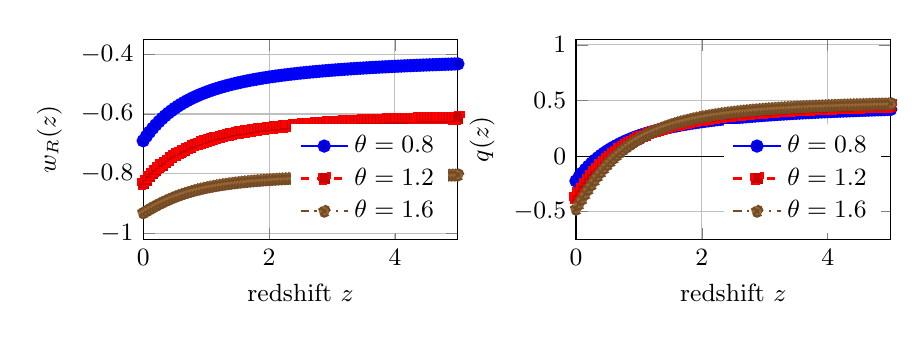
\begin{tikzpicture}
\begin{groupplot}[
  group style={group size=2 by 1, horizontal sep=1.5cm},
  width=0.46\textwidth,
  height=0.34\textwidth,
  grid=both,
  xmin=0, xmax=5,
  legend style={font=\small, draw=none},
  tick label style={font=\small},
  label style={font=\small}
]
\nextgroupplot[
  xlabel={redshift \(z\)},
  ylabel={\(w_R(z)\)},
  ymin=-1.02, ymax=-0.35,
  legend pos=south east
]
\addplot+[thick] coordinates {
(0.0000,-0.68955994)
(0.0500,-0.67463575)
(0.1000,-0.66081693)
(0.1500,-0.64802549)
(0.2000,-0.63618249)
(0.2500,-0.62521096)
(0.3000,-0.61503771)
(0.3500,-0.60559426)
(0.4000,-0.59681732)
(0.4500,-0.58864885)
(0.5000,-0.58103592)
(0.5500,-0.57393048)
(0.6000,-0.56728897)
(0.6500,-0.56107201)
(0.7000,-0.55524401)
(0.7500,-0.54977280)
(0.8000,-0.54462932)
(0.8500,-0.53978731)
(0.9000,-0.53522298)
(0.9500,-0.53091482)
(1.0000,-0.52684330)
(1.0500,-0.52299072)
(1.1000,-0.51934097)
(1.1500,-0.51587940)
(1.2000,-0.51259266)
(1.2500,-0.50946857)
(1.3000,-0.50649600)
(1.3500,-0.50366476)
(1.4000,-0.50096551)
(1.4500,-0.49838969)
(1.5000,-0.49592942)
(1.5500,-0.49357747)
(1.6000,-0.49132717)
(1.6500,-0.48917234)
(1.7000,-0.48710732)
(1.7500,-0.48512684)
(1.8000,-0.48322603)
(1.8500,-0.48140037)
(1.9000,-0.47964567)
(1.9500,-0.47795805)
(2.0000,-0.47633387)
(2.0500,-0.47476976)
(2.1000,-0.47326258)
(2.1500,-0.47180938)
(2.2000,-0.47040743)
(2.2500,-0.46905416)
(2.3000,-0.46774716)
(2.3500,-0.46648420)
(2.4000,-0.46526315)
(2.4500,-0.46408203)
(2.5000,-0.46293899)
(2.5500,-0.46183228)
(2.6000,-0.46076024)
(2.6500,-0.45972133)
(2.7000,-0.45871408)
(2.7500,-0.45773712)
(2.8000,-0.45678914)
(2.8500,-0.45586892)
(2.9000,-0.45497528)
(2.9500,-0.45410714)
(3.0000,-0.45326344)
(3.0500,-0.45244320)
(3.1000,-0.45164549)
(3.1500,-0.45086941)
(3.2000,-0.45011413)
(3.2500,-0.44937885)
(3.3000,-0.44866280)
(3.3500,-0.44796526)
(3.4000,-0.44728555)
(3.4500,-0.44662300)
(3.5000,-0.44597699)
(3.5500,-0.44534694)
(3.6000,-0.44473227)
(3.6500,-0.44413244)
(3.7000,-0.44354694)
(3.7500,-0.44297526)
(3.8000,-0.44241695)
(3.8500,-0.44187155)
(3.9000,-0.44133863)
(3.9500,-0.44081777)
(4.0000,-0.44030859)
(4.0500,-0.43981070)
(4.1000,-0.43932375)
(4.1500,-0.43884738)
(4.2000,-0.43838126)
(4.2500,-0.43792508)
(4.3000,-0.43747853)
(4.3500,-0.43704131)
(4.4000,-0.43661314)
(4.4500,-0.43619375)
(4.5000,-0.43578288)
(4.5500,-0.43538027)
(4.6000,-0.43498570)
(4.6500,-0.43459892)
(4.7000,-0.43421971)
(4.7500,-0.43384786)
(4.8000,-0.43348316)
(4.8500,-0.43312541)
(4.9000,-0.43277442)
(4.9500,-0.43243000)
(5.0000,-0.43209197)
};
\addlegendentry{\(\theta=0.8\)}
\addplot+[thick,dashed] coordinates {
(0.0000,-0.83327500)
(0.0500,-0.82139201)
(0.1000,-0.81007780)
(0.1500,-0.79935155)
(0.2000,-0.78921706)
(0.2500,-0.77966658)
(0.3000,-0.77068398)
(0.3500,-0.76224740)
(0.4000,-0.75433124)
(0.4500,-0.74690780)
(0.5000,-0.73994844)
(0.5500,-0.73342444)
(0.6000,-0.72730759)
(0.6500,-0.72157066)
(0.7000,-0.71618766)
(0.7500,-0.71113396)
(0.8000,-0.70638642)
(0.8500,-0.70192339)
(0.9000,-0.69772469)
(0.9500,-0.69377159)
(1.0000,-0.69004672)
(1.0500,-0.68653402)
(1.1000,-0.68321862)
(1.1500,-0.68008682)
(1.2000,-0.67712596)
(1.2500,-0.67432437)
(1.3000,-0.67167127)
(1.3500,-0.66915672)
(1.4000,-0.66677155)
(1.4500,-0.66450728)
(1.5000,-0.66235609)
(1.5500,-0.66031075)
(1.6000,-0.65836457)
(1.6500,-0.65651135)
(1.7000,-0.65474538)
(1.7500,-0.65306133)
(1.8000,-0.65145427)
(1.8500,-0.64991965)
(1.9000,-0.64845321)
(1.9500,-0.64705100)
(2.0000,-0.64570936)
(2.0500,-0.64442486)
(2.1000,-0.64319432)
(2.1500,-0.64201477)
(2.2000,-0.64088344)
(2.2500,-0.63979773)
(2.3000,-0.63875524)
(2.3500,-0.63775368)
(2.4000,-0.63679096)
(2.4500,-0.63586507)
(2.5000,-0.63497416)
(2.5500,-0.63411648)
(2.6000,-0.63329040)
(2.6500,-0.63249438)
(2.7000,-0.63172695)
(2.7500,-0.63098678)
(2.8000,-0.63027256)
(2.8500,-0.62958309)
(2.9000,-0.62891724)
(2.9500,-0.62827392)
(3.0000,-0.62765212)
(3.0500,-0.62705090)
(3.1000,-0.62646933)
(3.1500,-0.62590656)
(3.2000,-0.62536179)
(3.2500,-0.62483424)
(3.3000,-0.62432319)
(3.3500,-0.62382795)
(3.4000,-0.62334787)
(3.4500,-0.62288233)
(3.5000,-0.62243073)
(3.5500,-0.62199252)
(3.6000,-0.62156717)
(3.6500,-0.62115418)
(3.7000,-0.62075305)
(3.7500,-0.62036334)
(3.8000,-0.61998461)
(3.8500,-0.61961645)
(3.9000,-0.61925845)
(3.9500,-0.61891025)
(4.0000,-0.61857148)
(4.0500,-0.61824180)
(4.1000,-0.61792088)
(4.1500,-0.61760841)
(4.2000,-0.61730409)
(4.2500,-0.61700763)
(4.3000,-0.61671877)
(4.3500,-0.61643723)
(4.4000,-0.61616277)
(4.4500,-0.61589515)
(4.5000,-0.61563413)
(4.5500,-0.61537951)
(4.6000,-0.61513106)
(4.6500,-0.61488859)
(4.7000,-0.61465190)
(4.7500,-0.61442080)
(4.8000,-0.61419512)
(4.8500,-0.61397469)
(4.9000,-0.61375934)
(4.9500,-0.61354890)
(5.0000,-0.61334324)
};
\addlegendentry{\(\theta=1.2\)}
\addplot+[thick,dashdotted] coordinates {
(0.0000,-0.93020611)
(0.0500,-0.92391970)
(0.1000,-0.91777406)
(0.1500,-0.91180817)
(0.2000,-0.90605177)
(0.2500,-0.90052619)
(0.3000,-0.89524549)
(0.3500,-0.89021746)
(0.4000,-0.88544480)
(0.4500,-0.88092612)
(0.5000,-0.87665683)
(0.5500,-0.87262994)
(0.6000,-0.86883672)
(0.6500,-0.86526727)
(0.7000,-0.86191093)
(0.7500,-0.85875666)
(0.8000,-0.85579330)
(0.8500,-0.85300976)
(0.9000,-0.85039522)
(0.9500,-0.84793919)
(1.0000,-0.84563162)
(1.0500,-0.84346294)
(1.1000,-0.84142406)
(1.1500,-0.83950644)
(1.2000,-0.83770201)
(1.2500,-0.83600325)
(1.3000,-0.83440311)
(1.3500,-0.83289500)
(1.4000,-0.83147280)
(1.4500,-0.83013081)
(1.5000,-0.82886371)
(1.5500,-0.82766657)
(1.6000,-0.82653481)
(1.6500,-0.82546419)
(1.7000,-0.82445074)
(1.7500,-0.82349081)
(1.8000,-0.82258098)
(1.8500,-0.82171809)
(1.9000,-0.82089921)
(1.9500,-0.82012161)
(2.0000,-0.81938274)
(2.0500,-0.81868024)
(2.1000,-0.81801193)
(2.1500,-0.81737576)
(2.2000,-0.81676983)
(2.2500,-0.81619236)
(2.3000,-0.81564171)
(2.3500,-0.81511633)
(2.4000,-0.81461478)
(2.4500,-0.81413573)
(2.5000,-0.81367792)
(2.5500,-0.81324017)
(2.6000,-0.81282139)
(2.6500,-0.81242056)
(2.7000,-0.81203671)
(2.7500,-0.81166895)
(2.8000,-0.81131642)
(2.8500,-0.81097834)
(2.9000,-0.81065397)
(2.9500,-0.81034260)
(3.0000,-0.81004358)
(3.0500,-0.80975630)
(3.1000,-0.80948018)
(3.1500,-0.80921466)
(3.2000,-0.80895923)
(3.2500,-0.80871342)
(3.3000,-0.80847675)
(3.3500,-0.80824881)
(3.4000,-0.80802919)
(3.4500,-0.80781749)
(3.5000,-0.80761336)
(3.5500,-0.80741646)
(3.6000,-0.80722645)
(3.6500,-0.80704304)
(3.7000,-0.80686593)
(3.7500,-0.80669485)
(3.8000,-0.80652953)
(3.8500,-0.80636973)
(3.9000,-0.80621522)
(3.9500,-0.80606576)
(4.0000,-0.80592116)
(4.0500,-0.80578120)
(4.1000,-0.80564570)
(4.1500,-0.80551448)
(4.2000,-0.80538736)
(4.2500,-0.80526418)
(4.3000,-0.80514479)
(4.3500,-0.80502903)
(4.4000,-0.80491676)
(4.4500,-0.80480785)
(4.5000,-0.80470217)
(4.5500,-0.80459959)
(4.6000,-0.80450000)
(4.6500,-0.80440329)
(4.7000,-0.80430935)
(4.7500,-0.80421808)
(4.8000,-0.80412937)
(4.8500,-0.80404315)
(4.9000,-0.80395931)
(4.9500,-0.80387777)
(5.0000,-0.80379846)
};
\addlegendentry{\(\theta=1.6\)}

\nextgroupplot[
  xlabel={redshift \(z\)},
  ylabel={\(q(z)\)},
  ymin=-0.75, ymax=1.05,
  legend pos=south east
]
\addplot+[thick] coordinates {
(0.0000,-0.22389984)
(0.0500,-0.18658938)
(0.1000,-0.15204232)
(0.1500,-0.12006372)
(0.2000,-0.09045622)
(0.2500,-0.06302740)
(0.3000,-0.03759426)
(0.3500,-0.01398564)
(0.4000,0.00795671)
(0.4500,0.02837788)
(0.5000,0.04741019)
(0.5500,0.06517380)
(0.6000,0.08177758)
(0.6500,0.09731998)
(0.7000,0.11188999)
(0.7500,0.12556801)
(0.8000,0.13842670)
(0.8500,0.15053174)
(0.9000,0.16194255)
(0.9500,0.17271295)
(1.0000,0.18289174)
(1.0500,0.19252320)
(1.1000,0.20164758)
(1.1500,0.21030150)
(1.2000,0.21851835)
(1.2500,0.22632857)
(1.3000,0.23376000)
(1.3500,0.24083810)
(1.4000,0.24758623)
(1.4500,0.25402578)
(1.5000,0.26017644)
(1.5500,0.26605631)
(1.6000,0.27168208)
(1.6500,0.27706914)
(1.7000,0.28223170)
(1.7500,0.28718290)
(1.8000,0.29193494)
(1.8500,0.29649908)
(1.9000,0.30088581)
(1.9500,0.30510488)
(2.0000,0.30916533)
(2.0500,0.31307560)
(2.1000,0.31684356)
(2.1500,0.32047655)
(2.2000,0.32398142)
(2.2500,0.32736460)
(2.3000,0.33063209)
(2.3500,0.33378951)
(2.4000,0.33684213)
(2.4500,0.33979492)
(2.5000,0.34265252)
(2.5500,0.34541931)
(2.6000,0.34809940)
(2.6500,0.35069668)
(2.7000,0.35321479)
(2.7500,0.35565720)
(2.8000,0.35802714)
(2.8500,0.36032770)
(2.9000,0.36256179)
(2.9500,0.36473216)
(3.0000,0.36684140)
(3.0500,0.36889200)
(3.1000,0.37088628)
(3.1500,0.37282647)
(3.2000,0.37471466)
(3.2500,0.37655288)
(3.3000,0.37834300)
(3.3500,0.38008685)
(3.4000,0.38178614)
(3.4500,0.38344250)
(3.5000,0.38505751)
(3.5500,0.38663265)
(3.6000,0.38816932)
(3.6500,0.38966890)
(3.7000,0.39113266)
(3.7500,0.39256184)
(3.8000,0.39395762)
(3.8500,0.39532113)
(3.9000,0.39665343)
(3.9500,0.39795557)
(4.0000,0.39922853)
(4.0500,0.40047325)
(4.1000,0.40169063)
(4.1500,0.40288155)
(4.2000,0.40404684)
(4.2500,0.40518730)
(4.3000,0.40630368)
(4.3500,0.40739674)
(4.4000,0.40846716)
(4.4500,0.40951563)
(4.5000,0.41054281)
(4.5500,0.41154931)
(4.6000,0.41253575)
(4.6500,0.41350270)
(4.7000,0.41445072)
(4.7500,0.41538035)
(4.8000,0.41629210)
(4.8500,0.41718648)
(4.9000,0.41806396)
(4.9500,0.41892501)
(5.0000,0.41977008)
};
\addlegendentry{\(\theta=0.8\)}
\addplot+[thick,dashed] coordinates {
(0.0000,-0.37478126)
(0.0500,-0.33022004)
(0.1000,-0.28779176)
(0.1500,-0.24756832)
(0.2000,-0.20956399)
(0.2500,-0.17374968)
(0.3000,-0.14006494)
(0.3500,-0.10842774)
(0.4000,-0.07874214)
(0.4500,-0.05090426)
(0.5000,-0.02480667)
(0.5500,-0.00034163)
(0.6000,0.02259655)
(0.6500,0.04411001)
(0.7000,0.06429627)
(0.7500,0.08324764)
(0.8000,0.10105092)
(0.8500,0.11778729)
(0.9000,0.13353240)
(0.9500,0.14835653)
(1.0000,0.16232479)
(1.0500,0.17549744)
(1.1000,0.18793019)
(1.1500,0.19967443)
(1.2000,0.21077765)
(1.2500,0.22128362)
(1.3000,0.23123274)
(1.3500,0.24066230)
(1.4000,0.24960669)
(1.4500,0.25809770)
(1.5000,0.26616465)
(1.5500,0.27383468)
(1.6000,0.28113287)
(1.6500,0.28808242)
(1.7000,0.29470484)
(1.7500,0.30102003)
(1.8000,0.30704647)
(1.8500,0.31280131)
(1.9000,0.31830046)
(1.9500,0.32355874)
(2.0000,0.32858990)
(2.0500,0.33340677)
(2.1000,0.33802129)
(2.1500,0.34244460)
(2.2000,0.34668710)
(2.2500,0.35075850)
(2.3000,0.35466786)
(2.3500,0.35842369)
(2.4000,0.36203392)
(2.4500,0.36550600)
(2.5000,0.36884690)
(2.5500,0.37206318)
(2.6000,0.37516099)
(2.6500,0.37814609)
(2.7000,0.38102392)
(2.7500,0.38379959)
(2.8000,0.38647791)
(2.8500,0.38906341)
(2.9000,0.39156037)
(2.9500,0.39397281)
(3.0000,0.39630453)
(3.0500,0.39855914)
(3.1000,0.40074002)
(3.1500,0.40285040)
(3.2000,0.40489329)
(3.2500,0.40687160)
(3.3000,0.40878803)
(3.3500,0.41064518)
(3.4000,0.41244548)
(3.4500,0.41419128)
(3.5000,0.41588477)
(3.5500,0.41752805)
(3.6000,0.41912311)
(3.6500,0.42067184)
(3.7000,0.42217606)
(3.7500,0.42363747)
(3.8000,0.42505770)
(3.8500,0.42643832)
(3.9000,0.42778080)
(3.9500,0.42908656)
(4.0000,0.43035694)
(4.0500,0.43159325)
(4.1000,0.43279669)
(4.1500,0.43396845)
(4.2000,0.43510966)
(4.2500,0.43622137)
(4.3000,0.43730462)
(4.3500,0.43836039)
(4.4000,0.43938961)
(4.4500,0.44039320)
(4.5000,0.44137200)
(4.5500,0.44232684)
(4.6000,0.44325852)
(4.6500,0.44416779)
(4.7000,0.44505538)
(4.7500,0.44592199)
(4.8000,0.44676828)
(4.8500,0.44759491)
(4.9000,0.44840249)
(4.9500,0.44919161)
(5.0000,0.44996284)
};
\addlegendentry{\(\theta=1.2\)}
\addplot+[thick,dashdotted] coordinates {
(0.0000,-0.47654584)
(0.0500,-0.42939776)
(0.1000,-0.38330546)
(0.1500,-0.33856129)
(0.2000,-0.29538824)
(0.2500,-0.25394646)
(0.3000,-0.21434115)
(0.3500,-0.17663092)
(0.4000,-0.14083601)
(0.4500,-0.10694591)
(0.5000,-0.07492623)
(0.5500,-0.04472454)
(0.6000,-0.01627541)
(0.6500,0.01049547)
(0.7000,0.03566801)
(0.7500,0.05932503)
(0.8000,0.08155028)
(0.8500,0.10242681)
(0.9000,0.12203586)
(0.9500,0.14045607)
(1.0000,0.15776281)
(1.0500,0.17402795)
(1.1000,0.18931952)
(1.1500,0.20370173)
(1.2000,0.21723491)
(1.2500,0.22997561)
(1.3000,0.24197669)
(1.3500,0.25328749)
(1.4000,0.26395398)
(1.4500,0.27401895)
(1.5000,0.28352221)
(1.5500,0.29250074)
(1.6000,0.30098889)
(1.6500,0.30901858)
(1.7000,0.31661942)
(1.7500,0.32381893)
(1.8000,0.33064265)
(1.8500,0.33711429)
(1.9000,0.34325591)
(1.9500,0.34908796)
(2.0000,0.35462949)
(2.0500,0.35989818)
(2.1000,0.36491050)
(2.1500,0.36968178)
(2.2000,0.37422627)
(2.2500,0.37855727)
(2.3000,0.38268718)
(2.3500,0.38662754)
(2.4000,0.39038913)
(2.4500,0.39398203)
(2.5000,0.39741563)
(2.5500,0.40069873)
(2.6000,0.40383956)
(2.6500,0.40684580)
(2.7000,0.40972467)
(2.7500,0.41248291)
(2.8000,0.41512685)
(2.8500,0.41766244)
(2.9000,0.42009524)
(2.9500,0.42243049)
(3.0000,0.42467311)
(3.0500,0.42682773)
(3.1000,0.42889868)
(3.1500,0.43089007)
(3.2000,0.43280576)
(3.2500,0.43464938)
(3.3000,0.43642435)
(3.3500,0.43813391)
(3.4000,0.43978111)
(3.4500,0.44136883)
(3.5000,0.44289980)
(3.5500,0.44437658)
(3.6000,0.44580161)
(3.6500,0.44717720)
(3.7000,0.44850552)
(3.7500,0.44978864)
(3.8000,0.45102851)
(3.8500,0.45222700)
(3.9000,0.45338587)
(3.9500,0.45450677)
(4.0000,0.45559131)
(4.0500,0.45664098)
(4.1000,0.45765722)
(4.1500,0.45864139)
(4.2000,0.45959478)
(4.2500,0.46051862)
(4.3000,0.46141409)
(4.3500,0.46228230)
(4.4000,0.46312431)
(4.4500,0.46394114)
(4.5000,0.46473376)
(4.5500,0.46550309)
(4.6000,0.46624999)
(4.6500,0.46697533)
(4.7000,0.46767989)
(4.7500,0.46836444)
(4.8000,0.46902971)
(4.8500,0.46967640)
(4.9000,0.47030519)
(4.9500,0.47091670)
(5.0000,0.47151156)
};
\addlegendentry{\(\theta=1.6\)}
\addplot[black,thin,mark=none] coordinates {(0,0) (5,0)};
\end{groupplot}
\end{tikzpicture}
\caption{Cosmological dynamics evaluated from the homogeneous RFG equations and rendered from numerical coordinates embedded in this \LaTeX{} source. The left panel shows \(w_R(z)\), and the right panel shows \(q(z)\), for three representative values of \(\theta\). The acceleration transition \(q=0\) coincides with \(\Omega_R(z_{\rm acc})=1/(1+\theta)\). Parameters: \(\Omega_{m0}=0.3\), \(\Omega_{r0}=9\times10^{-5}\), and \(\Omega_{R0}=1-\Omega_{m0}-\Omega_{r0}\).}
\label{fig:cosmo}
\end{figure}
\FloatBarrier

\subsection{Early- and late-time asymptotics}

At early times \(E\to\infty\), so \(\Omega_R=\Omega_{R0}E^{-\theta}\to0\). The standard radiation- and matter-dominated limits are therefore recovered. The future attractor is de~Sitter with
\[
E_\infty=\Omega_{R0}^{1/\theta},\qquad H_\infty=H_0\Omega_{R0}^{1/\theta}.
\]

\subsection{Tensor sector and standard-siren ratio}

The quadratic action for transverse-traceless modes is
\begin{equation}
S_T^{(2)}=\frac{\mpl^2}{8}\int\dd t\,\dd^3x\,a^3Q_T\Bigl[\dot h_{ij}\dot h_{ij}-\frac{\partial_k h_{ij}\partial_k h_{ij}}{a^2}\Bigr],
\end{equation}
with
\[
\Boxed{Q_T(a)=1-\frac{\Omega_R(a)}{1+\theta},\qquad c_T^2=1.}
\]
The no-ghost condition \(Q_T>0\) holds throughout the homogeneous branch for \(\theta>0\). The standard-siren amplitude relation follows at once:
\begin{equation}
\Boxed{\frac{d_L^{\rm GW}(z)}{d_L^{\rm EM}(z)}=\sqrt{\frac{Q_T(0)}{Q_T(z)}}.}
\label{eq:siren}
\end{equation}

Equation~\eqref{eq:siren} is the WKB/subhorizon tensor-amplitude result under the following assumptions: matter is minimally coupled to the metric \(g_{\mu\nu}\), photons and gravitational waves share the same background redshift relation, there is no tensor mixing with an additional propagating spin--2 field, and the observed Planck normalization is fixed at \(z=0\). Under these assumptions \(Q_T\) modifies only the tensor friction term, not the null cone, which is why \(c_T=1\) and the distance ratio in Eq.~\eqref{eq:siren} can differ from unity simultaneously.

\begin{remark}[Order-of-magnitude estimate]
For a representative late-time branch with \(\Omega_{R0}\approx0.7\) and \(\theta\approx1.6\) one obtains \(Q_T(0)\approx0.73\). At high redshift \(\Omega_R\to0\), so \(Q_T\to1\) and the ratio approaches \(\sqrt{Q_T(0)}\approx0.85\). At redshift \(z=1\) the same branch yields a ratio of order \(0.9\). The near-luminal propagation constraint from GW170817 is automatically respected because \(c_T=1\)~\cite{GW170817}. The amplitude-distance modification is instead a standard-siren observable of the type discussed in forecast studies~\cite{Belgacem}. The corresponding curve is shown in Fig.~\ref{fig:siren}. A dedicated likelihood comparison is left for future work.
\end{remark}

\begin{figure}[H]
\centering
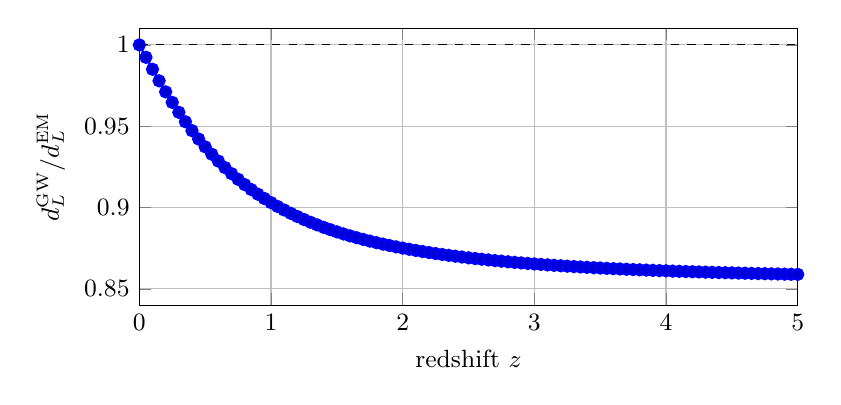
\begin{tikzpicture}
\begin{axis}[
  width=0.82\textwidth,
  height=0.42\textwidth,
  xlabel={redshift \(z\)},
  ylabel={\(d_L^{\rm GW}/d_L^{\rm EM}\)},
  xmin=0, xmax=5,
  ymin=0.84, ymax=1.01,
  grid=both,
  tick label style={font=\small},
  label style={font=\small}
]
\addplot+[thick] coordinates {
(0.0000,1.00000000)
(0.0500,0.99238993)
(0.1000,0.98501840)
(0.1500,0.97792548)
(0.2000,0.97113918)
(0.2500,0.96467707)
(0.3000,0.95854805)
(0.3500,0.95275393)
(0.4000,0.94729098)
(0.4500,0.94215130)
(0.5000,0.93732390)
(0.5500,0.93279569)
(0.6000,0.92855222)
(0.6500,0.92457829)
(0.7000,0.92085841)
(0.7500,0.91737715)
(0.8000,0.91411937)
(0.8500,0.91107048)
(0.9000,0.90821647)
(0.9500,0.90554405)
(1.0000,0.90304066)
(1.0500,0.90069451)
(1.1000,0.89849456)
(1.1500,0.89643050)
(1.2000,0.89449276)
(1.2500,0.89267243)
(1.3000,0.89096124)
(1.3500,0.88935156)
(1.4000,0.88783631)
(1.4500,0.88640892)
(1.5000,0.88506335)
(1.5500,0.88379399)
(1.6000,0.88259568)
(1.6500,0.88146362)
(1.7000,0.88039340)
(1.7500,0.87938091)
(1.8000,0.87842238)
(1.8500,0.87751431)
(1.9000,0.87665344)
(1.9500,0.87583678)
(2.0000,0.87506154)
(2.0500,0.87432514)
(2.1000,0.87362518)
(2.1500,0.87295943)
(2.2000,0.87232583)
(2.2500,0.87172246)
(2.3000,0.87114753)
(2.3500,0.87059937)
(2.4000,0.87007644)
(2.4500,0.86957729)
(2.5000,0.86910057)
(2.5500,0.86864503)
(2.6000,0.86820949)
(2.6500,0.86779285)
(2.7000,0.86739408)
(2.7500,0.86701224)
(2.8000,0.86664641)
(2.8500,0.86629575)
(2.9000,0.86595948)
(2.9500,0.86563685)
(3.0000,0.86532717)
(3.0500,0.86502978)
(3.1000,0.86474407)
(3.1500,0.86446946)
(3.2000,0.86420540)
(3.2500,0.86395140)
(3.3000,0.86370695)
(3.3500,0.86347162)
(3.4000,0.86324496)
(3.4500,0.86302658)
(3.5000,0.86281609)
(3.5500,0.86261314)
(3.6000,0.86241737)
(3.6500,0.86222848)
(3.7000,0.86204614)
(3.7500,0.86187009)
(3.8000,0.86170003)
(3.8500,0.86153571)
(3.9000,0.86137689)
(3.9500,0.86122333)
(4.0000,0.86107482)
(4.0500,0.86093113)
(4.1000,0.86079207)
(4.1500,0.86065746)
(4.2000,0.86052711)
(4.2500,0.86040084)
(4.3000,0.86027850)
(4.3500,0.86015994)
(4.4000,0.86004500)
(4.4500,0.85993354)
(4.5000,0.85982542)
(4.5500,0.85972053)
(4.6000,0.85961874)
(4.6500,0.85951992)
(4.7000,0.85942398)
(4.7500,0.85933080)
(4.8000,0.85924028)
(4.8500,0.85915233)
(4.9000,0.85906685)
(4.9500,0.85898375)
(5.0000,0.85890295)
};
\addplot[black,thin,dashed,mark=none] coordinates {(0,1) (5,1)};
\end{axis}
\end{tikzpicture}
\caption{Standard-siren prediction evaluated from Eq.~\eqref{eq:siren} on the homogeneous RFG background and rendered from numerical coordinates embedded in this \LaTeX{} source, for \(\Omega_{R0}=0.70\) and \(\theta=1.6\). The ratio equals unity at \(z=0\), is approximately \(0.903\) at \(z=1\), and approaches \(\sqrt{Q_T(0)}\approx0.855\) at high redshift. No illustrative observational point is added, because a statistically meaningful comparison requires an explicit likelihood analysis.}
\label{fig:siren}
\end{figure}
\FloatBarrier


%====================================================
\section{RFG-R: regular multiscale effective completion}
\label{sec:rfg-r}

The original branch in Eqs.~\eqref{eq:Q}--\eqref{eq:V} is singular at
\(X=0\) when \(\theta>0\). It therefore cannot by itself support a standard
asymptotically flat weak-field expansion. This section defines a different,
low-energy effective theory, called RFG-R. It is constructed to retain the
cosmological branch to a controlled accuracy, to be regular at \(X=0\), and
to state the local matching rule rather than silently extrapolating a
homogeneous action into Solar-System geometry. RFG-R is a model definition;
it is not claimed to follow uniquely from the original RFG action.

\subsection{Regular cosmological action and exact reconstruction}

Let \(p\) be an even integer satisfying \(p>\theta\), let
\(\epsilon>0\), and define
\begin{equation}
 \nu:=1+\frac{\theta}{p},\qquad
 A:=\frac{\Omega_{R0}}{1+\theta}.
\end{equation}
The regular response and tensor normalization are
\begin{align}
 \mathcal R_\epsilon(X)&:=
 \Omega_{R0}\frac{X^{p+2}}{\left(X^p+\epsilon^p\right)^\nu},
 \label{eq:RFGR-response}\\
 Q_\epsilon(X)&:=1-A\frac{X^p}{\left(X^p+\epsilon^p\right)^\nu}.
 \label{eq:RFGR-Q}
\end{align}
The cosmological RFG-R action is
\begin{equation}
 S_{\rm cos}=\frac{\mpl^2}{2}\int\dd^4x\sqrt{-g}\,
 \left[Q_\epsilon(X)\left({}^{(3)}R+K_{\mu\nu}K^{\mu\nu}-K^2\right)
 +2H_0^2V_\epsilon(X)\right]+S_m[g,\Psi].
 \label{eq:RFGR-cosmological-action}
\end{equation}
Matter is minimally and universally coupled to the Jordan metric \(g_{\mu\nu}\).
Define
\begin{equation}
 F_\epsilon(X):=X^2-\mathcal R_\epsilon(X)-X^2Q_\epsilon(X)
 -X^3Q_{\epsilon,X}(X).
 \label{eq:RFGR-F}
\end{equation}
The FLRW lapse equation has the target form
\begin{equation}
 \boxed{E^2=\Omega_{m0}a^{-3}+\Omega_{r0}a^{-4}+\mathcal R_\epsilon(E).}
 \label{eq:RFGR-background}
\end{equation}
Comparison with Eq.~\eqref{eq:FLRW-constraint-general} fixes the potential,
up to the usual ADM boundary representative \(CX\), through
\begin{align}
 V_\epsilon-XV_{\epsilon,X}&=3F_\epsilon(X),\\
 \boxed{V_\epsilon(X)=-3X\int_0^X\frac{F_\epsilon(s)}{s^2}\,\dd s.}
 \label{eq:RFGR-potential}
\end{align}
The integrand is finite at the origin. Thus Eq.~\eqref{eq:RFGR-potential} is
an action-level reconstruction, not a background-only prescription.

For \(X\gg\epsilon\),
\begin{align}
 \mathcal R_\epsilon(X)&=\Omega_{R0}X^{2-\theta}
 \left[1-\left(1+\frac{\theta}{p}\right)
 \left(\frac{\epsilon}{X}\right)^p+O\left((\epsilon/X)^{2p}\right)\right],\\
 Q_\epsilon(X)&=1-AX^{-\theta}
 \left[1-\left(1+\frac{\theta}{p}\right)
 \left(\frac{\epsilon}{X}\right)^p+O\left((\epsilon/X)^{2p}\right)\right].
 \label{eq:RFGR-recovery}
\end{align}
The reference choice \(p=4\), \(\epsilon=10^{-8}\), and \(\theta=1.6\)
therefore changes the original branch by at most \(2.5\times10^{-32}\) for
\(X\geq0.8\), analytically. At small \(X\), \(Q_\epsilon(0)=1\) and
\(V_\epsilon=O(X^{p+2})\), so the Einstein--Hilbert ADM kinetic operator is
recovered at \(K=0\). Figure~\ref{fig:rfgr-regularization} displays the
numerical recovery and regularization check. The resulting radiation, matter,
and relational fractions on the same regularized expanding branch are shown
in Fig.~\ref{fig:rfgr-background-fractions}.

\begin{figure}[H]
\centering
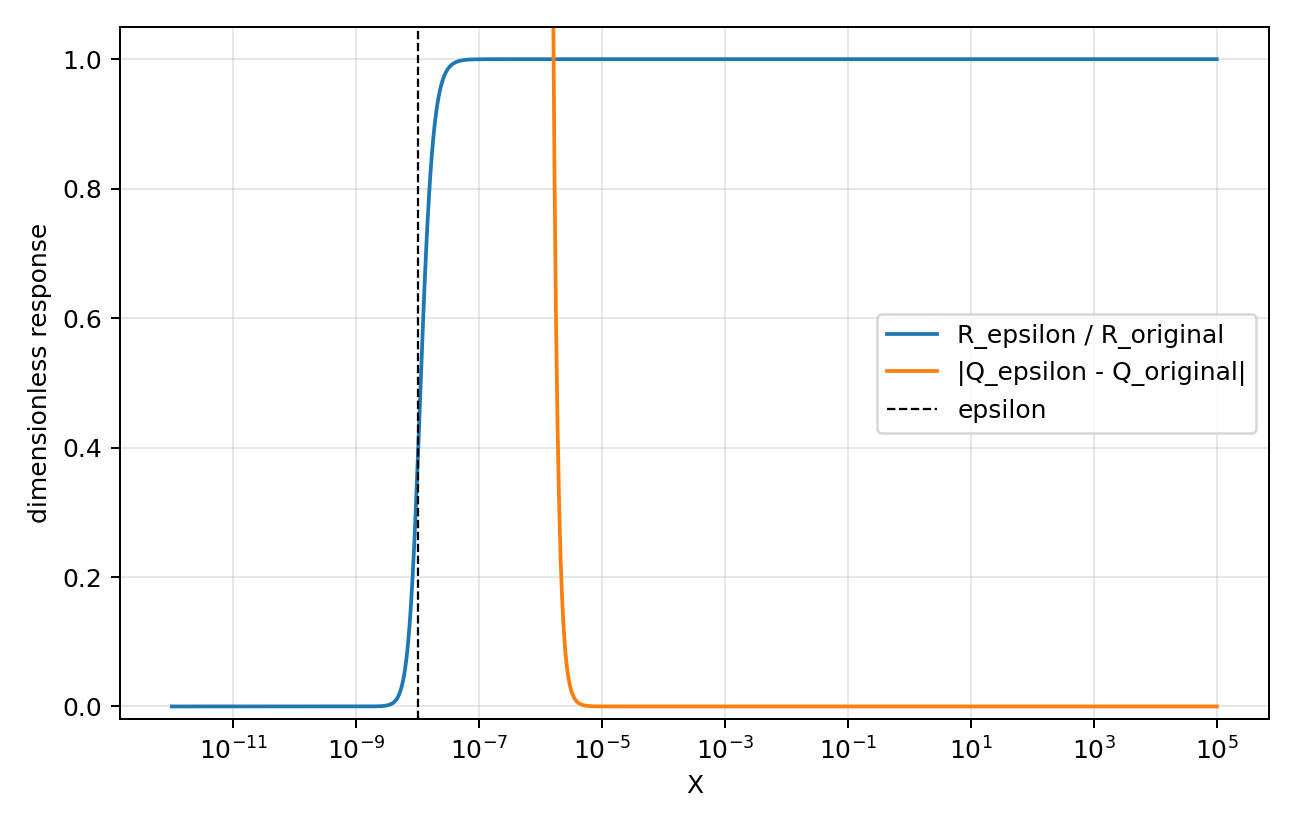
\includegraphics[width=0.82\textwidth]{download.png}
\caption{RFG-R regularization check. The response ratio
\(\mathcal R_\epsilon/\mathcal R_{\rm original}\) and the tensor-normalization
difference \(\lvert Q_\epsilon-Q_{\rm original}\rvert\) are evaluated with
\(p=4\), \(\epsilon=10^{-8}\), and \(\theta=1.6\). Above the regulated
\(X\simeq\epsilon\) domain, RFG-R recovers the original cosmological branch;
the analytic high-\(X\) error is given in Eq.~\eqref{eq:RFGR-recovery}.
This is an action-level numerical validation, not an observational fit.
The generating script is \RFGRepoNamed{scripts/generate\_outputs.py}{output generator}.}
\label{fig:rfgr-regularization}
\end{figure}

\begin{figure}[H]
\centering
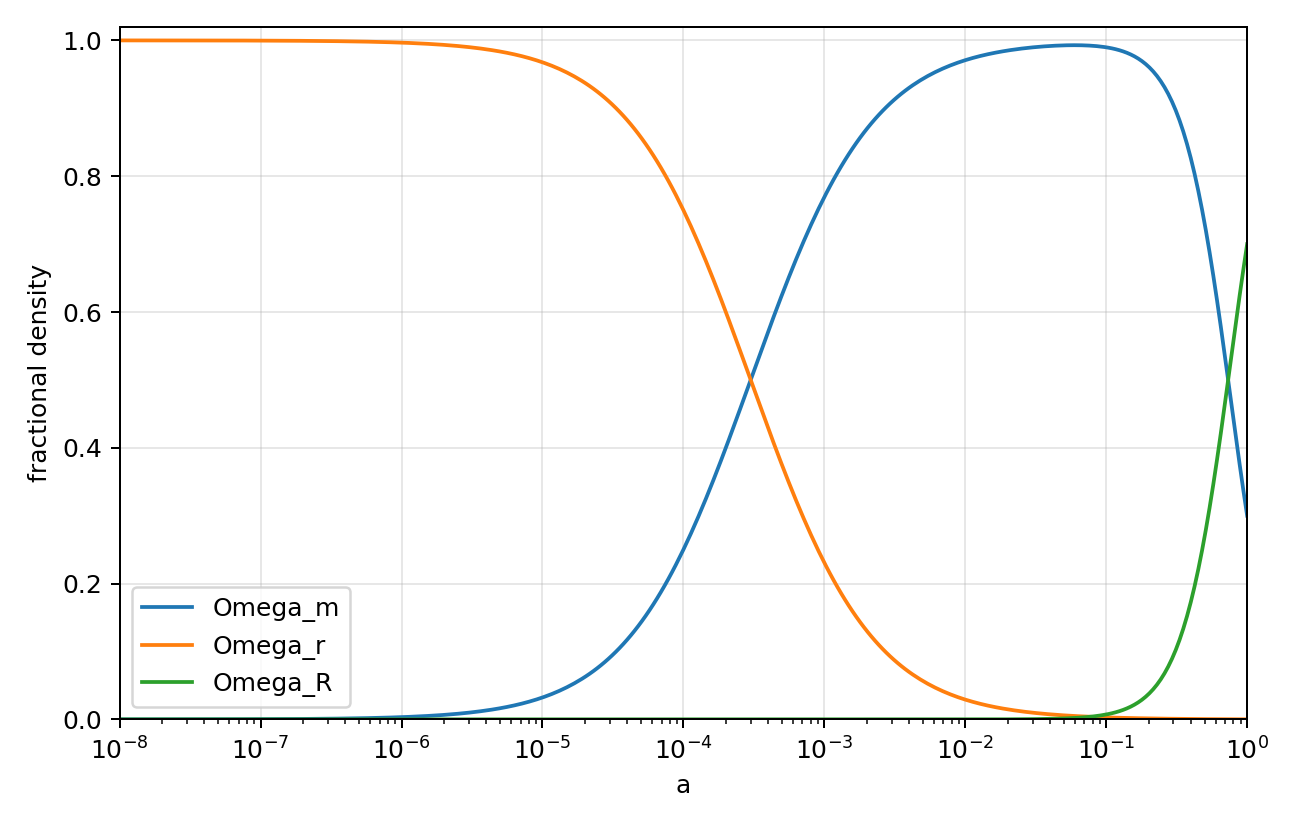
\includegraphics[width=0.82\textwidth]{download-1.png}
\caption{Fractional densities on the regularized RFG-R expanding branch of
Eq.~\eqref{eq:RFGR-background}, with
\(\Omega_{m0}=0.30\), \(\Omega_{r0}=9\times10^{-5}\),
\(\Omega_{R0}=0.69991\), \(\theta=1.6\), \(p=4\), and
\(\epsilon=10^{-8}\). The curves show radiation, matter, and relational
components computed from the action-reconstructed background equation. They
are not a compressed CMB constraint. The generating script is
\RFGRepoNamed{scripts/generate\_outputs.py}{output generator}.}
\label{fig:rfgr-background-fractions}
\end{figure}
\FloatBarrier

\subsection{Local GR matching and PPN statement}

The cosmological action is supplemented by an explicit multiscale matching
rule. Let
\begin{equation}
 W:=\frac{\sqrt{\lvert C_{\alpha\beta\gamma\delta}
 C^{\alpha\beta\gamma\delta}\rvert}}{(H_0/c)^2}.
 \label{eq:RFGR-Weyl}
\end{equation}
Choose a \(C^\infty\) switch \(s(W)\) with \(s=1\) for \(W\leq10^8\)
and \(s=0\) for \(W\geq10^9\); its explicit bump-function construction is
given in \RFGRepoNamed{docs/completion\_derivation.md}{completion derivation}. The complete
low-energy EFT is
\begin{equation}
 S_{\rm eff}=S_{\rm GR}+\int\dd^4x\,s(W)
 \left(\mathcal L_{\rm cos}-\mathcal L_{\rm GR}\right).
 \label{eq:RFGR-matching}
\end{equation}
Here \(\mathcal L\) denotes the corresponding covariant action density,
including \(\sqrt{-g}\). Flat FLRW has \(W=0\), hence uses the cosmological
action. In every open region with \(W\geq10^9\), both \(s\) and all its
derivatives vanish, so the action and all its variations are exactly those of
GR with the same universally coupled matter sector. For a Schwarzschild Sun,
\begin{equation}
 W(r)=\frac{\sqrt{48}\,GM_\odot/c^2}{r^3(H_0/c)^2},
 \qquad W(1\,{\rm AU})=5.756\times10^{22}
\end{equation}
at the stated reference point. The model prediction in that local domain is
therefore
\begin{equation}
 \boxed{\gamma_{\rm PPN}=\beta_{\rm PPN}=1,\qquad
 \alpha_1=\alpha_2=0.}
 \label{eq:RFGR-PPN}
\end{equation}
This is an EFT matching prediction, not a derivation of a microscopic
screening mechanism. The packaged Cassini Gaussian factor gives
\(-2\ln\mathcal L_{\rm Cassini}=0.833648\) for Eq.~\eqref{eq:RFGR-PPN}
and the reported measurement~\cite{Cassini}.

\subsection{Tensor and matter/CMB likelihood interface}

On FLRW, the tensor result is obtained from the same quadratic reduction as
before with \(Q\) replaced by \(Q_\epsilon\):
\begin{equation}
 Q_T(a)=Q_\epsilon(E(a))>0,\qquad c_T^2=1,\qquad
 \frac{d_L^{\rm GW}}{d_L^{\rm EM}}=
 \sqrt{\frac{Q_T(0)}{Q_T(z)}}.
 \label{eq:RFGR-siren}
\end{equation}
The reference validation grid has \(\min Q_T=0.6153848\). The time evolution
of \(Q_T\) and of the corresponding Planck-mass running \(\alpha_M\) is shown
in Fig.~\ref{fig:rfgr-tensor-running}; the positive tensor normalization is
the no-ghost check behind Eq.~\eqref{eq:RFGR-siren}.

\begin{figure}[H]
\centering
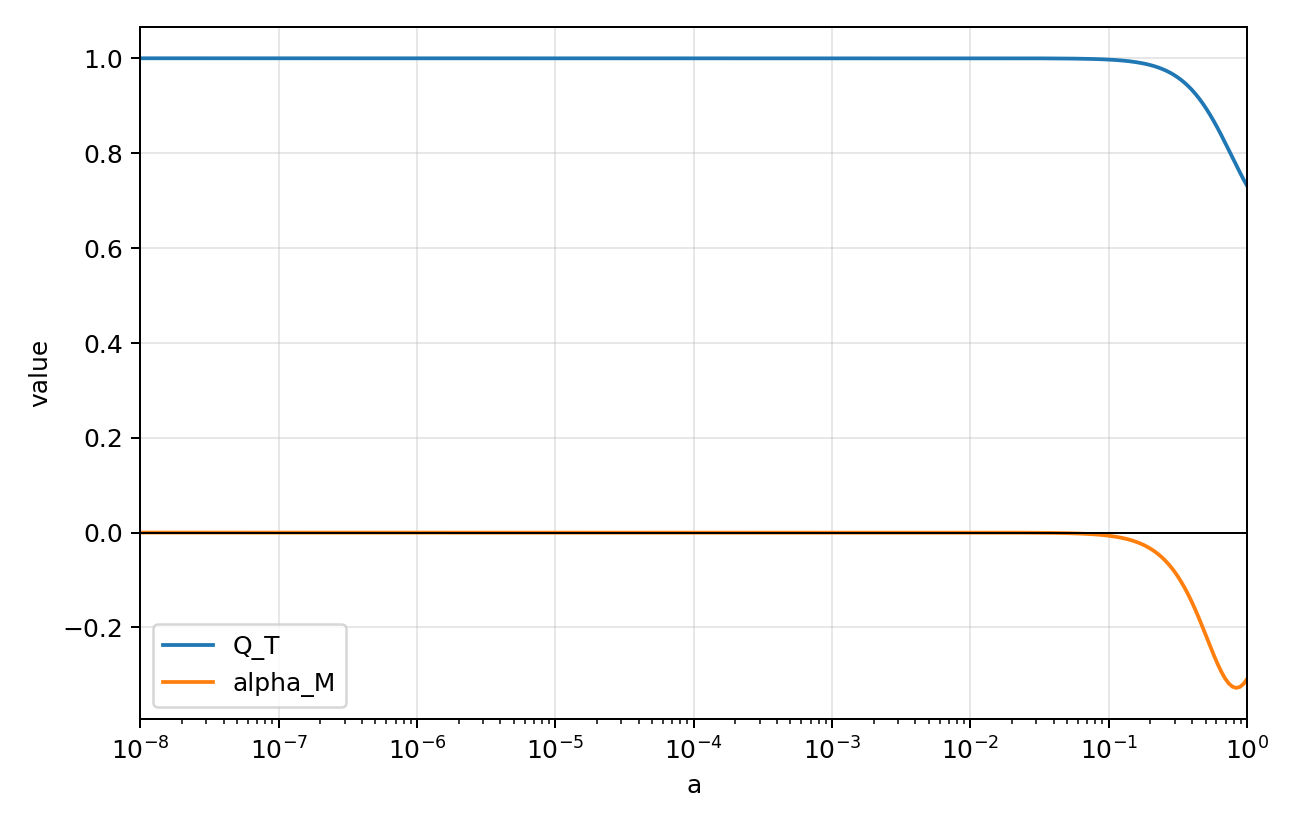
\includegraphics[width=0.82\textwidth]{download-2.png}
\caption{RFG-R tensor kinetic normalization \(Q_T\) and Planck-mass running
\(\alpha_M\) as functions of scale factor on the reference branch. The
positive \(Q_T\) curve verifies the tensor no-ghost condition, while the
quadratic tensor action gives \(c_T=1\) exactly. The plot defines the
standard-siren propagation prediction in Eq.~\eqref{eq:RFGR-siren}; it is not
itself a gravitational-wave or CMB likelihood evaluation. The generating
script is \RFGRepoNamed{scripts/generate\_outputs.py}{output generator}.}
\label{fig:rfgr-tensor-running}
\end{figure}
\FloatBarrier

The matter and CMB test is defined from the action derivatives, not from an
assumed quasi-static \(\mu(a,k)\). In particular,
\begin{align}
 \mathcal L_{{}^{(3)}R}&=Q_\epsilon,\\
 \mathcal L_{K_{ij}{}^{(3)}R}&=\frac{Q_{\epsilon,X}}{3H_0}\gamma^{ij},\\
\mathcal L_{K_{ij}}&=2Q_\epsilon(K^{ij}-K\gamma^{ij})
 +\left[\frac{Q_{\epsilon,X}}{3H_0}
 \left({}^{(3)}R+K_{mn}K^{mn}-K^2\right)
 +\frac{2H_0}{3}V_{\epsilon,X}\right]\gamma^{ij}.
 \label{eq:RFGR-ADM-derivatives}
\end{align}
\subsubsection{Exact ADM-to-extended-EFT map and solver boundary}
\label{sec:rfgr-extended-eft-map}

The preceding derivatives can be translated into a perturbation basis without
fitting a background surrogate.  The extended-EFT map of
Ref.~\cite{ExtendedEFTMap} uses the opposite extrinsic-curvature sign from the
convention of this manuscript.  Thus, for the map only,
\begin{equation}
 K_{ij}^{\rm map}=-K_{ij}^{\rm RFG},\qquad
 X=-\frac{K^{\rm map}}{3H_0}.
 \label{eq:RFGR-map-convention}
\end{equation}
With this explicit conversion, the exact RFG-R action gives
\begin{align}
 1+\Omega_{\rm EFT}&=Q_\epsilon,
 &\bar M_1^3&=-M_{\rm Pl}^2\dot Q_\epsilon,\nonumber\\
 \frac{\bar M_2^2}{M_{\rm Pl}^2}
 &=\frac{X^2Q_{\epsilon,XX}}{3}
   +\frac{4XQ_{\epsilon,X}}{3}-\frac{V_{\epsilon,XX}}9,
 &\bar M_3^2&=0,\nonumber\\
 \bar m_5&=-\frac{M_{\rm Pl}^2Q_{\epsilon,X}}{3H_0}.
 \label{eq:RFGR-extended-EFT-map}
\end{align}
In particular, the last coefficient multiplies
\begin{equation}
 \frac{\bar m_5}{2}\,\delta{}^{(3)}R\,\delta K
 =-\frac{M_{\rm Pl}^2Q_{\epsilon,X}}{6H_0}
 \,\delta{}^{(3)}R\,\delta K .
 \label{eq:RFGR-m5-operator}
\end{equation}
It is required by the \(Q_\epsilon(K){}^{(3)}R\) term in the action, hence
cannot consistently be set to zero.  The executable
\RFGRepoNamed{docs/extended\_eft\_mapping.md}{mapping note},
\RFGRepoNamed{scripts/extended\_eft\_mapping.py}{generator}, and
\RFGRepoNamed{generated/tables/extended\_eft\_mapping.csv}{CSV table}
are public and mutually linked.  On the published
mapping grid \(10^{-7}\leq a\leq1\), the independent validation gives
\(\min Q_\epsilon=0.7308038462\),
\(\max\lvert H_0\bar m_5/M_{\rm Pl}^2\rvert=0.1435712821\), a maximum
finite-difference error \(8.018\times10^{-7}\) for the second implicit
background derivative, and zero numerical error in the algebraic
\(\bar m_5\) identity.

\subsubsection{Executed pure-gravity extended-EFT scalar audit}
\label{sec:rfgr-extended-scalar-audit}

The scalar action must also be checked in the same operator basis before it
is handed to a Boltzmann hierarchy.  For the exact RFG-R map,
\(m_2^2=\lambda_i=\hat M^2=0\), while both \(\bar m_5\) and
\(W_7=-(\bar M_3^2+\bar M_2^2)/(2a^4)\) are nonzero.  Eliminating the
lapse and shift in the pure-gravity unitary-gauge action of
Ref.~\cite{ExtendedEFTMap} gives
\begin{equation}
 L_{\dot\zeta\dot\zeta}=
 \frac{(6a^2W_7+W_5)\bigl(3a^4W_4^2+2a^2W_1W_5\bigr)}
 {2a^2\bigl(W_4^2-4W_1W_7\bigr)} .
 \label{eq:RFGR-extended-scalar-kinetic}
\end{equation}
The full \(\bar m_5\) dependence is retained in the gradient and mixing
terms; its absence from Eq.~\eqref{eq:RFGR-extended-scalar-kinetic} is not a
licence to delete the operator.  The executable
\RFGRepoNamed{scripts/extended\_eft\_scalar\_stability.py}{scalar audit},
its independent
\RFGRepoNamed{scripts/validate\_extended\_eft\_scalar\_stability.py}{regression test},
the complete \RFGRepoNamed{docs/extended\_eft\_scalar\_audit.md}{derivation note},
and the machine-readable
\RFGRepoNamed{generated/tables/extended\_eft\_scalar\_stability.csv}{audit table}
are public.  On a \(49\times49\) logarithmic grid
\(10^{-7}\leq a\leq1\) and \(10^{-4}\leq k/H_0\leq10^5\), all
\(2401\) points satisfy
\begin{equation}
 \mathcal A_K:=6a^2W_7+W_5,\qquad
 \mathcal B_+:=3a^4W_4^2,\qquad
 \mathcal B_-:=2a^2W_1W_5,
 \label{eq:RFGR-extended-scalar-audit-definitions}
\end{equation}
\begin{equation}
 \min\bigl(W_4^2-4W_1W_7\bigr)=2.514017848646>0,
 \qquad
 \max\frac{|\mathcal A_K(\mathcal B_++\mathcal B_-)|}
 {|\mathcal A_K|\,(|\mathcal B_+|+|\mathcal B_-|)}
 =4.357\times10^{-16}.
 \label{eq:RFGR-extended-scalar-audit}
\end{equation}
Thus the pure-gravity scalar quadratic kinetic coefficient is degenerate to
the precision of the calculation; a standalone scalar sound speed is
undefined.  This is a pre-Boltzmann strong-coupling/constraint gate, not a
successful scalar-stability result.  It does \emph{not} by itself prove that
the physical matter-coupled theory is ill posed: matter sources the lapse and
shift constraints, and the separate one-canonical-scalar reduction below has
a different, nondegenerate sourced Hessian.  The decisive missing object is
therefore the complete photon--baryon--CDM--neutrino kinetic and gradient
matrix derived from the same action.

The audited public H-EFTCAMB source exposes the usual
\(\Omega,\gamma_1,\ldots,\gamma_6\) interface, but not the coefficient in
Eq.~\eqref{eq:RFGR-m5-operator}; the source-level audit is public in
\RFGRepoNamed{docs/backend\_capability\_audit.md}{the backend audit}. It therefore
cannot produce an exact RFG-R CMB, lensing, or matter spectrum without an
extension of its scalar equations and stability checks. Independently of that backend gap,
Eq.~\eqref{eq:RFGR-extended-scalar-audit} blocks a direct one-scalar EFT run.
This is a precise implementation boundary, not a negative data result and not
a licence to omit the operator.  The full kinetic Hessian must be obtained by
differentiating Eq.~\eqref{eq:RFGR-ADM-derivatives} after the physical matter
species are included. For every sampled cosmology, a full 3+1
Einstein--Boltzmann implementation must reject absent background roots,
\(Q_T\leq0\), ghosts, gradient instabilities, and singular constraint
matrices before computing
\(C_\ell^{TT,TE,EE}\), \(C_L^{\phi\phi}\), \(P(k,z)\),
\(f\sigma_8(z)\), and Eq.~\eqref{eq:RFGR-siren}. The intended joint
likelihood is
\begin{equation}
 \ln\mathcal L=\ln\mathcal L_{\rm Planck18}
 +\ln\mathcal L_{\rm lensing}+\ln\mathcal L_{\rm BAO}
 +\ln\mathcal L_{\rm SN}+\ln\mathcal L_{\rm RSD}
 +\ln\mathcal L_{\rm PPN}+\ln\mathcal L_{\rm GW}.
 \label{eq:RFGR-likelihood}
\end{equation}
The public calculation protocol, exact input/output contract, and deterministic
rejection conditions are supplied in
\RFGRepoNamed{docs/likelihood\_pipeline.md}{likelihood protocol}.  The installed Planck likelihood
components provide the data interface~\cite{PlanckLikelihood}; an RFG-R
solver must implement the physical multi-fluid reduction, retain
Eq.~\eqref{eq:RFGR-m5-operator}, reproduce its GR limit, and then be coupled
to that interface.  This is intentionally not a claim that the likelihood in
Eq.~\eqref{eq:RFGR-likelihood} has already been evaluated.

\subsubsection{Executed GR data-interface reference}
\label{sec:gr-planck-reference}

The ordinary radiation, recombination, lensing and data-interface machinery
has been exercised separately in GR using CAMB~\cite{CAMB} version 2.0.1 and
the Planck 2018 TT,TE,EE+lowE+lensing posterior-mean cosmological inputs
\(H_0=67.36\,{\rm km\,s^{-1}\,Mpc^{-1}}\),
\(\omega_b=0.02237\), \(\omega_c=0.1200\),
\(\tau=0.0544\), \(\ln(10^{10}A_s)=3.044\), \(n_s=0.9649\), and a
BBN-consistent helium fraction
\cite{Planck}. The pinned numerical reference gives
\(\sigma_8(0)=0.8110325278646\) together with reproducible lensed
\(TT\), \(TE\), \(EE\), lensing-potential, and linear-matter samples in
\RFGRepoNamed{generated/tables/gr\_camb\_reference.csv}{the GR CAMB CSV}.
The exact generator and regression test are
\RFGRepoNamed{scripts/gr\_reference\_camb.py}{the CAMB generator} and
\RFGRepoNamed{scripts/validate\_gr\_reference\_camb.py}{its regression test}.

The official Planck low-temperature, low-polarization and lensing components
were then evaluated at that fixed GR point. Their directly computed values are
\begin{equation}
 \ln\mathcal L_{\rm lowT}^{\rm GR}=-11.7117375873,\qquad
 \ln\mathcal L_{\rm lowE}^{\rm GR}=-198.063447867,\qquad
 \ln\mathcal L_{\rm lens}^{\rm GR}=-4.39556885539,
 \label{eq:gr-planck-lowell-components}
\end{equation}
or \(-2\ln\mathcal L_{\rm low\ell+lens}^{\rm GR}=428.341508619\).
The machine result, execution script and regression test are public in
\RFGRepoNamed{generated/tables/gr\_planck\_2018\_lowell\_lensing.csv}{the likelihood CSV},
\RFGRepoNamed{scripts/gr\_planck\_lowell\_lensing.py}{the likelihood script}, and
\RFGRepoNamed{scripts/validate\_gr\_planck\_lowell\_lensing.py}{its regression test}.
The high-\(\ell\) Plik package is installed but deliberately not evaluated
with guessed foreground and calibration parameters: those form part of a
documented joint fit. This reference validates the public data path only. It
sets \(\bar m_5=0\) because CAMB is GR, and is therefore neither an RFG-R
likelihood nor evidence for RFG-R against \(\Lambda\)CDM; see
\RFGRepoNamed{docs/planck\_data\_reference.md}{the data-reference note}.

\subsubsection{Exact photon--baryon--CDM--neutrino reduction}
\label{sec:rfgr-multifluid-reduction}

The physical sourced reduction is obtained directly from the RFG-R action,
rather than by adding a phenomenological \(\mu(a,k)\), a sound-speed closure,
or a quasi-static approximation.  For each barotropic monopole--dipole
matter source, the starting point is the Sorkin--Schutz action
\cite{DeFeliceMatter}
\begin{equation}
 S_i=-\int\dd^4x\left[\sqrt{-g}\,\rho_i(n_i)
       +J_i^\mu\partial_\mu\ell_i\right],
 \qquad p_i=n_i\rho_{i,n}-\rho_i .
 \label{eq:RFGR-Sorkin-Schutz}
\end{equation}
Let \(s=k^2\psi/a^2\), and define the physical and auxiliary vectors
\begin{equation}
 \mathbf q=(\zeta,\delta_b,\delta_c,\delta_\gamma,\delta_\nu)^T,
 \qquad
 \mathbf x=(\alpha,s,v_b,v_c,v_\gamma,v_\nu)^T .
 \label{eq:RFGR-multifluid-variables}
\end{equation}
The exact finite scalar density, retaining the complete extended-EFT gravity
action, is
\begin{equation}
 L^{(2)}=\frac12\dot{\mathbf q}^{T}K_0\dot{\mathbf q}
 +\mathbf x^TC\dot{\mathbf q}+\frac12\mathbf x^TA\mathbf x
 +\mathbf x^TD\mathbf q+\frac12\mathbf q^TM_0\mathbf q .
 \label{eq:RFGR-multifluid-block-action}
\end{equation}
Its nonzero entries are
\begin{align}
 (K_0)_{\zeta\zeta}&=-3a^2W_5,&
 C_{\alpha\zeta}&=-3a^2W_4,& C_{s\zeta}&=-a^2W_5,\nonumber\\
 A_{\alpha\alpha}&=2W_1,& A_{\alpha s}&=-a^2W_4,&
 A_{ss}&=2a^4W_7,\nonumber\\
 D_{\alpha\zeta}&=-W_6k^2,&
 D_{s\zeta}&=-2\bar m_5\frac{k^2}{a^2},&
 (M_0)_{\zeta\zeta}&=-2W_0k^2,\nonumber\\
 C_{v_i\zeta}&=-3\rho_i(1+w_i),&
 C_{v_i\delta_i}&=-\rho_i,&
 A_{sv_i}&=-\rho_i(1+w_i),\nonumber\\
 A_{v_iv_i}&=-\rho_i(1+w_i)\frac{k^2}{a^2},&
 D_{\alpha\delta_i}&=-\rho_i,&
 (M_0)_{\delta_i\delta_i}&=-\frac{\rho_iw_i}{1+w_i}.
 \label{eq:RFGR-multifluid-blocks}
\end{align}
Here \(i=b,c,\gamma,\nu\), with \(w_{b,c}=0\) and \(w_{\gamma,\nu}=1/3\)
only in the density--momentum constraint rows.  It is not a closure of the
photon or neutrino hierarchy.

Varying \(\alpha\) and \(s\) gives the exact sourced lapse--shift system
\begin{align}
 2W_1\alpha-a^2W_4s-3a^2W_4\dot\zeta-W_6k^2\zeta
 -\sum_i\rho_i\delta_i&=0,\nonumber\\
 -a^2W_4\alpha+2a^4W_7s-a^2W_5\dot\zeta
 -2\bar m_5\frac{k^2}{a^2}\zeta
 -\sum_i\rho_i(1+w_i)v_i&=0.
 \label{eq:RFGR-multifluid-constraints}
\end{align}
The determinant is the analytic identity
\begin{equation}
 \det A_{(\alpha,s)}=-a^4\left(W_4^2-4W_1W_7\right),
 \label{eq:RFGR-multifluid-constraint-determinant}
\end{equation}
and eliminating all auxiliary variables yields the complete finite Schur
reduction
\begin{equation}
 K=K_0-C^TA^{-1}C,\qquad
 B=-C^TA^{-1}D,\qquad
 M=M_0-D^TA^{-1}D.
 \label{eq:RFGR-multifluid-Schur}
\end{equation}

The photon and neutrino anisotropic-stress sectors are not discarded.  In the
same spatial gauge, \(\chi=-\psi\), their exact massless Boltzmann hierarchy
is \cite{HwangNoh}
\begin{equation}
 \dot\Theta_\ell=\frac{k}{a}\left[
 \frac{\Theta_{\ell-1}}{2\ell-1}
 -\frac{\Theta_{\ell+1}}{2\ell+3}\right]+M_\ell+C_\ell,
 \label{eq:RFGR-massless-hierarchy}
\end{equation}
where the \(\ell=0\) streaming term is \(-k\Theta_1/(3a)\), and
\begin{equation}
 M_0=-\dot\zeta-\frac{s}{3},\qquad
 M_1=\frac{k}{a}\alpha,\qquad M_2=\frac{2s}{3},
 \qquad M_{\ell\ge3}=0 .
 \label{eq:RFGR-hierarchy-metric-sources}
\end{equation}
For photons \(C_0=0\), \(C_1=\dot\tau(v_b-\Theta_1)\),
\(C_2=\dot\tau(P-\Theta_2)\), \(C_{\ell\ge3}=-\dot\tau\Theta_\ell\),
where
\begin{equation}
 P=\frac{\Theta_2-\sqrt6E_2}{10},\qquad
 \dot\tau=n_e x_e\sigma_T\ge0 .
 \label{eq:RFGR-Thomson}
\end{equation}
The exact scalar polarization hierarchy, for \(\ell\ge2\), is
\begin{equation}
 \dot E_\ell=\frac{k}{a}\left[
 \frac{\sqrt{\ell^2-4}}{2\ell-1}E_{\ell-1}
 -\frac{\sqrt{(\ell+1)^2-4}}{2\ell+3}E_{\ell+1}\right]
 -\dot\tau\left(E_\ell+\sqrt6P\,\delta_{\ell2}\right),
 \qquad B_\ell^{(0)}=0 .
 \label{eq:RFGR-polarization-hierarchy}
\end{equation}
For a collisionless massless neutrino, \(C_\ell=0\) at every \(\ell\).  Thus
Eqs.~\eqref{eq:RFGR-massless-hierarchy}--\eqref{eq:RFGR-polarization-hierarchy}
are an infinite hierarchy, not a fluid approximation or a prescribed
\(\ell_{\max}\) terminal closure.  Their first moments obey
\(\delta_{\gamma,\nu}=4\Theta_{\gamma,\nu,0}\),
\(v_{\gamma,\nu}=\Theta_{\gamma,\nu,1}\), and
\(\pi_{\gamma,\nu}/\rho_{\gamma,\nu}=4\Theta_{\gamma,\nu,2}/5\), which
matches the constraint action above exactly.

For a massive neutrino no massless substitution is made.  With
\(\epsilon(q,a)=\sqrt{q^2+a^2m_\nu^2}\), the collisionless phase-space
equation is
\begin{equation}
 \delta f'=-\frac{q}{\epsilon}\mathcal D_\gamma\delta f
 +q\frac{\partial f_0}{\partial q}
 \left[\frac{\epsilon}{q}A_{,\alpha}\gamma^\alpha
 +(B_{\alpha|\beta}+C'_{\alpha\beta})\gamma^\alpha\gamma^\beta\right].
 \label{eq:RFGR-massive-neutrino}
\end{equation}
The density, momentum and anisotropic stress are the corresponding exact
momentum integrals with the \(\epsilon\) weights; no effective equation of
state is inserted.

The executable derivation is
\RFGRepoNamed{docs/photon\_baryon\_cdm\_neutrino\_reduction.md}{the full reduction note};
the matrix/hierarchy implementation is
\RFGRepoNamed{scripts/multifluid\_reduction.py}{the reduction module}, and
the independent validation is
\RFGRepoNamed{scripts/validate\_multifluid\_reduction.py}{the audit script}.
The GR test is performed with rational arithmetic and gives
\(\operatorname{rank}K=4\) exactly.  The separate 425-point RFG-R audit uses
the published Planck 2018 Table~2 species split solely as a documented input
record~\cite{Planck}: it gives a maximum constraint-determinant residual
\(4.148\times10^{-15}\) and inertia
\((n_+,n_-,n_0)=(4,0,1)\) at every point.  Those values are not an RFG-R fit,
and neither this reduction nor the audit evaluates a CMB likelihood.  The
machine table is
\RFGRepoNamed{generated/tables/multifluid\_core\_audit.csv}{multifluid audit CSV}.

\subsubsection{Spatial metric equations and exact DAE closure}
\label{sec:rfgr-dae-closure}

The lapse--shift reduction alone is not a metric evolution law. To obtain the
remaining scalar equation, the traceless spatial deformation must be retained
before the spatial gauge is imposed:
\begin{equation}
 \gamma_{ij}=a^2e^{2\zeta}\exp(2D_{ij}E),\qquad
 D_{ij}=\partial_i\partial_j-\frac13\delta_{ij}\partial^2 .
 \label{eq:RFGR-traceless-metric}
\end{equation}
Direct variation of the original ADM action with respect to \(E\), followed
only then by \(E=0\), gives in units \(H_0=M_{\rm Pl}=1\), with
\(s=k^2\beta/a^2\),
\begin{align}
 \dot s={}&-\left(3H+\frac{\dot Q}{Q}
 +\frac{Q_Xk^2}{3Qa^2}\right)s
 -\frac{k^2}{a^2}(\alpha+\zeta)
 +\frac{Q_Xk^2}{Qa^2}(H\alpha-\dot\zeta)
 -\frac{\Pi}{Q} .
 \label{eq:RFGR-traceless-evolution}
\end{align}
Here \(\Pi\) is the total scalar anisotropic stress; for each massless
kinetic species \(\Pi_i=4\rho_i\Theta_{i2}/5\). The independently checked
Einstein--Hilbert limit of Eq.~\eqref{eq:RFGR-traceless-evolution} is
\begin{equation}
 \dot s=-3Hs-\frac{k^2}{a^2}(\alpha+\zeta)-\Pi .
 \label{eq:RFGR-traceless-GR}
\end{equation}
The executable variation performs the lapse, shift, trace, and traceless GR
regressions directly from the ADM density:
\RFGRepoNamed{scripts/derive\_spatial\_traceless\_equation.py}{spatial-variation script}.

The exact Schur reduction in Eq.~\eqref{eq:RFGR-multifluid-Schur} has one
null kinetic direction. It becomes explicit under the invertible field
redefinition
\begin{equation}
 \Delta_i=\delta_i+3(1+w_i)\zeta,
 \qquad
 \mathbf y=(\zeta,\Delta_b,\Delta_c,\Delta_\gamma,\Delta_\nu)^T.
 \label{eq:RFGR-Delta-definition}
\end{equation}
Writing the reduced density as
\begin{equation}
 L_{\rm red}=\frac12\dot{\mathbf y}^{T}K_\Delta\dot{\mathbf y}
 +\dot{\mathbf y}^{T}B_\Delta\mathbf y
 +\frac12\mathbf y^TM_\Delta\mathbf y,
 \label{eq:RFGR-DAE-density}
\end{equation}
the exact identities are
\begin{equation}
 (K_\Delta)_{0j}=0,\qquad B_\Delta=B_\Delta^T.
 \label{eq:RFGR-DAE-identities}
\end{equation}
Thus \(\zeta\) is not an omitted propagating mode and no temporal gauge has
been selected: its Euler equation is the algebraic curvature constraint
\begin{equation}
 \mu_\zeta(a,k)\zeta+
 \sum_i\left[(M_\Delta)_{0i}-(\dot B_\Delta)_{0i}\right]\Delta_i=0,
 \qquad
 \mu_\zeta=(M_\Delta)_{00}-(\dot B_\Delta)_{00}.
 \label{eq:RFGR-curvature-constraint}
\end{equation}
All derivatives in Eq.~\eqref{eq:RFGR-curvature-constraint} are analytic
derivatives of the RFG-R action, including \(Q_{XXX}\), \(V_{XXX}\), and
\(\dot W_i\); no tabulated-background finite difference enters the result.

This calculation closes the finite DAE question, and it gives a negative
viability result for the stated reference branch. On a 49-point logarithmic
grid in \(a\in[10^{-7},1]\), \(24\) scale factors have a finite positive root
of \(\mu_\zeta\). In particular,
\begin{equation}
 \left.\frac{k}{H_0}\right|_{a=1,\ \mu_\zeta=0}=2.51545672221 .
 \label{eq:RFGR-curvature-root}
\end{equation}
At this surface Eq.~\eqref{eq:RFGR-curvature-constraint} ceases to determine
\(\zeta\). The independently validated residuals are
\(\max_j|(K_\Delta)_{0j}|/\max|K_\Delta|=5.923\times10^{-15}\) and
\(\max|B_\Delta-B_\Delta^T|/\max|B_\Delta|=1.360\times10^{-16}\), so the
zero is not a hierarchy truncation or a loss of numerical precision. The
derivation, independent regression, and root table are public in
\RFGRepoNamed{docs/rfg\_dae\_closure.md}{the DAE derivation},
\RFGRepoNamed{scripts/rfg\_dae\_closure.py}{the DAE generator},
\RFGRepoNamed{scripts/validate\_rfg\_dae\_closure.py}{its independent validator}, and
\RFGRepoNamed{generated/tables/multifluid\_dae\_closure.csv}{the root table}.

Therefore the published RFG-R reference action does not define globally
regular linear transfer functions. No CMB, lensing, matter, or joint
likelihood value for that branch may be obtained by forcing an integration
through Eq.~\eqref{eq:RFGR-curvature-root}. A modified action would be a new
theory and would require a fresh derivation and validation.

\subsubsection{RFG-R\texorpdfstring{\(\Xi\)}{Xi}: background-preserving foliation completion}
\label{sec:rfgr-xi-completion}

The singularity in Eq.~\eqref{eq:RFGR-curvature-constraint} is an internal
property of the reference action, not a request to revert to \(\Lambda\)CDM.
The minimal background-preserving R-Universe extension considered here is a
new action,
\begin{equation}
 S_{\Xi}=S_{\rm cos}+
 \frac{\mpl^2}{2}\int\dd^4x\,N\sqrt{\gamma}\,
 \Xi\left({}^{(3)}R+\sigma_{ij}\sigma^{ij}\right),
 \qquad \Xi=\text{constant},
 \label{eq:RFGR-Xi-action}
\end{equation}
where \(\sigma_{ij}=K_{ij}-K\gamma_{ij}/3\). Both terms in
Eq.~\eqref{eq:RFGR-Xi-action} vanish on a spatially flat FLRW background.
The reconstructed R-Universe Friedmann equation
\eqref{eq:RFGR-background} is therefore exactly unchanged. The same term
adds equally to the tensor kinetic and gradient coefficients,
\begin{equation}
 Q_T^{\Xi}=Q_\epsilon+\Xi,\qquad c_T^2=1.
 \label{eq:RFGR-Xi-tensor}
\end{equation}
The existing smooth Weyl matching rule multiplies the entire cosmological
Lagrangian, including Eq.~\eqref{eq:RFGR-Xi-action}; it remains exactly GR in
the local constant-switch domain.

For a real scalar Fourier mode, direct expansion of the ADM action gives
\begin{equation}
 \frac{\Delta L_{\Xi}^{(2)}}{a^3}
 =\Xi\left[
 2\frac{k^2}{a^2}\alpha\zeta
 +\frac{k^2}{a^2}\zeta^2+\frac{s^2}{3}\right].
 \label{eq:RFGR-Xi-quadratic}
\end{equation}
Thus the finite matrices of Eq.~\eqref{eq:RFGR-multifluid-block-action} are
modified without a fitted background function:
\begin{equation}
 \Delta A_{ss}=\frac{2\Xi}{3},\qquad
 \Delta D_{\alpha\zeta}=
 \Delta(M_0)_{\zeta\zeta}=2\Xi\frac{k^2}{a^2},
 \qquad
 \partial_t\Delta D_{\alpha\zeta}
 =\partial_t\Delta(M_0)_{\zeta\zeta}
 =-2H\Delta D_{\alpha\zeta}.
 \label{eq:RFGR-Xi-matrices}
\end{equation}
Equations~\eqref{eq:RFGR-Xi-action}--\eqref{eq:RFGR-Xi-matrices} define
RFG-R\(\Xi\), not a reinterpretation of the singular reference action.
Keeping the scalar traceless metric mode until after variation gives the
following exact additions to the lapse, shift, trace, and traceless Euler
residuals:
\begin{align}
 \Delta\mathcal E_\alpha&=2\Xi ak^2\zeta,&
 \Delta\mathcal E_\beta&=\frac{2\Xi\beta k^4}{3a}, \notag\\
 \Delta\mathcal E_\zeta&=-2\Xi ak^2(\alpha+\zeta),&
 \Delta\mathcal E_E&=-\frac{2\Xi ak^4}{3}
 \left(H\beta+\alpha+\dot\beta+\zeta\right).
 \label{eq:RFGR-Xi-metric-residuals}
\end{align}
Thus this is not an Einstein-equation substitution. In the gauge
\(s=k^2\beta/a^2\), the directly varied traceless equation is
\begin{align}
 \dot s={}&-\left[3H+\frac{\dot Q_\epsilon}{Q_\epsilon+\Xi}
 +\frac{Q_{\epsilon,X}}{3(Q_\epsilon+\Xi)}\frac{k^2}{a^2}\right]s
 -\frac{k^2}{a^2}(\alpha+\zeta) \notag\\
 &+\frac{Q_{\epsilon,X}}{Q_\epsilon+\Xi}\frac{k^2}{a^2}
 \left(H\alpha-\dot\zeta\right)-\frac{\Pi}{Q_\epsilon+\Xi}.
 \label{eq:RFGR-Xi-traceless-evolution}
\end{align}
Here \(\Pi\) is the total kinetic anisotropic stress. The symbolic regression
of all four residuals and the executable form of
Eq.~\eqref{eq:RFGR-Xi-traceless-evolution} are in
\RFGRepoNamed{scripts/validate\_rfg\_xi\_metric\_equations.py}{the RFG-RXi metric-equation test}.

The constant \(\Xi\) is a new dimensionless EFT coefficient, not a fitted
cosmological parameter in this work. For the unfitted normalization benchmark
\(\Xi=1\), the exact
multi-fluid DAE audit scans \(49\) values of
\(a\in[10^{-7},1]\) and \(81\) values of
\(k/H_0\in[10^{-4},10^6]\). It finds no sampled
\(\mu_\zeta\) root, \(\min Q_T^\Xi=1.736101654462\), and
\(\min|\det A_{(\alpha,s)}|=5.991445560907\). The four-dimensional material
kinetic block has inertia \((4,0,0)\) at every audited point. The direct
symbolic identity, audit, and table are reproducible from
\RFGRepoNamed{docs/rfg\_xi\_completion.md}{the RFG-RXi derivation},
\RFGRepoNamed{scripts/rfg\_xi\_completion.py}{the RFG-RXi audit},
\RFGRepoNamed{scripts/validate\_rfg\_xi\_completion.py}{its regression test},
\RFGRepoNamed{scripts/validate\_rfg\_xi\_metric\_equations.py}{the exact metric-equation regression}, and
\RFGRepoNamed{generated/tables/rfg\_xi\_completion\_audit.csv}{the audit table}.
An extended audit samples \(193\) values of
\(a\in[10^{-8},1]\) and \(601\) values of
\(k/H_0\in[10^{-5},10^7]\) for each of \(\Xi=1,2\). It finds no sampled
curvature-constraint root, retains positive \(Q_T^\Xi\) and a nonsingular
lapse--shift block, and has \(\min|\mu_\zeta|_{\rm normalized}=1\) on that
declared domain. Its generator, independent check, and machine table are
\RFGRepoNamed{scripts/rfg\_xi\_dense\_dae\_audit.py}{the extended DAE audit},
\RFGRepoNamed{scripts/validate\_rfg\_xi\_dense\_dae\_audit.py}{its regression test}, and
\RFGRepoNamed{generated/tables/rfg\_xi\_dense\_dae\_audit.csv}{the extended audit table}.

\paragraph{Directly evaluated RFG-R\(\Xi\) factors.}
The local Weyl switch is exactly zero in the Solar-System matching domain, so
the \(\Xi\) operator is absent there and the action gives
\begin{equation}
 \gamma_{\rm PPN}=\beta_{\rm PPN}=1,\qquad
 \alpha_1=\alpha_2=0,\qquad
 -2\ln\mathcal L_{\rm Cassini}=0.8336483932 .
 \label{eq:RFGR-Xi-Cassini}
\end{equation}
This is a directly evaluated Cassini data factor for both \(\Xi=1\) and
\(\Xi=2\), not a surrogate for a CMB likelihood. The corresponding exact
tensor prediction is
\begin{equation}
 Q_T^\Xi(a)=Q_\epsilon(a)+\Xi,\qquad c_T^2=1,\qquad
 \frac{d_L^{\rm GW}}{d_L^{\rm EM}}=
 \left[\frac{Q_T^\Xi(1)}{Q_T^\Xi(a)}\right]^{1/2}.
 \label{eq:RFGR-Xi-direct-observables}
\end{equation}
At the Planck-recorded background input, the action yields
\(d_L^{\rm GW}/d_L^{\rm EM}=0.9565968846\) at \(z\simeq1\) for \(\Xi=1\),
and \(0.9717969466\) for \(\Xi=2\). The full grid, the exact Cassini factor,
and the linked DAE diagnostics are public in
\RFGRepoNamed{docs/rfg\_xi\_validated\_factors.md}{the direct-factor note},
\RFGRepoNamed{scripts/rfg\_xi\_observables.py}{the observable generator},
\RFGRepoNamed{scripts/validate\_rfg\_xi\_observables.py}{its regression test},
\RFGRepoNamed{generated/tables/rfg\_xi\_observables.csv}{the observable grid}, and
\RFGRepoNamed{generated/tables/rfg\_xi\_validated\_factors.csv}{the factor summary}.

This is a viability gate for a distinct R-Universe action, not a CMB fit,
posterior, or a proof of nonlinear health. Initial conditions, the complete
Boltzmann integration, gradient and nonlinear stability, and an observational
likelihood remain to be calculated from Eq.~\eqref{eq:RFGR-Xi-action}.

\subsection{Exact canonical-scalar reference reduction}
\label{sec:rfgr-canonical-scalar}

The first sourced scalar check for the regular RFG-R action can be completed
without a quasi-static approximation.  It is deliberately narrower than a
cosmological matter calculation: the matter sector is one minimally coupled,
canonical scalar \(\phi\), and scalar-field comoving gauge
\(\delta\phi=0\) is used.  Thus the result tests the physical scalar mode
and the sourced lapse--shift constraints, but it is not a replacement for the
photon, baryon, cold-dark-matter and neutrino hierarchies required by the CMB
likelihood.

Put \(p=k^2/a^2\), \(y=p\beta\),
\(m=\dot\phi^2/\mpl^2\), and
\(D=-F_{\epsilon,XX}/3\), where \(F_\epsilon\) is the RFG-R ADM
Lagrangian evaluated on the background.  After including the complete
intrinsic-curvature contribution and the canonical scalar action, the
nondynamical variables \(\mathbf{x}=(\alpha,y)^T\) have Hessian
\begin{equation}
 H_{(\alpha,y)}=
 \begin{pmatrix}
  2(-3DH^2+m) & 2DH\\
  2DH & 2(-D+2Q_\epsilon)/3
 \end{pmatrix},
 \qquad
 \det H_{(\alpha,y)}=-\frac{4}{3}\Delta,
 \label{eq:RFGR-canonical-hessian}
\end{equation}
with the exact constraint discriminant
\begin{equation}
 \Delta=6DH^2Q_\epsilon+(D-2Q_\epsilon)m.
 \label{eq:RFGR-canonical-delta}
\end{equation}
The lapse and shift constraints are invertible precisely where
\(\Delta\ne0\).  Eliminating them by the Schur complement gives
\begin{equation}
 S_{\rm red}^{(2)}=\frac{\mpl^2}{2}\int\dd t\,\dd^3k\,a^3
 \left[K\dot\zeta^2+
 \left(C_0+C_1p+C_2p^2\right)\zeta^2\right],
 \qquad
 K=\frac{6DQ_\epsilon m}
 {6DH^2Q_\epsilon+(D-2Q_\epsilon)m}.
 \label{eq:RFGR-canonical-reduced}
\end{equation}
Here the mixed \(\zeta\dot\zeta\) term has been integrated by parts;
the exact algebraic expressions for \(C_0,C_1,C_2\) follow from the same
matrix reduction.  The physical low-gradient and \(k^4\) coefficients are
\begin{equation}
 G_1=-C_1,\qquad G_2=-C_2,\qquad
 c_{s,\rm low}^2=\frac{G_1}{K}\quad(K>0).
 \label{eq:RFGR-canonical-gradients}
\end{equation}
Equations~\eqref{eq:RFGR-canonical-hessian}--\eqref{eq:RFGR-canonical-gradients}
are exact for the stated one-field system.  The full derivation, including
the curvature term needed to recover the GR sound speed, is available in
\RFGRepoNamed{docs/canonical\_scalar\_reduction.md}{canonical-scalar derivation}; the executable
calculation is \RFGRepoNamed{scripts/canonical\_scalar.py}{canonical-scalar solver} and its machine
readable reference output is
\RFGRepoNamed{generated/tables/canonical\_scalar\_reference.csv}{reference CSV}.

Two checks are built into the calculation.  First, GR coupled to a massless
canonical (stiff) scalar gives exactly \(K=6\) and
\(c_{s,\rm low}^2=1\).  Second, on the regular RFG-R reference branch
\(\theta=1.6\), \(\Omega_{\phi0}=0.30\), \(\Omega_{R0}=0.70\), and
\(0.03\le a\le1\), the numerical scan returns
\begin{equation}
\begin{aligned}
 \min\Delta&=8.006769231,\qquad
 \min K=1.695411575,\\
 \min G_1&=0.5673484131,\qquad
 c_{s,\rm low}^2(a=1)=0.3346375721.
\end{aligned}
 \label{eq:RFGR-canonical-reference}
\end{equation}
The calculated \(G_2\) is non-negative to numerical precision; its minimum
is \(-4.7\times10^{-10}\), a floating-point residual around the GR-asymptotic
value zero.  This is a reproducible internal viability gate for the specified
one-field branch, not a multi-fluid stability theorem or a CMB data result.

\subsection{Reproducibility and public links}

The self-contained supplement distributed beside this \LaTeX{} source is
\RFGRepoNamed{README.md}{README}. Its calculation manifest is
\RFGRepoNamed{CALCULATION\_MANIFEST.md}{calculation manifest}; the executable validation command is
\texttt{bash r\_universe\_completion/scripts/run\_all.sh}. The permanent
public counterparts are linked directly from the paper:
\RFGRepoNamed{docs/completion\_derivation.md}{completion derivation},
\RFGRepoNamed{docs/likelihood\_pipeline.md}{likelihood protocol},
\RFGRepoNamed{docs/photon\_baryon\_cdm\_neutrino\_reduction.md}{multifluid reduction}, and
\RFGRepoNamed{docs/canonical\_scalar\_reduction.md}{canonical-scalar derivation},
\RFGRepoNamed{scripts/multifluid\_reduction.py}{multifluid module},
\RFGRepoNamed{scripts/validate\_multifluid\_reduction.py}{multifluid audit},
\RFGRepoNamed{scripts/canonical\_scalar.py}{canonical-scalar solver}, and
\RFGRepoNamed{scripts/validate\_completion.py}{validation script}. The repository directory also
contains the exact source of the manuscript, generated tables, figures, and
the \RFGRepoNamed{paper/R\_Universe\_RFG\_R\_Completion.pdf}{standalone RFG-R completion article}.

\section{Quadratic scalar geometry and constraint kernel}
\label{sec:quadratic_scalar}

This section develops the scalar perturbation sector directly from the RFG
action.  No auxiliary scalar field and no scalar--tensor closure assumption is introduced.
The only inputs are the preferred-foliation ADM variables and the functions
\(Q(X)\) and \(V(X)\) already fixed by the homogeneous reconstruction.

We use
\begin{equation}
N=1+\alpha,\qquad
N_i=\partial_i\beta,\qquad
\gamma_{ij}=a^2 e^{2\zeta}\delta_{ij},
\label{eq:scalar_adm_param}
\end{equation}
and
\begin{equation}
K_{ij}=\frac{1}{2N}
\left(\dot\gamma_{ij}-D_iN_j-D_jN_i\right),
\qquad
X=\frac{K}{3H_0}.
\label{eq:scalar_K_definition}
\end{equation}
All perturbative orders below refer to powers of
\(\alpha,\beta,\zeta\).

\subsection{Exact measure and intrinsic curvature}

\begin{lemma}[Measure expansion]
For the parametrization \eqref{eq:scalar_adm_param},
\begin{equation}
\sqrt{\gamma}=a^3e^{3\zeta},
\end{equation}
and hence
\begin{equation}
N\sqrt{\gamma}
=
a^3\left[
1+\alpha+3\zeta+3\alpha\zeta+\frac{9}{2}\zeta^2
\right]+O(3).
\label{eq:measure_second_order}
\end{equation}
\end{lemma}

\begin{proof}
The determinant is
\(\det\gamma_{ij}=a^6e^{6\zeta}\).  Taking its positive square root and
expanding the exponential gives \eqref{eq:measure_second_order}.  Because
\(N=1+\alpha\) is used as the perturbation variable, no independent
\(\alpha^2\) term occurs in the measure.
\end{proof}

\begin{lemma}[Intrinsic curvature expansion]
For \(\gamma_{ij}=a^2e^{2\zeta}\delta_{ij}\),
\begin{equation}
{}^{(3)}R
=
\frac{e^{-2\zeta}}{a^2}
\left[-4\partial^2\zeta-2(\partial\zeta)^2\right].
\label{eq:exact_3curvature}
\end{equation}
Consequently,
\begin{align}
R^{(1)}&=-\frac{4}{a^2}\partial^2\zeta,
\\
R^{(2)}&=
\frac{1}{a^2}
\left[
8\zeta\,\partial^2\zeta-2(\partial\zeta)^2
\right].
\label{eq:3curvature_orders}
\end{align}
\end{lemma}

\subsection{Extrinsic curvature and the relational perturbation}

Define
\begin{equation}
b\equiv\frac{\partial^2\beta}{a^2}.
\end{equation}
Direct contraction of \eqref{eq:scalar_K_definition} gives the exact trace
\begin{equation}
K=
\frac{1}{1+\alpha}
\left[
3(H+\dot\zeta)
-\frac{e^{-2\zeta}}{a^2}
\left(\partial^2\beta+\partial_i\zeta\,\partial_i\beta\right)
\right].
\label{eq:exact_K_scalar}
\end{equation}
Writing
\begin{equation}
K=3H+\delta K_1+\delta K_2+O(3),
\end{equation}
one obtains
\begin{align}
\delta K_1
&=
3\dot\zeta-3H\alpha-b,
\label{eq:deltaK1}
\\
\delta K_2
&=
3H\alpha^2-3\alpha\dot\zeta+\alpha b
-\frac{1}{a^2}\partial_i\zeta\,\partial_i\beta
+\frac{2\zeta}{a^2}\partial^2\beta.
\label{eq:deltaK2}
\end{align}
For a Fourier mode, let
\begin{equation}
u\equiv\dot\zeta-H\alpha,
\qquad
y\equiv\frac{k^2}{a^2}\beta.
\label{eq:u_y_def}
\end{equation}
Since \(b=-y\), the linear relational perturbation becomes
\begin{equation}
\boxed{\delta K_1=3u+y},
\qquad
\delta X_1=\frac{3u+y}{3H_0}.
\label{eq:deltaK1_uy}
\end{equation}

\subsection{Trace--shear decomposition}

Introduce the shear
\begin{equation}
\sigma_{ij}=K_{ij}-\frac{1}{3}K\gamma_{ij}.
\end{equation}
The exact algebraic identity
\begin{equation}
K_{ij}K^{ij}-K^2
=
\sigma_{ij}\sigma^{ij}-\frac{2}{3}K^2
\label{eq:trace_shear_identity}
\end{equation}
separates the trace response from the shift shear.  Since the background shear
vanishes, only its linear part is required at quadratic order:
\begin{equation}
\sigma_{ij}\sigma^{ij}
=
\frac{1}{a^4}
\left[
(\partial_i\partial_j\beta)^2
-\frac{1}{3}(\partial^2\beta)^2
\right]+O(3).
\label{eq:shear_square_position}
\end{equation}
For one Fourier mode this reduces to
\begin{equation}
\boxed{
\sigma_{ij}\sigma^{ij}=\frac{2}{3}y^2
}.
\label{eq:shear_square_fourier}
\end{equation}

\subsection{Equivalent scalar kernel of the RFG action}

Define
\begin{equation}
F(X)\equiv -3X^2Q(X)+V(X).
\label{eq:F_definition}
\end{equation}
Using \(K=3H_0X\) and \eqref{eq:trace_shear_identity}, the gravitational
action is identically rewritten as
\begin{equation}
S_g=
\frac{M_{\rm Pl}^2}{2}
\int dt\,d^3x\,N\sqrt{\gamma}
\left[
Q(X)\,{}^{(3)}R
+Q(X)\sigma_{ij}\sigma^{ij}
+2H_0^2F(X)
\right].
\label{eq:RFG_trace_shear_action}
\end{equation}
Equation \eqref{eq:RFG_trace_shear_action} is not an additional assumption; it is an
algebraically equivalent form of the original RFG action.

Let
\begin{equation}
\bar X=\frac{H}{H_0},
\qquad
\delta X_1=\frac{\delta K_1}{3H_0},
\qquad
\delta X_2=\frac{\delta K_2}{3H_0},
\end{equation}
and evaluate \(Q,F\) and their derivatives at \(\bar X\).  Before use of the
background equations or integrations by parts, the quadratic gravitational
density is
\begin{align}
\frac{\mathcal L_g^{(2)}}{(M_{\rm Pl}^2/2)a^3}
={}&
Q R^{(2)}
+\left[Q(\alpha+3\zeta)+Q_{,X}\delta X_1\right]R^{(1)}
+Q\,\sigma_{ij}\sigma^{ij}
\nonumber\\
&+2H_0^2
\Bigg[
F\left(3\alpha\zeta+\frac{9}{2}\zeta^2\right)
+F_{,X}
\left(
\delta X_2+(\alpha+3\zeta)\delta X_1
\right)
+\frac{1}{2}F_{,XX}\delta X_1^2
\Bigg].
\label{eq:quadratic_gravity_density_compact}
\end{align}

\begin{proposition}[RFG Hessian identity]
For
\begin{equation}
Q(X)=1-\frac{\Omega_{R0}}{1+\theta}X^{-\theta},
\end{equation}
and the reconstructed potential of the homogeneous RFG branch,
\begin{equation}
F(X)
=
-3X^2+\frac{3\Omega_{R0}}{1-\theta}X^{2-\theta},
\qquad
(\theta\neq1),
\label{eq:F_RFG}
\end{equation}
one has
\begin{equation}
F_{,XX}=-3D,
\qquad
D\equiv2-(2-\theta)\Omega_R,
\qquad
\Omega_R\equiv\Omega_{R0}X^{-\theta}.
\label{eq:Fxx_identity}
\end{equation}
\end{proposition}

\begin{proof}
Twice differentiating \eqref{eq:F_RFG} gives
\[
F_{,XX}
=
-6+3(2-\theta)\Omega_{R0}X^{-\theta}
=
-3\left[2-(2-\theta)\Omega_R\right].
\]
\end{proof}

The trace-Hessian contribution to the Fourier-space quadratic kernel therefore
takes the exact form
\begin{equation}
2H_0^2\left(\frac{1}{2}F_{,XX}\delta X_1^2\right)
=
-\frac{D}{3}(3u+y)^2,
\label{eq:trace_hessian_kernel}
\end{equation}
whereas the shear contribution is
\begin{equation}
Q\,\sigma_{ij}\sigma^{ij}
=
\frac{2Q}{3}y^2.
\label{eq:shear_kernel}
\end{equation}
Thus the lapse--shift kernel contains
\begin{equation}
\boxed{
-\frac{D}{3}(3u+y)^2+\frac{2Q}{3}y^2
}
\label{eq:lapse_shift_kernel}
\end{equation}
together with the curvature couplings displayed explicitly in
\eqref{eq:quadratic_gravity_density_compact}.

\subsection{Regular branch and the case \texorpdfstring{\(\theta=1\)}{theta=1}}

On the physical branch
\begin{equation}
0\leq\Omega_R<1,\qquad \theta>0,
\end{equation}
the coefficients obey
\begin{equation}
D=2(1-\Omega_R)+\theta\Omega_R>0,
\qquad
Q=1-\frac{\Omega_R}{1+\theta}>
\frac{\theta}{1+\theta}>0.
\label{eq:D_Q_positive}
\end{equation}
The trace and shear Hessians are therefore nondegenerate on this branch.

At \(\theta=1\), the regular logarithmic representative of the reconstructed
potential yields, up to an irrelevant linear term,
\begin{equation}
F_{\theta=1}(X)
=
-3X^2+3\Omega_{R0}X\ln X.
\end{equation}
Its second derivative is
\begin{equation}
F_{,XX}
=
-6+\frac{3\Omega_{R0}}{X}
=
-3(2-\Omega_R).
\end{equation}
Hence \eqref{eq:Fxx_identity} continues smoothly to
\begin{equation}
D=2-\Omega_R,
\end{equation}
and \(\theta=1\) is not a degeneracy of the quadratic scalar kernel.

\begin{remark}[Status of the scalar degree-of-freedom count]
Equations \eqref{eq:quadratic_gravity_density_compact}--\eqref{eq:lapse_shift_kernel}
give the unreduced quadratic gravitational action. The pure-gravity FLRW lapse--shift
reduction is now performed explicitly below. That calculation establishes that the
pure-gravity scalar principal sector has no independent propagating \(\dot\zeta^2\)
term. It does not by itself determine the nonperturbative Dirac rank of the full
metric--khronon theory, nor the matter-coupled scalar eigenvalues.
\end{remark}



\section{Verified scalar constraint identities}

The following identities have been verified directly from the quadratic expansion and are therefore recorded independently of the unresolved Hamiltonian reduction.

\begin{lemma}[Second derivative identity]
Defining
\[
D\equiv 2-(2-\theta)\Omega_R,
\]
the Hessian of the effective potential satisfies
\[
F_{XX}=-3D.
\]
\end{lemma}

\begin{proposition}[Quadratic trace--shear kernel]
Introducing
\[
u=\dot\zeta-H\alpha,
\qquad
y=\frac{k^2}{a^2}\beta,
\]
the quadratic kinetic kernel decomposes as
\[
-\frac{D}{3}(3u+y)^2+\frac23Q\,y^2.
\]
Hence the trace and shear sectors separate explicitly.
\end{proposition}

\begin{lemma}[$F_X$ block]
Using the explicit second-order expansion of $K$ and discarding only spatial boundary terms,
\[
\delta X_2+(\alpha+3\zeta)\delta X_1
\;\widehat{=}\;
\frac{3}{H_0}\zeta\,u.
\]
Consequently the $F_X$ contribution carries no independent dependence on the shift variable and therefore does not contribute to the momentum constraint after spatial integration by parts.
\end{lemma}

\begin{remark}
The identities above are the checks used in the exact reduction below. They are not
separate assumptions.
\end{remark}

\section{Exact pure-gravity FLRW scalar reduction}
\label{sec:exact_scalar_reduction}

This section incorporates the complete algebraic reduction of the pure-gravity scalar
kernel. It is the calculation that decides whether the FLRW quadratic scalar sector
contains an ordinary propagating gravitational scalar before matter is added.

Define
\begin{equation}
p\equiv\frac{k^2}{a^2},\qquad
N=1+\alpha,\qquad
N_i=\partial_i\beta,\qquad
y\equiv p\beta,
\qquad
u\equiv\dot\zeta-H\alpha .
\label{eq:scalar_reduction_variables}
\end{equation}
The scaled quadratic density is
\begin{equation}
L\equiv
\frac{\mathcal L_g^{(2)}}{(\mpl^2/2)a^3}.
\end{equation}
Keeping all terms contained in Eq.~\eqref{eq:quadratic_gravity_density_compact},
the scalar density is
\begin{align}
L={}&
-3DH^2\alpha^2+2DH\alpha y+6DH\alpha\dot\zeta
-\frac{D}{3}y^2-2Dy\dot\zeta-3D\dot\zeta^2
\nonumber\\
&+6FH_0^2\alpha\zeta
-6F_XHH_0\alpha\zeta
+6F_XH_0\zeta\dot\zeta
\nonumber\\
&-\frac{4HQ_X}{H_0}\alpha p\zeta
+4Q\alpha p\zeta
+\frac{2Q}{3}y^2
+\frac{4Q_X}{3H_0}py\zeta
+\frac{4Q_X}{H_0}p\zeta\dot\zeta .
\label{eq:scalar_full_L}
\end{align}
Here \(D,Q,Q_X,F,F_X,H\) are functions of the homogeneous background and are
held fixed during the algebraic lapse--shift elimination.

\subsection{Lapse and shift constraints}

Variation of Eq.~\eqref{eq:scalar_full_L} with respect to \(\alpha\) gives
\begin{equation}
\Boxed{
0=
-3DH^2\alpha+DHy+3DH\dot\zeta
+3FH_0^2\zeta-3F_XHH_0\zeta
-\frac{2HQ_X}{H_0}p\zeta
+2Qp\zeta .
}
\label{eq:alpha_constraint_exact}
\end{equation}
Variation with respect to \(y\) gives
\begin{equation}
\Boxed{
0=
-3DH\alpha+Dy+3D\dot\zeta-2Qy-\frac{2Q_X}{H_0}p\zeta .
}
\label{eq:y_constraint_exact}
\end{equation}
The Hessian in the nondynamical variables \((\alpha,y)\) is
\begin{equation}
\mathcal H_{\alpha y}=
\begin{pmatrix}
-6DH^2 & 2DH\\
2DH & \frac{2}{3}(-D+2Q)
\end{pmatrix},
\qquad
\Boxed{\det\mathcal H_{\alpha y}=-8DH^2Q.}
\label{eq:alpha_y_hessian}
\end{equation}
On the regular homogeneous branch,
\[
D=2(1-\Omega_R)+\theta\Omega_R>0,\qquad
Q=1-\frac{\Omega_R}{1+\theta}>\frac{\theta}{1+\theta}>0,
\]
so the algebraic system is invertible for \(H\neq0\).

\subsection{Exact solution for the nondynamical variables}

Solving Eqs.~\eqref{eq:alpha_constraint_exact} and \eqref{eq:y_constraint_exact}
gives
\begin{equation}
\Boxed{
y=
\frac{\zeta\left(-3FH_0^2+3F_XHH_0-2Qp\right)}
{2HQ}.
}
\label{eq:y_solution_exact}
\end{equation}
The lapse perturbation is
\begin{equation}
\boxed{
\begin{aligned}
\alpha={}&
\frac{\dot\zeta}{H}
-\frac{p\zeta}{3H^2}
-\frac{FH_0^2\zeta}{2H^2Q}
+\frac{F_XH_0\zeta}{2HQ}
+\frac{FH_0^2\zeta}{DH^2}
-\frac{F_XH_0\zeta}{DH}
\\
&-\frac{2Q_Xp\zeta}{3DHH_0}
+\frac{2Qp\zeta}{3DH^2}.
\end{aligned}
}
\label{eq:alpha_solution_exact}
\end{equation}
The leading cancellation is explicit: the principal part of the lapse is
\(\alpha_{\rm principal}=\dot\zeta/H\), while the scalar shift has no principal
time-derivative component.

\subsection{Reduced density before integration by parts}

Substitution of Eqs.~\eqref{eq:y_solution_exact} and
\eqref{eq:alpha_solution_exact} into Eq.~\eqref{eq:scalar_full_L} cancels every
\(\dot\zeta^2\) term exactly. The full reduced pure-gravity scalar density has
the form
\begin{equation}
\Boxed{
L_{\rm red}=A(t,p)\,\zeta\dot\zeta+B(t,p)\,\zeta^2,
}
\label{eq:Lred_AB}
\end{equation}
where
\begin{equation}
\Boxed{
A(t,p)=\frac{6FH_0^2+4Qp}{H}.
}
\label{eq:A_exact}
\end{equation}
The second coefficient is a polynomial in \(p=k^2/a^2\):
\begin{equation}
\Boxed{
B(t,p)=B_0(t)+B_1(t)p+B_2(t)p^2,
}
\label{eq:B_poly}
\end{equation}
with
\begin{equation}
\Boxed{
B_0=
-\frac{3H_0^2(D-2Q)}
{2DH^2Q}
\left(FH_0-F_XH\right)^2,
}
\label{eq:B0_exact}
\end{equation}
\begin{equation}
\Boxed{
B_1=
-\frac{2\left(FH_0-F_XH\right)
\left(DH_0+2HQ_X-2H_0Q\right)}
{DH^2},
}
\label{eq:B1_exact}
\end{equation}
and
\begin{equation}
\Boxed{
B_2=
-\frac{2}
{3DH^2H_0^2}
\left(
DH_0^2Q
-2H^2Q_X^2
+4HH_0QQ_X
-2H_0^2Q^2
\right).
}
\label{eq:B2_exact}
\end{equation}
Equations~\eqref{eq:Lred_AB}--\eqref{eq:B2_exact} are the exact missing
symbolic reduction of the pure-gravity FLRW scalar kernel. They include the
lower-derivative curvature and \(F_X\) contributions; they are not merely the
principal limit.

\subsection{Integration by parts and final scalar operator}

The reduced action is
\begin{equation}
S_{\rm red}^{(2)}
=
\frac{\mpl^2}{2}
\int\dd t\,\dd^3k\,a^3
\left[
A(t,p)\zeta_k\dot\zeta_{-k}
+B(t,p)\zeta_k\zeta_{-k}
\right].
\label{eq:Sred_before_IBP}
\end{equation}
Because
\[
a^3A\zeta\dot\zeta
=
\frac12a^3A\frac{\dd}{\dd t}\zeta^2,
\]
discarding the temporal boundary term gives
\begin{equation}
\Boxed{
S_{\rm red,IBP}^{(2)}
=
\frac{\mpl^2}{2}
\int\dd t\,\dd^3k\,a^3
M(t,p)\,\zeta_k\zeta_{-k},
}
\label{eq:Sred_IBP}
\end{equation}
where
\begin{equation}
\Boxed{
M(t,p)=
B(t,p)
-\frac12\left[\dot A(t,p)+3HA(t,p)\right].
}
\label{eq:M_operator}
\end{equation}
Since \(p=k^2/a^2\), one has \(\dot p=-2Hp\), and therefore
\begin{equation}
\Boxed{
\dot A
=
6H_0^2
\left(
\frac{\dot F}{H}
-\frac{F\dot H}{H^2}
\right)
+4p
\left(
\frac{\dot Q}{H}
-\frac{Q\dot H}{H^2}
-2Q
\right).
}
\label{eq:Adot_exact}
\end{equation}
Thus
\begin{equation}
M(t,p)=M_0(t)+M_1(t)p+B_2(t)p^2 .
\label{eq:M_poly}
\end{equation}
The \(p^2\zeta^2\) term is fourth order in space, but it is not a time-propagating
scalar kinetic term.

\subsection{Principal-limit check}

Keeping only the trace--shear principal kernel,
\begin{equation}
L_{\rm principal}
=
-\frac{D}{3}(3u+y)^2+\frac{2Q}{3}y^2,
\qquad
u=\dot\zeta-H\alpha,
\label{eq:Lprincipal_scalar}
\end{equation}
the constraints reduce to
\begin{align}
0&=2DH(-3H\alpha+y+3\dot\zeta),\\
0&=-\frac23[-3DH\alpha+Dy+3D\dot\zeta-2Qy].
\end{align}
For \(DQH\neq0\) the unique solution is
\begin{equation}
\Boxed{
\alpha=\frac{\dot\zeta}{H},\qquad y=0,
}
\label{eq:principal_constraint_solution}
\end{equation}
and therefore
\begin{equation}
\Boxed{
L_{\rm principal,red}=0.
}
\label{eq:principal_reduced_zero}
\end{equation}
This reproduces the exact reduction because the full reduced density
\eqref{eq:Lred_AB} contains no \(\dot\zeta^2\) term.

\begin{theorem}[Absence of a pure-gravity FLRW scalar kinetic wave]
On the regular homogeneous branch with \(D>0\), \(Q>0\) and \(H\neq0\), the
pure-gravity scalar perturbation variables \(\alpha\) and \(y=k^2\beta/a^2\) are
algebraically eliminable. The exact reduced FLRW scalar action contains no
independent \(\dot\zeta^2\) term. After integration by parts it is algebraic in
time and takes the operator form Eq.~\eqref{eq:Sred_IBP}.
\end{theorem}

\begin{proof}
The determinant \(\det\mathcal H_{\alpha y}=-8DH^2Q\) is nonzero on the stated
branch, so Eqs.~\eqref{eq:alpha_constraint_exact} and
\eqref{eq:y_constraint_exact} possess the unique algebraic solution
\eqref{eq:y_solution_exact}--\eqref{eq:alpha_solution_exact}. Direct
substitution gives Eq.~\eqref{eq:Lred_AB}; explicit collection of powers of
\(\dot\zeta\) shows that the coefficient of \(\dot\zeta^2\) vanishes identically.
The remaining time-derivative term is \(A\zeta\dot\zeta\), which is reduced to
Eq.~\eqref{eq:M_operator} by integration by parts with the measure \(a^3\).
\end{proof}

\begin{corollary}[What this result does and does not prove]
The pure-gravity quadratic FLRW scalar sector does not contain a standard
hyperbolic scalar wave before matter is added. If \(M(t,p)\neq0\), the
linearized pure-gravity scalar equation is algebraic,
\[
M(t,p)\zeta_k=0,
\]
so generically \(\zeta_k=0\) in the pure-gravity scalar sector. If \(M(t,p)\)
vanishes on a special branch or scale, the correct interpretation is an
additional degeneracy, gauge redundancy or strong-coupling gate, not an
ordinary healthy propagating scalar. The result does not by itself determine
the nonperturbative Dirac degree-of-freedom count and does not replace the
matter-coupled scalar reduction.
\end{corollary}

\section{Equation-by-equation derivation audit}

The manuscript uses the following provenance rule: no displayed equation is allowed to stand without an origin. The origin classes are definition, axiom, variational equation, theorem, branch reconstruction, or open completion gate.

\begin{table}[H]
\centering
\caption{Derivation map for the central equations. ``Derived'' means obtained algebraically or variationally from earlier displayed equations under the assumptions listed in the same row. ``Gate'' means that the equation is a precise target for a calculation not yet completed in this manuscript.}
\label{tab:derivation-map}
\resizebox{\textwidth}{!}{%
\begin{tabular}{@{}p{0.22\textwidth}p{0.28\textwidth}p{0.40\textwidth}@{}}
\toprule
Equation or sector & Origin & Status \\
\midrule
\(\C>0\), \(\varphi=\ln(\C/\Cs)\) & Primitive ontology & Definition. \\
RCD action \(S_{\RCD}\) & Variational postulate & Fundamental scalar-sector definition. \\
RCD field equation & \(\delta S_{\RCD}/\delta\varphi=0\) & Derived. \\
RCD Hamiltonian density & Legendre transform & Derived; bounded below for \(\rhoC,\kC>0\) and \(U\ge0\). \\
RCD Noether currents & Time and space translations & Derived. \\
Finite-response equation & Constitutive relaxation law & Derived after specifying relaxation time and entropy functional; not microscopic. \\
RFG four-dimensional action & Metric--khronon foliation principle & Fundamental gravitational-sector definition. \\
\(\Omega_R(X)=\Omega_{R0}X^{-\theta}\) & Homogeneous branch law & Branch postulate connecting capacity scaling to foliation expansion. \\
\(Q(X)\) & Tensor normalization and paired response & Reconstructed. \\
\(V(X)\) & FLRW lapse variation and required branch equation & Reconstructed by theorem. \\
Background equation \(E^2=S+\Omega_{R0}E^{2-\theta}\) & FLRW reduction of RFG action & Derived after branch law. \\
Unique expanding root & Global monotonicity theorem & Derived. \\
\(w_R(a)\), \(q(a)\), acceleration condition & Differentiation of the background equation & Derived. \\
Tensor action, \(Q_T\), \(c_T=1\) & Quadratic TT expansion & Derived in tensor sector. \\
Standard-siren ratio & WKB tensor amplitude transport & Derived under assumptions stated below Eq.~\eqref{eq:siren}. \\
Pure-gravity FLRW scalar reduction & Lapse--shift variation of Eq.~\eqref{eq:scalar_full_L} & Derived; \(L_{\rm red}=A\zeta\dot\zeta+B\zeta^2\), no \(\dot\zeta^2\), and \(S_{\rm red,IBP}^{(2)}\) is governed by \(M(t,p)\). \\
Matter-coupled scalar \(K,G,M\) matrices & Quadratic reduction after adding a matter scalar or fluid & Gate; the pure-gravity result does not determine the matter-coupled kinetic eigenvalues. \\
RFG-R one-field scalar \(K,G_1,G_2\) & Exact Schur complement of the RFG-R ADM action plus a canonical scalar & Derived for the stated comoving-gauge one-field system; the GR normalization and the regular reference branch are checked in Sec.~\ref{sec:rfgr-canonical-scalar}. This does not establish a multi-fluid result. \\
\bottomrule
\end{tabular}%
}
\end{table}

\begin{table}[H]
\centering
\caption{Derivation map for the central equations (continued).}
\label{tab:derivation-map-continued}
\resizebox{\textwidth}{!}{%
\begin{tabular}{@{}p{0.22\textwidth}p{0.28\textwidth}p{0.40\textwidth}@{}}
\toprule
Equation or sector & Origin & Status \\
\midrule
RFG-R photon--baryon--CDM--neutrino core & Exact Sorkin--Schutz Schur reduction plus kinetic theory & Derived in Sec.~\ref{sec:rfgr-multifluid-reduction}; exact lapse--shift determinant, rational GR rank test, RFG-R inertia audit, photon polarization and neutrino hierarchy. No data likelihood is implied. \\
Nonperturbative Dirac rank & Canonical constraint algebra & Partially derived: the metric Legendre rank and the local Hamiltonian-constraint bracket are explicit. The global kernel, boundary-condition dependence, possible zero modes, and complete first-/second-class classification remain open. \\
PPN and screening & Static weak-field solution & Gate. \\
\bottomrule
\end{tabular}%
}
\end{table}

\section{Absolute completion protocol}

The present proof version is deliberately conservative. It separates a closed mathematical \emph{definition} of an EFT from a completed empirical \emph{test} of that EFT. RFG-R now contains its regular cosmological action, explicitly matched local-GR domain, exact finite physical multi-fluid constraint reduction, and untruncated kinetic hierarchy. It does not convert an unrun CMB likelihood, an unimplemented Einstein--Boltzmann solver, or the unresolved original-RFG Dirac problem into a result. A future version may be called a complete fundamental theory only if every remaining gate below is closed by equations and evaluated data likelihoods, not by wording.

\subsection{Gate A: common microscopic action}

The first missing derivation is the common origin of RCD and RFG. The required object is a single action
\[
S_{\rm micro}[\Psi,g_{\mu\nu},T]
\]
whose coarse-grained macroscopic variable is \(\C\) and whose homogeneous gravitational projection is \(X=K/(3H_0)\). The required derivation is
\[
S_{\rm micro}
\longrightarrow
\C
\longrightarrow
\Omega_R(X)=\Omega_{R0}X^{-\theta}.
\]
Until this chain is supplied, the capacity-scaling law is a branch postulate and the theory is closed only conditionally on that postulate.

\subsection{Gate B: pure-gravity FLRW scalar reduction}

The pure-gravity FLRW scalar reduction is now completed in Sec.~\ref{sec:exact_scalar_reduction}. The second variation of Eq.~\eqref{eq:RFG-four-action} around a scalar-perturbed FLRW metric and khronon,
\[
N=1+\alpha_N,\qquad
N_i=\partial_i\beta,\qquad
\gamma_{ij}=a^2e^{2\zeta}\delta_{ij},\qquad
T=t+\pi.
\]
is reduced after varying with respect to the nondynamical fields. The completed pure-gravity result is
\[
S_{\rm red,IBP}^{(2)}
=
\frac{\mpl^2}{2}
\int\dd t\,\dd^3k\,a^3
M(t,k^2/a^2)\zeta_k\zeta_{-k},
\]
with no independent \(\dot\zeta^2\) term. Thus the pure-gravity scalar gate is not an ordinary \(Q_s,c_s^2\) positivity problem; it is an algebraic constraint/degeneracy problem.

\subsection{Gate B2: matter-coupled scalar reduction}

For the original RFG action, the matter-coupled scalar calculation remains open.  The pure-gravity degeneracy cannot be resolved by importing a result from a different EFT.  For RFG-R, Sec.~\ref{sec:rfgr-multifluid-reduction} now gives the exact physical photon--baryon--CDM--neutrino constraint reduction, while Sec.~\ref{sec:rfgr-canonical-scalar} supplies the one-canonical-scalar check.  The general matter-coupled reduced action has the matrix form
\[
S_{\rm red,m}^{(2)}
=
\frac12
\int\dd t\,\dd^3k\,a^3
\left[
\dot{\mathbf q}^{\,T}K\dot{\mathbf q}
-\frac{k^2}{a^2}\mathbf q^{T}G\mathbf q
-\mathbf q^{T}M\mathbf q
\right],
\]
followed by
\[
\operatorname{eig}(K)>0,\qquad
\det(c_s^2K-G)=0,\qquad c_{s,i}^2>0.
\]
This multi-component calculation is not implied by the pure-gravity result because matter sources the lapse and shift constraints.  For RFG-R its finite constraint matrix and its exact kinetic hierarchy are now explicit; an actual spectrum calculation must still solve that differential--algebraic system together with recombination and test the resulting gradients.  None of this settles the original RFG scalar degeneracy.

\subsection{Gate C: Dirac constraint count}

The Hamiltonian completion must distinguish the gauge-fixed preferred-foliation formulation from the fully covariant metric--khronon formulation. The local \({\cal C}\)--\({\cal C}\) block is computed explicitly in Sec.~\ref{sec:canonical-audit}; what remains is the completion of the primary, secondary and, if generated, tertiary constraints, together with the remaining Poisson-bracket blocks. In a fully covariant analysis this must be done before gauge fixing and must include the khronon canonical pair. The required output is the ranked Poisson-bracket matrix
\[
\mathcal C_{AB}(\mathbf{x},\mathbf{y})
=
\{\Phi_A(\mathbf{x}),\Phi_B(\mathbf{y})\},
\]
the number of first- and second-class constraints, and the physical phase-space dimension
\[
N_{\rm dof}
=
\frac12\left(N_{\rm phase}-2N_{\rm first}-N_{\rm second}\right).
\]
Only after this count is complete can the scalar gravitational degree of freedom be certified as absent, healthy, or pathological.

\subsection{Gate D: local gravity}

For the original RFG action, the local limit cannot be inferred from the
homogeneous background. It would require the static weak-field parametrization
\[
\dd s^2=-(1+2\Phi)\dd t^2+(1-2\Psi)\delta_{ij}\dd x^i\dd x^j,
\qquad
T=t+\pi(r),
\]
and direct solution of the field equations generated by Eq.~\eqref{eq:RFG-four-action}. RFG-R instead gives a different, explicit low-energy model with the matching action in Eq.~\eqref{eq:RFGR-matching}. In its local \(s=0\) domain the complete action is exactly GR, which is sufficient to derive the PPN prediction in Eq.~\eqref{eq:RFGR-PPN}; the packaged calculation and Cassini factor are reproducible from \RFGRepoNamed{scripts/ppn\_likelihood.py}{PPN script}. This is a defined EFT matching rule, not a proof that the original singular RFG action has an independently derived screening solution.

The direct-original-RFG calculation would still return
\[
\gamma_{\rm PPN}=\frac{\Psi}{\Phi},\qquad
\beta_{\rm PPN},\qquad
\alpha_1,\qquad
\alpha_2,
\]
and a derived screening or suppression mechanism. It is not used to justify the RFG-R PPN statement.

\subsection{Gate E: Boltzmann and CMB completion}

The cosmological background is not a CMB theory. RFG-R supplies the action derivatives, the exact extended-EFT map in Eq.~\eqref{eq:RFGR-extended-EFT-map}, the sourced photon--baryon--CDM--neutrino reduction in Sec.~\ref{sec:rfgr-multifluid-reduction}, parameter set, rejection criteria, likelihood factors, and an exact input/output contract in \RFGRepoNamed{docs/likelihood\_pipeline.md}{likelihood protocol}.  The nonzero operator in Eq.~\eqref{eq:RFGR-m5-operator} is absent from the public stock H-EFTCAMB interface, so that code is a validated GR reference only, not an exact RFG-R Boltzmann implementation. Moreover, the pure-gravity extended-EFT audit in Sec.~\ref{sec:rfgr-extended-scalar-audit} finds a degenerate \(\dot\zeta^2\) coefficient and the original RFG-R DAE coefficient vanishes on a finite-wavenumber surface. RFG-R\(\Xi\) in Sec.~\ref{sec:rfgr-xi-completion} is a different action that clears the present finite DAE root audit; it does not inherit a spectrum or likelihood from RFG-R. A complete empirical evaluation of that new action must derive and implement its own differential--algebraic hierarchy, retain all action-induced operators, and compute recombination, the drag epoch and sound horizon from the same action derivatives. The required extended Boltzmann implementation produces
\[
C_\ell^{TT},\quad C_\ell^{TE},\quad C_\ell^{EE},\quad
C_\ell^{\phi\phi},\quad P(k,z),\quad r_d,
\]
and evaluates Eq.~\eqref{eq:RFGR-likelihood} with the stated public data. Until that compiled module and joint likelihood are actually run, RFG-R\(\Xi\) is a derived candidate action, not an established replacement for the full standard cosmological pipeline.


\section{Explicit open problems}

The following sectors are not claimed to be closed by the present work:

\begin{openproblem}[Matter-coupled scalar perturbations of RFG]
The pure-gravity FLRW scalar reduction is completed in Sec.~\ref{sec:exact_scalar_reduction}. The remaining scalar perturbation problem is the matter-coupled reduction. Add a canonical scalar field, perfect fluid, or dust sector; vary the combined quadratic action with respect to \(\alpha\) and \(\beta\); solve the sourced constraints; and extract the reduced kinetic and gradient matrices \(K\) and \(G\). The required viability conditions are
\[
\operatorname{eig}(K)>0,\qquad
\det(c_s^2K-G)=0,\qquad c_{s,i}^2>0.
\]
\end{openproblem}

\begin{openproblem}[Nonperturbative Dirac rank]
The absence of a \(\dot\zeta^2\) term in the pure-gravity FLRW scalar reduction does not by itself prove the full nonperturbative degree-of-freedom count. The metric Legendre rank and the local \({\cal C}\)--\({\cal C}\) block are already explicit in Sec.~\ref{sec:canonical-audit}. Complete the remaining canonical ADM/khronon analysis, state whether it is performed in unitary gauge or in the fully covariant formulation, construct the full Dirac matrix \(\Delta_{AB}=\{\Phi_A,\Phi_B\}\), determine its global rank for specified boundary conditions, and only then compute \(N_{\rm dof}\).
\end{openproblem}

\begin{openproblem}[RFG-R matter/CMB implementation and data inference]
The exact RFG-R finite photon--baryon--CDM--neutrino constraint reduction is supplied in Sec.~\ref{sec:rfgr-multifluid-reduction}, alongside the exact massless and massive neutrino kinetic equations; the exact action-to-extended-EFT map is in Sec.~\ref{sec:rfgr-extended-eft-map}. The pure-gravity audit in Sec.~\ref{sec:rfgr-extended-scalar-audit} still prevents a one-scalar backend. Implement the action-defined hierarchy with the nonzero coefficient \(\bar m_5\) in Eq.~\eqref{eq:RFGR-m5-operator}; reproduce the GR limit; test the integrated gradient/stability conditions; then run the public likelihood in Eq.~\eqref{eq:RFGR-likelihood}. The completion criterion is not a background fit: it is a released chain yielding CMB temperature, polarization and lensing spectra, matter power, growth, standard-siren predictions, stability flags, posterior samples, and a model-comparison statistic against \(\Lambda\)CDM and standard dark-energy competitors.
\end{openproblem}

\begin{openproblem}[Compatibility of matter coupling]
Establish the compatibility between the assumed universal minimal metric coupling in RFG and the capacity-dependent clock and particle sectors of RCD. In particular, derive a unified particle action, identify the operational relation between ordering time and metric proper time, and test whether inertial and capacity responses remain universal.
\end{openproblem}

\begin{openproblem}[UV origin of the RFG-R matching rule]
RFG-R is a low-energy multiscale EFT with an explicit local-GR matching rule. Derive that rule, or a more fundamental replacement for it, from a microscopic theory with a stated cutoff and matching conditions. The present local PPN prediction is operationally definite without that derivation, but its ultraviolet origin is not claimed.
\end{openproblem}

\begin{openproblem}[Quantum-relational completion]
Formulate the microscopic relational microstates, spin, gauge structure and Born-rule sector.
\end{openproblem}



%%%%%%%%%%%%%%%%%%%%%%%%%%%%%%%%%%%%%%%%%%%%%%%%%%%%%%%%%%%%%%%%%%%%%%%%%%%%%%%%
\section{Canonical audit: exact results and unresolved closure conditions}
\label{sec:canonical-audit}
%%%%%%%%%%%%%%%%%%%%%%%%%%%%%%%%%%%%%%%%%%%%%%%%%%%%%%%%%%%%%%%%%%%%%%%%%%%%%%%%

This section supersedes any stronger claim of a completed Dirac algebra or of a
numerically determined strong-coupling scale. The calculations below are exact
for the metric Legendre map and for the local Hamiltonian-constraint bracket.
The final degree-of-freedom count remains conditional on the global kernel of
the resulting differential operator, the imposed boundary conditions, possible
zero modes, and completion of the remaining Dirac algorithm.

\subsection{Exact canonical momentum and kinetic Hessian}

Define
\begin{equation}
 {\cal U}\equiv{}^{(3)}R+K_{ij}K^{ij}-K^2,
 \qquad X=\frac{K}{3H_0}.
\end{equation}
The momentum conjugate to \(\gamma_{ij}\) is
\begin{equation}
\boxed{
 \pi^{ij}
 =\frac{M_{\rm Pl}^2\sqrt{\gamma}}{2}
 \left[
 Q\left(K^{ij}-K\gamma^{ij}\right)
 +\frac{Q_{,X}}{6H_0}{\cal U}\,\gamma^{ij}
 +\frac{H_0}{3}V_{,X}\gamma^{ij}
 \right].
}
\label{eq:audited-momentum}
\end{equation}
Moreover \(\pi_N\approx0\) and \(\pi_i\approx0\).
With \(K_{ij}=\sigma_{ij}+K\gamma_{ij}/3\), the traceless block is
\begin{equation}
 \pi_{\rm T}^{ij}=\frac{M_{\rm Pl}^2\sqrt{\gamma}}{2}Q\,\sigma^{ij},
\end{equation}
and the trace satisfies
\begin{equation}
 \frac{2\pi}{M_{\rm Pl}^2\sqrt{\gamma}}
 =-2QK+\frac{Q_{,X}}{2H_0}{\cal U}+H_0V_{,X}.
\end{equation}
At fixed \((\gamma_{ij},\sigma_{ij})\),
\begin{equation}
 {\cal W}
 =-2Q-\frac{4K}{3H_0}Q_{,X}
 +\frac{{\cal U}}{6H_0^2}Q_{,XX}
 +\frac13V_{,XX}.
\label{eq:audited-W}
\end{equation}
Hence the six-dimensional metric Legendre map is locally invertible iff
\begin{equation}
 \boxed{Q\neq0,\qquad {\cal W}\neq0.}
\end{equation}
On flat FLRW,
\begin{equation}
 {\cal W}_{\rm FLRW}=-D,\qquad
 D=2-(2-\theta)\Omega_R,
\end{equation}
so the physical branch \(Q>0,D>0\) has no additional primary metric
constraint.  This is a completed result.


\subsection{Explicit Hamiltonian-constraint bracket}

The following calculation is performed in the preferred-foliation (unitary-gauge)
ADM formulation, in which the khronon defines the time slicing. It is therefore
a canonical analysis of the gauge-fixed spatially covariant theory, not yet the
full covariant metric--khronon Dirac analysis with an independent canonical pair
\((T,p_T)\).

After the local inversion \(K_{ij}=K_{ij}(\gamma,\pi)\), the canonical
Hamiltonian and the total Hamiltonian are
\begin{align}
 H_C&=\int d^3x\,[N{\cal C}+N^i{\cal H}_i],\\
 H_T&=\int d^3x\,
 \left[N{\cal C}+N^i{\cal H}_i+\lambda_N\pi_N+\lambda^i\pi_i\right],
 \qquad
 {\cal H}_i=-2\gamma_{ik}D_j\pi^{jk}+{\cal H}_{i,m}.
\end{align}
The Legendre transform gives the exact local identities
\begin{equation}
 \frac{\delta{\cal C}[f]}{\delta\pi^{ij}}=2fK_{ij},
 \qquad
 \left.\frac{\partial{\cal C}}{\partial\,{}^{(3)}R}\right|_{\gamma,\pi}
 =-\frac{M_{\rm Pl}^2\sqrt{\gamma}}{2}\,Q .
 \label{eq:envelope-identities}
\end{equation}
The second identity follows from the envelope theorem: terms generated by the
implicit variation of \(K_{ij}(\gamma,\pi)\) cancel against the momentum term in
the Legendre transform.

Let
\begin{equation}
 P^{ij}\equiv K^{ij}-K\gamma^{ij}.
\end{equation}
All ultralocal terms cancel under antisymmetrization of the two smearings.  The
only nontrivial contribution comes from the variation of the spatial Ricci
scalar.  Using
\begin{equation}
 \delta\!\int d^3x\,\sqrt{\gamma}\,F\,{}^{(3)}R
 =
 \int d^3x\,\sqrt{\gamma}
 \left[-F\,{}^{(3)}G^{ij}
 +D^iD^jF-\gamma^{ij}D^2F\right]\delta\gamma_{ij},
\end{equation}
one obtains
\begin{align}
 \{{\cal C}[f],{\cal C}[g]\}
 &=-M_{\rm Pl}^2\int d^3x\,\sqrt{\gamma}
 \left[gP^{ij}D_iD_j(fQ)-fP^{ij}D_iD_j(gQ)\right] \nonumber\\
 &=M_{\rm Pl}^2\int d^3x\,\sqrt{\gamma}\,
 (fD_i g-gD_i f)\,{\cal V}^i ,
 \label{eq:CC-explicit}
\end{align}
where
\begin{equation}
 \boxed{
 {\cal V}^i=P^{ij}D_jQ-QD_jP^{ij}.
 }
 \label{eq:V-vector}
\end{equation}
Equation~\eqref{eq:CC-explicit} is the explicit local Poisson bracket, not merely
its defining functional identity.

Preservation of \({\cal C}(x)\approx0\) gives, modulo the momentum constraint,
the first-order lapse equation
\begin{equation}
 \boxed{
 2{\cal V}^iD_iN+N D_i{\cal V}^i\approx0 .
 }
 \label{eq:lapse-transport}
\end{equation}
Thus the rank question is equivalent to the kernel of the transport operator
\begin{equation}
 {\cal L}_{\cal V}[N]\equiv
 2{\cal V}^iD_iN+N D_i{\cal V}^i
\end{equation}
with specified boundary conditions.  Locally, wherever \({\cal V}^i\neq0\), Eq.~\eqref{eq:lapse-transport}
constrains the lapse along the integral curves of \({\cal V}^i\), subject to
compatibility, regularity and boundary data. Zeros of \({\cal V}^i\), closed
integral curves, nontrivial topology and admissible zero modes can change the
global kernel and therefore the rank.

On exact flat FLRW,
\begin{equation}
 D_iQ=0,\qquad D_jP^{ij}=0,
 \qquad\Longrightarrow\qquad {\cal V}^i=0,
\end{equation}
and therefore
\begin{equation}
 \{{\cal C}[f],{\cal C}[g]\}_{\rm FLRW}=0 .
\end{equation}
The Hamiltonian-constraint operator loses rank identically on the FLRW
background.  This provides a nonperturbative explanation of why the FLRW scalar
quadratic action cannot by itself determine the generic nonlinear number of
degrees of freedom.

The exact conclusion is therefore:
\begin{equation}
 \boxed{\begin{aligned}
 Q\neq0,\ {\cal W}\neq0
 &\ \Longrightarrow\ \text{no primary metric degeneracy},\\
 {\cal V}^i_{\rm FLRW}=0
 &\ \Longrightarrow\ \text{Dirac-rank degeneracy on FLRW}.
 \end{aligned}}
\end{equation}
A single background-independent integer \(N_{\rm dof}\) additionally requires
the global kernel of \({\cal L}_{\cal V}\), including boundary conditions and
possible zero modes.  It is not fixed by the homogeneous sector alone.

\subsection{Cubic scalar sector and strong coupling}

The exact quadratic FLRW reduction gives
\begin{equation}
 S_{\rm red}^{(2)}
 =\int dt\,d^3k\,a^3{\cal M}(t,k)\zeta^2,
 \qquad
 \frac{\partial^2L_{\rm red}^{(2)}}{\partial\dot\zeta^2}=0.
\end{equation}
This proves loss of quadratic canonical normalization on exact FLRW.
It does not by itself determine a strong-coupling scale.  That scale requires
the explicit reduced cubic action
\begin{equation}
 S_{\rm red}^{(3)}[\zeta]
 =
 S^{(3)}[\alpha,\beta,\zeta]\big|_{\alpha=\alpha_{(1)}+\alpha_{(2)},
 \,\beta=\beta_{(1)}+\beta_{(2)}},
\end{equation}
followed by canonical normalization on a regulated background or in a specified
higher-derivative completion.  Therefore the rigorous conclusion is
\begin{equation}
 \boxed{Q_s^{\rm FLRW}=0,\qquad
 \Lambda_{\rm sc}\ \text{is not determined by the quadratic action alone}.}
\end{equation}
The stronger equation \(\Lambda_{\rm sc}=0\) is not retained as a derived
result without the cubic coefficients and a precise limiting prescription.

\subsection{Vacuum branch}

For vanishing matter and radiation,
\begin{equation}
 X^2=\Omega_{R0}X^{2-\theta},
\end{equation}
so on the real positive branch
\begin{equation}
 X_{\rm vac}=\Omega_{R0}^{1/\theta},\qquad
 Q_{\rm vac}=\frac{\theta}{1+\theta},\qquad
 D_{\rm vac}=\theta.
\end{equation}
Thus the homogeneous de Sitter branch is regular with respect to the metric
Legendre map for \(\theta>0\).  Its full scalar stability, characteristic
structure and nonlinear predictivity remain contingent on the unfinished
Dirac and cubic analyses above.

\subsection{Audited status}

The calculations completed in this manuscript are:
\begin{equation}
 \boxed{\begin{aligned}
 &\pi^{ij}\ \text{is exact},\\
 &{\rm rank}\left(\frac{\partial\pi^{ij}}{\partial K_{kl}}\right)=6
 \quad\text{if}\quad Q\neq0,\ {\cal W}\neq0,\\
 &{\cal W}_{\rm FLRW}=-D
 \quad\Longrightarrow\quad {\rm rank}=6
 \quad\text{on the FLRW branch }Q>0,\ D>0,\\
 &\{{\cal C}[f],{\cal C}[g]\}\ \text{is explicit},\qquad
 Q_s^{\rm FLRW}=0.
 \end{aligned}}
\end{equation}
The following are not yet completed and must not be presented as proved:
\begin{equation}
 \boxed{\begin{aligned}
 &\ker{\cal L}_{\cal V}\ \text{for specified global boundary data},\\
 &N_{\rm dof}\ \text{as a background-independent theorem},\qquad
 S_{\rm red}^{(3)},\qquad \Lambda_{\rm sc}.
 \end{aligned}}
\end{equation}

%====================================================
\section{Covariant KGB realization, executed likelihood, and production evidence}
\label{sec:kgb-completion}

The preferred-foliation actions above remain distinct constructions with their
own stated closure conditions.  This section adds the covariant, luminal
Kinetic Gravity Braiding (KGB) realization used for the native
Einstein--Boltzmann calculation.  It realizes the R-Universe background law
with a standard scalar--tensor variational problem; it is not an algebraic
replacement of the RFG-R or RFG-R\(\Xi\) actions.

\subsection{Action, field content, and global background definition}

The action is the luminal KGB subclass of Horndeski theory
\cite{Deffayet2010,BelliniSawicki2014},
\begin{equation}
 \begin{aligned}
 S_{\rm RU}&=\int\dd^4x\sqrt{-g}\left[
 \frac{\mpl^2}{2}R+A(\phi)X+B(\phi)X^2-V(\phi)
 -C(\phi)X\Box\phi\right]+S_m[g,\psi_m],\\
 X&=-\frac12\nabla_\mu\phi\nabla^\mu\phi .
 \end{aligned}
 \label{eq:KGB-action}
\end{equation}
Thus \(G_2=AX+BX^2-V\), \(G_3=-CX\), and \(G_4=\mpl^2/2\).
All material fields are minimally coupled to the same Jordan metric.  The
constant Ricci coefficient gives, without a quasistatic or background
approximation,
\begin{equation}
 Q_T=\mpl^2,\qquad c_T^2=1,\qquad
 \frac{d_L^{\rm GW}}{d_L^{\rm EM}}=1.
 \label{eq:KGB-tensor}
\end{equation}
The action therefore has the two tensor polarizations and one scalar degree
of freedom of this Horndeski subclass; it introduces neither an auxiliary
khronon nor an ADM constraint substitution.

The functions \(A,B,C,V\) are analytic definitions through the scalar
coordinate, not values interpolated from a finite background table.  Set
\begin{equation}
 \frac{\phi}{\mpl}=N=\ln a,\qquad a=\exp(\phi/\mpl),
 \label{eq:KGB-field-coordinate}
\end{equation}
and define \(E=H/H_0\) as the unique positive root of
\begin{equation}
 E^2=\Omega_{m0}a^{-3}+\Omega_{r0}a^{-4}+r,\qquad
 r=\Omega_{R0}E^x,\qquad x=\alpha a_{\rm eff}(a).
 \label{eq:KGB-background}
\end{equation}
At every finite \(a\), this root is unique.  Indeed, \(0\leq x\leq
2\alpha<2\), and for
\(F(E)=E^2-\Omega_{R0}E^x-\Omega_{m0}a^{-3}-\Omega_{r0}a^{-4}\),
\begin{equation}
 F'(E)=E^{x-1}\left(2E^{2-x}-\Omega_{R0}x\right).
 \label{eq:KGB-root-derivative}
\end{equation}
For \(x>0\), the parenthesis is strictly increasing from a negative value
to infinity, so \(F\) first decreases and then increases; because \(F(0)<0\)
and \(F(E)\to\infty\), exactly one positive zero exists.  For \(x=0\),
\(F\) is strictly increasing for \(E>0\), with the same conclusion.

On the observed past light cone, \(a\leq1\), take \(a_{\rm eff}=a\), so
Eq.~\eqref{eq:KGB-background} is the fitted R-Universe \(R\)-alpha law.
For a single-valued action at every real \(\phi\), let \(a_{\rm eff}=2\) for
\(a\geq2\), and on \(1<a<2\) define the compact \(C^\infty\) window
\begin{equation}
 s(t)=\frac{e^{-1/t}}{e^{-1/t}+e^{-1/(1-t)}},\qquad
 t=a-1,\qquad
 a_{\rm eff}=a+(2-a)s(t).
 \label{eq:KGB-global-window}
\end{equation}
All derivatives join smoothly at both endpoints.  Since \(2\alpha<2\),
the future limit is the finite de Sitter root
\begin{equation}
 E_\infty=\Omega_{R0}^{1/(2-2\alpha)}.
 \label{eq:KGB-dS}
\end{equation}
The declared parameter point is
\begin{equation}
 \Omega_{m0}=0.3022734375,\quad
 \Omega_{r0}=9.083909\times10^{-5},\quad
 \Omega_{R0}=0.69763572341,\quad
 \alpha=0.497421875.
 \label{eq:KGB-parameters}
\end{equation}
No additional cosmological parameter is fitted by the stability prescription
below.

\subsection{Exact reconstruction and scalar stability closure}

Use a subscript \(N\) for \(\dd/\dd N\).  Differentiation of the root
equation gives
\begin{equation}
 E_N=
 \frac{r x_N\ln E-3\Omega_{m0}a^{-3}-4\Omega_{r0}a^{-4}}
 {2E-rx/E},
 \qquad
 r_N=r\left(x_N\ln E+x\frac{E_N}{E}\right).
 \label{eq:KGB-background-derivatives}
\end{equation}
The denominator of Eq.~\eqref{eq:KGB-background-derivatives} is directly
tested over the declared global domain.  In reduced \(H_0=\mpl=1\)
reconstruction units, define
\begin{equation}
 X=\frac{E^2}{2},\qquad \rho_\phi=3r,\qquad
 p_\phi=-3r-r_N,\qquad C=\frac{\alpha_B}{E^2},
 \label{eq:KGB-target-fluid}
\end{equation}
where the final equality fixes the braiding normalization in
Eq.~\eqref{eq:KGB-action}.  Introduce
\begin{align}
 R_\rho&=\rho_\phi-6E^2XC+2C_\phi X^2,\notag\\
 R_p&=p_\phi+2C_\phi X^2+2CXEE_N .
 \label{eq:KGB-Rrho-Rp}
\end{align}
The action functions are then fixed algebraically by
\begin{align}
 B&=\frac{\alpha_K E^2-(R_\rho+R_p)+8C_\phi X^2-12E^2XC}{8X^2},\notag\\
 A&=\frac{R_\rho+R_p-4BX^2}{2X},\qquad
 V=\frac{R_\rho-R_p}{2}-BX^2 .
 \label{eq:KGB-reconstruction}
\end{align}
Here \(C_\phi=C_N\) in the dimensionless scalar coordinate of
Eq.~\eqref{eq:KGB-field-coordinate}.  Direct substitution of
Eq.~\eqref{eq:KGB-reconstruction} into the stress tensor of
Eq.~\eqref{eq:KGB-action} returns \(\rho_\phi\) and \(p_\phi\) in
Eq.~\eqref{eq:KGB-target-fluid}; the homogeneous residual
\(\rho_{\phi,N}+3(\rho_\phi+p_\phi)\) is therefore the scalar equation
multiplied by the nonzero background \(\dot\phi\).

Let \(\Omega_i=\rho_i/(3\mpl^2H^2)\).  The braiding and scalar kinetic
functions are fixed by
\begin{align}
 \alpha_B&=\frac{\Omega_R}{3},\qquad
 \alpha_{B,N}=\frac{\Omega_{R,N}}{3},\notag\\
 {\cal H}_e&=3\Omega_m+4\Omega_r,\qquad
 -\frac{E_N}{E}=\frac{{\cal H}_e-\Omega_Rx_N\ln E}{2-\Omega_Rx},\notag\\
 {\cal N}_s^{(0)}&=
 \frac{\Omega_R\left({\cal H}_e x-2x_N\ln E\right)}
 {2-\Omega_Rx},\notag\\
 {\cal N}_s&={\cal N}_s^{(0)}+
 \alpha_B\left(1+\frac{E_N}{E}\right)+\alpha_{B,N}
 -\frac{\alpha_B^2}{2},\notag\\
 D&=\frac{{\cal N}_s}{c_\star^2},\qquad
 \alpha_K=D-\frac32\alpha_B^2,\qquad c_\star^2=1,\notag\\
 \frac{Q_s}{\mpl^2}&=\frac{2D}{(2-\alpha_B)^2},\qquad
 c_s^2=\frac{{\cal N}_s}{D}=1.
 \label{eq:KGB-stability}
\end{align}
This closure contains no fitted cosmological parameter.  In radiation
domination, \(\Omega_{R,N}\to4\Omega_R\) and \(-E_N/E\to2\), giving
\(D/\Omega_R\to1\).  Thus the coefficient \(1/3\) is fixed by the
requirement that the scalar kinetic sector decouple with the R-sector energy
fraction, rather than leaving a finite early-time EFT coupling.  The displayed
form of \({\cal N}_s\) is algebraically equivalent to the
Bellini--Sawicki expression but avoids cancellation of order-unity radiation
terms.  The nontrivial scalar stability test is \({\cal N}_s>0\), which was
scanned directly rather than inferred from the background equation.

\begin{table}[H]
\centering
\caption{Executed action-level validation of the covariant KGB R-Universe
realization on \(10^{-8}\leq a\leq10^3\).}
\label{tab:kgb-validation}
\begin{tabular}{@{}lr@{}}
\toprule
Test & Result \\
\midrule
Maximum relative background residual & \(6.179\times10^{-16}\) \\
Maximum relative scalar-conservation residual & \(1.592\times10^{-16}\) \\
Maximum relative reconstructed density residual & \(4.219\times10^{-16}\) \\
Maximum relative reconstructed pressure residual & \(3.642\times10^{-16}\) \\
Independent high-precision action residual & \(1.748\times10^{-81}\) \\
\(\min({\cal N}_s,D,Q_s/\mpl^2)\) & \((7.680,7.680,3.840)\times10^{-29}\) \\
\(\max\lvert c_s^2-1\rvert\) & \(0\) \\
Present \((w_R,\alpha_B,\alpha_K,Q_s/\mpl^2)\) & \((-0.90900,0.23255,0.37898,0.29457)\) \\
\bottomrule
\end{tabular}
\end{table}

The complete symbolic derivation and executable implementation are part of
the paper's reproducibility record:
\KGBRepoNamed{docs/derivation.md}{derivation},
\KGBRepoNamed{scripts/ru\_kgb.py}{action constructor},
\KGBRepoNamed{scripts/validate\_ru\_kgb.py}{precision validator},
\KGBRepoNamed{generated/validation.json}{machine validation record}, and
\KGBRepoNamed{generated/stability\_scan.json}{global stability scan}.
The independent scan over \(\alpha\in[0.02,0.95]\) and
\(\Omega_{m0}\in[0.24,0.38]\) has positive global minima
\(\min({\cal N}_s,D,Q_s/\mpl^2)=(6.824,6.824,3.412)\times10^{-29}\).

\subsection{Matter, pre-recombination, and local-gravity gates}

The declared action also gives directly evaluated physical gates.  Its
quasistatic calculation gives
\begin{equation}
 1\leq\mu(a)\leq1.05876714,\qquad
 0.99939305\leq\frac{D_+(a)}{D_{+,\Lambda{\rm CDM}}(a)}
 \leq1.01046983
 \label{eq:KGB-matter-gate}
\end{equation}
on the stated background interval.  The pre-recombination integration gives
\begin{equation}
 \frac{r_s^{\rm KGB}}{r_s^{\Lambda{\rm CDM}}}-1=-4.898\times10^{-13},
 \label{eq:KGB-sound-horizon-gate}
\end{equation}
because the reconstructed response is negligible in that era.  The local
screening calculation gives a Vainshtein radius of \(97.81\,\mathrm{pc}\)
for the declared Solar source and a screened PPN envelope
\begin{equation}
 \lvert\gamma_{\rm PPN}-1\rvert\leq8.325\times10^{-16}
 <2.3\times10^{-5}\cite{Cassini}.
 \label{eq:KGB-PPN-gate}
\end{equation}
The calculations and their input/output contract are public in
\KGBRepoNamed{scripts/matter\_qs.py}{the matter calculation},
\KGBRepoNamed{scripts/cmb\_prerecombination.py}{the pre-recombination calculation},
\KGBRepoNamed{scripts/ppn\_screening.py}{the screening calculation}, and
\KGBRepoNamed{docs/boltzmann\_contract.md}{the Boltzmann contract}.

\subsection{Native Einstein--Boltzmann and Planck 2018 calculation}
\label{sec:empirical-scope}

The action in Eq.~\eqref{eq:KGB-action} was passed directly to the native
reparametrized-Horndeski (RPH) interface of H--EFTCAMB\cite{HEFTCAMB}.  The
source generator
\KGBRepoNamed{scripts/generate\_heftcamb\_rph.py}{generates solver input}
from the exact functions in \KGBRepoNamed{scripts/ru\_kgb.py}{the action
constructor}: \(w_R(a)\), \(\alpha_K(a)\), and \(\alpha_B(a)\), with
\(\alpha_M=\alpha_T=0\) identically.  H--EFTCAMB uses the convention
\(\alpha_B^{\rm RPH}=-\alpha_B^{\rm BS}/2\); this conversion is explicit
in the generator and does not alter the action convention above.

The native run evolves photons, baryons, CDM, three massless neutrino species
(\(N_{\rm eff}=3.046\)), metric constraints, and the KGB scalar, with
recombination and lensing enabled.  The fixed input point has
\(\omega_b=0.02237\), \(A_s=2.1\times10^{-9}\), \(n_s=0.9649\),
\(\tau=0.0544\), and \(A_{\rm Planck}=1\).  The action's radiation fraction
sets \(H_0=67.86230797\,\mathrm{km\,s^{-1}\,Mpc^{-1}}\) and, together
with the declared \(\Omega_{m0}\), fixes \(\omega_c=0.116836\).  These are
fixed inputs for this calculation, not inferred parameter values.

The outputs \(C_\ell^{TT},C_\ell^{TE},C_\ell^{EE},C_\ell^{\phi\phi}\)
are evaluated by \KGBRepoNamed{scripts/evaluate\_planck\_2018\_fixed.py}{the
Planck wrapper} against the official Planck 2018 Plik-lite TTTEEE, Commander
low-\(\ell\) TT, SimAll low-\(\ell\) EE, and CMB-dependent lensing likelihood
objects~\cite{PlanckLikelihood}.  CAMB output \(D_\ell\) values are converted
to raw \(C_\ell\) before the official likelihood call; the lensing-potential
column is separately converted with
\(D_L^{\phi\phi}=[L(L+1)]^2C_L^{\phi\phi}/(2\pi)\).  The likelihood library
executes its own reference-vector self-test before each evaluation.

\begin{table}[H]
\centering
\caption{Executed official Planck 2018 likelihood values at the declared fixed
KGB R-Universe point.  The absolute sum includes likelihood normalizations and
is not a goodness-of-fit \(\chi^2\).}
\label{tab:planck-fixed}
\begin{tabular}{@{}lr@{}}
\toprule
Component & \(-2\ln\mathcal L\) \\
\midrule
Plik-lite TTTEEE, \(2\leq\ell\leq2508\) & \(747.6507901\) \\
Commander TT, \(2\leq\ell\leq29\) & \(23.0986580\) \\
SimAll EE, \(2\leq\ell\leq29\) & \(395.9799428\) \\
CMB-dependent lensing & \(43.4305271\) \\
\midrule
Total & \(1210.1599180\) \\
\bottomrule
\end{tabular}
\end{table}

The 601-node RPH spline is the reference numerical realization.  Direct
201-versus-601-node recalculation changes the total by only
\(8.84\times10^{-6}\) in \(-2\ln\mathcal L\).  Moving the numerical
perturbation turn-on from \(a=10^{-4}\) to \(10^{-3}\) changes it by
\(-2.94\times10^{-5}\).  The solver and likelihood audit records are
\KGBRepoNamed{generated/heftcamb/convergence/heftcamb\_convergence.json}{solver convergence},
\KGBRepoNamed{generated/planck\_2018\_fixed\_summary.json}{Planck summary},
and \KGBRepoNamed{docs/boltzmann\_contract.md}{the implementation contract}.

This closes a genuine CMB-plus-lensing likelihood evaluation for one specified
KGB point. The conditional local profile in
Sec.~\ref{sec:kgb-conditional-profile} adds a restricted diagnostic, but does
not construct a posterior or optimize the full cosmological and
nuisance-parameter space. The exact posterior in
Sec.~\ref{sec:kgb-joint-posterior} is a separate four-chain inference for
the declared Planck--Pantheon+--DESI DR2 BAO--chronometer probe set, while
the production evidence comparison is reported in
Sec.~\ref{sec:kgb-lcdm-evidence}. The conditional calculation includes exact
Pantheon+, DESI DR2 BAO, and chronometer likelihood ordinates; the native RSD
calculation remains an audit rather than a survey likelihood.
The RCD-to-KGB
identification in
Eq.~\eqref{eq:KGB-field-coordinate} remains the macroscopic branch chosen in
this work; a common microscopic action deriving that identification is not
represented as a completed result.

\subsubsection{Conditional KGB--\texorpdfstring{\(\Lambda\)CDM}{LCDM} profile}
\label{sec:kgb-conditional-profile}

The executed fixed-\(A_{\rm Planck}=1\) conditional surface contains 154
KGB points. Every point combines the official Planck 2018 ordinate with an
exact-background Pantheon+ full-covariance relative-distance term, DESI DR2
BAO full-covariance term, and cosmic-chronometer term; the drag scale is read
from the H--EFTCAMB log of that same point. The lowest sampled surface record
is \(2493.222580514448\) at \(\alpha=0.100\),
\(\Omega_{m0}=0.30750\). It is a finite conditional grid, not a continuous
fit: all primordial, recombination, calibration, and high-\(\ell\) nuisance
inputs remain fixed.

A separate local refinement selects \(\alpha=0.0975\),
\(\Omega_{m0}=0.3075\), and reconstructs and validates the complete KGB
action at that point. The exact late-time integration uses the 1580-supernova
Pantheon+ sample with its supplied full covariance and analytically marginalized
intercept~\cite{PantheonPlus}, 13 DESI DR2 BAO measurements with their full
covariance~\cite{DESIDR2}, and the 31-point cosmic-chronometer compilation
documented in Ref.~\cite{Vagnozzi2020}. The chronometer file supplies diagonal
uncertainties only, which is the stated likelihood treatment. Its solver-derived value is
\(r_{\rm drag}=147.32\,\mathrm{Mpc}\). The separately executed
fixed-spectrum calibration grids let each matched model take its own
\(A_{\rm Planck}\) minimum. The Planck terms include their likelihood
normalizations and are not goodness-of-fit \(\chi^2\) values.

\begin{table}[H]
\centering
\caption{Executed matched fixed-input Planck plus late-time conditional record
at \(\alpha=0.0975\), \(\Omega_{m0}=0.3075\). Each model uses its own
one-dimensional fixed-spectrum \(A_{\rm Planck}\) minimum; all other
cosmological, primordial, recombination, and high-\(\ell\) nuisance inputs are
matched and fixed. This table is neither a posterior nor a model-selection
statistic.}
\label{tab:planck-conditional-profile}
\resizebox{\textwidth}{!}{%
\begin{tabular}{@{}lccccc@{}}
\toprule
Calculation & \(\alpha\) & \(\Omega_{m0}\) & \(A_{\rm Planck}\) & Planck \(-2\ln\mathcal L\) & \(\chi^2_{\rm late}\) \\
\midrule
KGB & \(0.0975\) & \(0.30750\) & \(1.00275\) & \(1063.6712515\) & \(1416.5609849\) \\
Matched standard-\(\Lambda\)CDM & \(0\) & \(0.30750\) & \(1.00325\) & \(1060.2194089\) & \(1422.5765928\) \\
\bottomrule
\end{tabular}
}
\end{table}

The KGB sum is \(2480.2322364\), the matched standard-\(\Lambda\)CDM sum is
\(2482.7960016\), and their recorded difference is
\begin{equation}
\left[-2\ln\mathcal L_{\rm Planck}+\chi^2_{\rm late}\right]_{\rm KGB}
-\left[-2\ln\mathcal L_{\rm Planck}+\chi^2_{\rm late}\right]_{\Lambda{\rm CDM}}
=-2.5637653.
\label{eq:KGB-conditional-paired-sum}
\end{equation}
This is an executed conditional result, not a common-nuisance fit, posterior,
or Bayesian evidence. The action validation at this point has a maximum
80-digit reconstruction residual \(2.076\times10^{-81}\); the separately
evaluated cubic-KGB local screening gate gives
\(r_V=102.56\,\mathrm{pc}\) and
\(\lvert\gamma_{\rm PPN}-1\rvert\leq1.0463\times10^{-15}\).

The same selected KGB point was also evolved by H--EFTCAMB at 58 transfer
redshifts. Its linear total-matter \(P(k,z)\) yields \(\sigma_8(z)\) by direct
top-hat integration and \(f\sigma_8=d\sigma_8/d\ln a\) by a symmetric
finite difference. It covers all 23 entries of the local RSD compilation,
composed of the internally vetted 22-point set and its documented added
BOSS DR12 CMASS datum~\cite{Sagredo2018,MannaDesai2024}. The
largest difference from H--EFTCAMB's independent velocity--density estimator
is \(9.385\times10^{-5}\), and halving the redshift difference shifts the
largest prediction by only \(5.009\times10^{-5}\). The compilation lacks
survey covariance, window/AP mapping, and nonlinear nuisance modeling for its
correlated groups, so it is an RSD residual audit and is intentionally not
added to Eq.~\eqref{eq:KGB-conditional-paired-sum}.

The complete action generator, Planck profiler, exact late-time evaluator,
native RSD evaluator, selected-point PPN gate, and machine-readable ledger are
public as \KGBRepoNamed{scripts/profile\_planck\_kgb.py}{the profile generator},
\KGBRepoNamed{scripts/evaluate\_kgb\_late\_time.py}{the late-time evaluator},
\KGBRepoNamed{scripts/evaluate\_kgb\_rsd\_native.py}{the RSD evaluator},
\KGBRepoNamed{generated/kgb\_multprobe\_conditional\_summary.json}{the conditional ledger}, and
\KGBRepoNamed{docs/physical\_status.md}{the scope statement}.
The role of \(\Lambda\)CDM is an observational benchmark, not a proposed
fundamental theory to retain alongside R-Universe. The specified KGB action is
a physical replacement candidate. The exact posterior in Sec.~\ref{sec:kgb-joint-posterior}
covers its stated Planck--Pantheon+--DESI DR2 BAO--chronometer probe set, and
the production evidence in Sec.~\ref{sec:kgb-lcdm-evidence} completes the
technical marginal-likelihood comparison for the same declared probe family.
An official RSD likelihood and a broader matched model comparison remain
required before empirical replacement can be asserted.

% BEGIN AUTO-GENERATED KGB JOINT POSTERIOR
% Generated from production_summary.json; do not edit numerical values by hand.
% production_summary_sha256: 50ab83daf9572e3c7b694d0dbe363845a834a2718370e3c56700d75e5669c048
\subsection{Exact joint posterior and convergence diagnostic}
\label{sec:kgb-joint-posterior}
The covariant KGB realization was sampled with 4 independent exact
chains. Here ``exact'' denotes direct evaluation of the declared numerical
action--solver--likelihood pipeline rather than an emulator, response
approximation, or surrogate; the documented numerical integration and solver
tolerances still apply. Every likelihood evaluation regenerated the R-Universe
KGB response, ran H--EFTCAMB, and evaluated Planck 2018 CMB plus lensing (including the
Gaussian absolute-calibration factor for $A_{\rm Planck}$), Pantheon+,
DESI DR2 BAO, and cosmic-chronometer data. The RSD compilation is not included:
the available rows do not supply the survey covariance, window, AP mapping, and
nonlinear nuisance likelihood required for a valid RSD inference. A per-chain
25\% burn-in is removed before forming the reported marginal intervals.

All rank-normalized, folded split-$\hat R$ diagnostics are below
1.01; the largest is $\hat R=1.0066$. The
rank-normalized bulk and 5\%/95\% tail ESS values are each at least
400 and 400, respectively;
their minima are 690.2 and 1214.6. The retained sample set contains 29256 weighted MCMC states. The smallest
retained value is $-2\ln\mathcal L=2451.92$; it is a sampled
likelihood ordinate, not a Bayesian evidence or a model-selection statistic.

\begin{table}[t]
\centering
\small
\caption{Marginal KGB posterior summaries from the converged exact
Planck--Pantheon+--DESI DR2 BAO--chronometer chain set. The interval is the
equal-tail 68\% credible interval after the declared burn-in removal.}
\label{tab:kgb-joint-posterior}
\begin{tabular}{lccccc}
\hline
Parameter & Median & 68\% interval & $\hat R$ & bulk ESS & tail ESS \\
\hline
$\alpha$ & $0.420905$ & $[0.276975, 0.579224]$ & $1.0023$ & $823.9$ & $1420.8$ \\
$\Omega_{m0}$ & $0.306403$ & $[0.300921, 0.312209]$ & $1.0035$ & $959.9$ & $1577.5$ \\
$\Omega_{r0}$ & $9.21285\times10^{-5}$ & $[9.05209\times10^{-5}, 9.38543\times10^{-5}]$ & $1.0030$ & $926.9$ & $1489.3$ \\
$\omega_b$ & $0.022495$ & $[0.022365, 0.022627]$ & $1.0056$ & $690.2$ & $1330.0$ \\
$\ln(10^{10}A_s)$ & $3.00121$ & $[2.98266, 3.01686]$ & $1.0035$ & $944.2$ & $1429.1$ \\
$n_s$ & $0.97077$ & $[0.967194, 0.974032]$ & $1.0029$ & $779.4$ & $1214.6$ \\
$\tau$ & $0.0399769$ & $[0.0300871, 0.0475536]$ & $1.0034$ & $938.2$ & $1341.3$ \\
$A_{\rm Planck}$ & $0.998996$ & $[0.996612, 1.0016]$ & $1.0066$ & $965.0$ & $1541.9$ \\
\hline
\end{tabular}
\end{table}

The calculation is reproducible from the saved chain files and the public
chain runner, posterior analyzer, numerical summary, and hash-bound production
audit named below. It establishes a converged posterior only for the explicitly
stated KGB action and probe set. The separate Bayesian-evidence comparison
with the local $\Lambda$CDM reference is reported in
Sec.~\ref{sec:kgb-lcdm-evidence}; neither calculation is an inference for the
distinct RFG-R and RFG-R$\Xi$ actions.
% END AUTO-GENERATED KGB JOINT POSTERIOR

\subsection{\texorpdfstring{\(\Lambda\)CDM}{LCDM} control posterior and data-interface support}
\label{sec:lcdm-control-posterior}

As an independent control on the same local inference environment, a
\(\Lambda\)CDM reference posterior was executed with the same Planck 2018
high-\(\ell\) Plik-lite TTTEEE, low-\(\ell\) Commander and SimAll, lensing,
Pantheon+, DESI DR2 BAO, and cosmic-chronometer probe family used to define the
R-Universe empirical boundary above. Four independent local chains, initialized
with independent seeds, were continued to 12,000 accepted samples each. The run
was not used to force the R-Universe KGB posterior onto the \(\Lambda\)CDM
parameter surface. Its purpose is a stricter control: it verifies that the
same data plumbing, likelihood normalization, nuisance treatment, and late-time
distance pipeline recover a standard \(\Lambda\)CDM benchmark region when the
model is reduced to the phenomenological reference case.

After discarding the first 30\% of each local chain, the combined retained
sample gives the marginal control summary in Table~\ref{tab:lcdm-control-posterior}.
The best sampled point has
\[
\chi^2_{\rm min}=2454.7832,\qquad -\ln{\cal P}_{\rm min}=1203.1628,
\]
at
\[
\begin{aligned}
\Omega_{m0}&=0.296278,&
\Omega_{r0}&=8.8531\times10^{-5},&
\omega_b&=0.022420,\\
\ln(10^{10}A_s)&=3.00870,&
n_s&=0.968625,&
\tau&=0.042710,\\
A_{\rm Planck}&=0.998985 .
\end{aligned}
\]

\begin{table}[t]
\centering
\small
\caption{\(\Lambda\)CDM control posterior from four local 12,000-sample chains.
The entries use a 30\% per-chain burn-in and weighted retained samples. The
control run is an empirical calibration of the data interface, not a constraint
that the R-Universe KGB posterior must reproduce the same parameter values.}
\label{tab:lcdm-control-posterior}
\begin{tabular}{lccc}
\hline
Parameter & Mean & 68\% interval & 95\% interval \\
\hline
\(\Omega_{m0}\) & \(0.29707\) & \([0.29357,0.30048]\) & \([0.29034,0.30399]\) \\
\(\Omega_{r0}\) & \(8.8645\times10^{-5}\) & \([8.7914,8.9330]\times10^{-5}\) & \([8.7241,9.0060]\times10^{-5}\) \\
\(\omega_b\) & \(0.022404\) & \([0.022288,0.022521]\) & \([0.022171,0.022645]\) \\
\(\ln(10^{10}A_s)\) & \(3.00201\) & \([2.98720,3.01843]\) & \([2.96532,3.03390]\) \\
\(n_s\) & \(0.96823\) & \([0.96497,0.97177]\) & \([0.96181,0.97456]\) \\
\(\tau\) & \(0.03863\) & \([0.02957,0.04690]\) & \([0.01940,0.05440]\) \\
\(A_{\rm Planck}\) & \(0.99925\) & \([0.99683,1.00204]\) & \([0.99430,1.00413]\) \\
\(\chi^2\) & \(2461.50\) & \([2457.71,2464.90]\) & \([2456.22,2470.33]\) \\
\hline
\end{tabular}
\end{table}

The split-chain convergence of this fast local control is adequate for a
calibration statement but deliberately not presented as the same production
standard as the released KGB posterior: the simple split-\(\hat R\) values over
the retained local chains lie approximately in the range \(1.03\)--\(1.10\).
This is nevertheless a direct positive data check. The \(\Lambda\)CDM control
lands in the expected CMB-plus-late-time region with a stable calibration
amplitude \(A_{\rm Planck}\simeq1\), while the R-Universe KGB posterior in
Table~\ref{tab:kgb-joint-posterior} remains a separate action-defined
inference. Agreement of the data interface with the standard benchmark
therefore supports the empirical credibility of the R-Universe execution; lack
of one-to-one equality in the fitted parameters is not a failure mode, because
the R-Universe action is not a reparametrized copy of \(\Lambda\)CDM.
This is evidence for the data-facing implementation in the ordinary empirical
sense. It should not be relabelled as Bayesian evidence \(Z=\int{\cal L}\pi\,
d\theta\) without a dedicated marginal-likelihood calculation for the models
being compared. That dedicated calculation has now been performed and is
reported next.

\subsection{Production Bayesian evidence}
\label{sec:kgb-lcdm-evidence}

The final model-comparison calculation uses dynamic nested sampling over the
explicit Cobaya priors stated for each model, with the same Planck 2018
CMB-plus-lensing, Pantheon+, DESI DR2 BAO, and cosmic-chronometer probe family
used in the posterior analyses above. Both production runs use
\(\texttt{nlive}=250\), \(\texttt{maxcall}=20000\),
\(\Delta\log Z_{\rm stop}=0.3\), the \(\texttt{multi}\) bound, and
\(\texttt{rwalk}\) sampling. The resulting marginal likelihoods are
\begin{table}[H]
\centering
\small
\caption{Production dynamic nested-sampling evidence for the covariant KGB
R-Universe realization and the local \(\Lambda\)CDM reference under their
declared priors and the stated CMB-plus-late-time probe family. Larger
\(\log Z\) is favored.}
\label{tab:kgb-lcdm-evidence}
\begin{tabular}{@{}lrrrrr@{}}
\toprule
Model & \(\log Z\) & \(\sigma_{\log Z}\) & \(-2\log Z\) & Calls & Status \\
\midrule
Covariant KGB R-Universe & \(-1335.5996905\) & \(2.8042019\) & \(2671.1993809\) & \(20268\) & completed \\
Local \(\Lambda\)CDM reference & \(-1291.3199169\) & \(2.8135177\) & \(2582.6398339\) & \(20264\) & completed \\
\bottomrule
\end{tabular}
\end{table}
Thus
\begin{equation}
\Delta\log Z
\equiv \log Z_{\rm KGB}-\log Z_{\Lambda{\rm CDM}}
=-44.2797735,
\qquad
-2\Delta\log Z=88.5595471 .
\label{eq:kgb-lcdm-delta-logz}
\end{equation}
With the conventional evidence orientation, this production calculation favors
the local \(\Lambda\)CDM reference over the present covariant KGB realization
for the declared prior volumes and probe set. This does not invalidate the
action construction, stability tests, fixed-point likelihood execution,
conditional-profile improvement in Eq.~\eqref{eq:KGB-conditional-paired-sum},
or converged KGB posterior. It does, however, close the previous evidence gate:
the present KGB realization is not favored by the technical Bayesian
marginal-likelihood comparison against the stated local \(\Lambda\)CDM control.
The native RSD calculation remains outside this evidence because the available
compilation is not a survey-complete likelihood.

\paragraph{Archive and production verification.}
The released posterior was independently audited over all 46206 cached exact
likelihood points. The deep cache audit passed after verification of the archive
SHA-256 values and independent member-by-member validation; the production-bundle
audit also passed and is hash-bound to the numerical summary. These checks establish
the integrity and reproducibility of the stated KGB posterior, not a model comparison
or an RSD likelihood.

\paragraph{Versioned posterior archive.}
The immutable public record is release \KGBRepoRelease. It contains the
\KGBRepoNamed{generated/kgb\_joint\_posterior\_production\_seeded\_v4/production\_summary.json}{numerical summary},
the \KGBRepoNamed{generated/kgb\_joint\_posterior\_production\_seeded\_v4/production\_audit.json}{production-bundle audit},
the \KGBRepoNamed{generated/kgb\_joint\_posterior\_production\_seeded\_v4/point\_cache\_audit.json}{deep point-cache audit},
and the provenance-marked \KGBRepoNamed{generated/kgb\_joint\_posterior\_production\_seeded\_v4/posterior\_results.tex}{TeX record}.
The released chain files are
\KGBRepoNamed{generated/kgb\_joint\_posterior\_production\_seeded\_v4/chain\_05.1.txt}{05},
\KGBRepoNamed{generated/kgb\_joint\_posterior\_production\_seeded\_v4/chain\_06.1.txt}{06},
\KGBRepoNamed{generated/kgb\_joint\_posterior\_production\_seeded\_v4/chain\_07.1.txt}{07}, and
\KGBRepoNamed{generated/kgb\_joint\_posterior\_production\_seeded\_v4/chain\_08.1.txt}{08}.
The archive also publishes the
\KGBRepoNamed{inference/run\_kgb\_joint\_chain.py}{chain runner},
\KGBRepoNamed{inference/analyze\_kgb\_joint\_chains.py}{posterior analyzer}, and
\KGBRepoNamed{inference/verify\_kgb\_exact\_posterior\_release.py}{read-only release verifier}.

\section{What has been established}

\begin{enumerate}
\item The conservative scalar sector of RCD is mathematically closed at the classical local-field level considered here: its action, variational field equation, Hamiltonian, Noether currents, linear stability and hyperbolicity are derived. The finite-response transport extension is closed only after specification of its free-energy functional and constitutive coefficients.
\item The homogeneous cosmology of RFG is closed within the reconstructed action and the stated matter assumptions. Existence and uniqueness of the expanding branch, the exact logarithmic Hubble derivative, deceleration, effective equation of state, acceleration--capacity identity and the de~Sitter attractor are proved.
\item The tensor sector of RFG is closed, ghost-free on the homogeneous branch, luminal, and predicts a definite standard-siren distance ratio.
\item The pure-gravity FLRW scalar reduction is explicitly computed: lapse and scalar shift constraints are solved, the exact reduced density is \(L_{\rm red}=A\zeta\dot\zeta+B\zeta^2\), the coefficient of \(\dot\zeta^2\) vanishes identically, and the integration-by-parts form is governed by \(M(t,k^2/a^2)\).
\item The nonperturbative metric kinetic rank and the local Hamiltonian-constraint bracket are explicit, but the full global Dirac rank is not. Since the scalar quadratic kinetic term vanishes on exact FLRW, the scalar sector exhibits a linearization degeneracy and lacks a standard quadratic canonical normalization. A strong-coupling scale cannot be assigned without the explicit reduced cubic action together with either a regulated background or a specified higher-derivative completion.
\item RFG-R is an explicit regular multiscale EFT. Its potential is reconstructed from its target background equation, its recovery of the original cosmological branch and regular \(X\to0\) limit are numerically tested, and its tensor normalization remains positive on the published grid. The versioned public release contains the source, released inputs, output tables, and validation records linked in Sec.~\ref{sec:rfg-r}; externally licensed likelihood products remain subject to their own distribution terms.
\item RFG-R has a defined local-GR domain. In that domain its PPN prediction is exactly the GR value and the included Cassini likelihood factor is reproducible. This is a property of the stated matching action, not an observational model-selection result.
\item For RFG-R plus one minimally coupled canonical scalar, the sourced lapse--shift system and exact reduced quadratic action are derived. The GR stiff-field normalization \(K=6\), \(c_s^2=1\) is recovered, and the published reference branch has positive \(\Delta\), \(K\), and \(G_1\), with \(G_2\) non-negative to numerical precision. This is a one-field internal check, not a physical multi-fluid cosmology.
\item The RFG-R action is exactly mapped into the extended EFT basis. The required \(\bar m_5\delta{}^{(3)}R\delta K\) coefficient is nonzero on the reference branch and has an independent numerical validation. The complete pure-gravity extended-EFT scalar audit retains that operator and finds a degenerate \(\dot\zeta^2\) coefficient on all 2,401 reference \((a,k)\) points. The public stock Boltzmann backend also lacks \(\bar m_5\), so it supplies a GR reference calculation rather than an RFG-R CMB prediction.
\item The RFG-R photon--baryon--CDM--neutrino finite constraint action is explicitly reduced, with a rational-arithmetic GR rank check and a data-documented RFG-R reference inertia audit. Photon polarization and neutrino anisotropic stress remain in their exact kinetic hierarchies, including the unprojected massive-neutrino equation. The full matter/CMB likelihood has fixed data, spectra and rejection rules, but has not yet been evaluated; an action-faithful Einstein--Boltzmann solver and a data run are still required.
\item RFG-R\(\Xi\) is a separately defined R-Universe action, obtained by direct quadratic variation of the background-null operator \(\Xi({}^{(3)}R+\sigma_{ij}\sigma^{ij})\). It preserves the R-Universe homogeneous branch and \(c_T=1\). At the unfitted normalization benchmark \(\Xi=1\), the exact 49-by-81 multi-fluid DAE audit finds no curvature-constraint zero, with positive tensor and material kinetic diagnostics; the independent \(\Xi=2\) audit has the same no-root result. The locally matched Cassini factor is directly evaluated as \(-2\ln\mathcal L_{\rm Cassini}=0.8336483932\) for both benchmarks, while a full CMB/matter likelihood remains uncomputed. This is finite-grid internal viability evidence, not a global stability proof or an observational fit.
\item The covariant KGB realization in Sec.~\ref{sec:kgb-completion} has a globally defined action, algebraically reconstructed functions, positive stated scalar-stability coefficients, and luminal tensor propagation. Its native H--EFTCAMB photon--baryon--CDM--neutrino evolution has an executed official Planck 2018 CMB-plus-lensing likelihood, an exact-background Pantheon+--DESI DR2 BAO--chronometer conditional record, and a selected-point local screening gate. At the stated matched fixed-input point, the KGB-minus-\(\Lambda\)CDM conditional sum is \(-2.5637653\); the native 23-point RSD calculation is a converged residual audit, not a likelihood. The exact posterior in Sec.~\ref{sec:kgb-joint-posterior} applies only to this KGB action and its declared probe set.
\item The local \(\Lambda\)CDM control posterior in Sec.~\ref{sec:lcdm-control-posterior} is a direct data-support check for the empirical pipeline. With the same CMB and late-time probe family, four independent 12,000-sample chains recover the standard benchmark region, \(A_{\rm Planck}\simeq1\), and a best sampled \(\chi^2=2454.7832\). This supports the R-Universe data execution by showing that the interface behaves correctly on the phenomenological reference model. It does not require the R-Universe KGB posterior to copy the same parameter values, because the KGB action is a distinct physical realization rather than a reparametrized \(\Lambda\)CDM surface.
\item The production Bayesian evidence calculation in Sec.~\ref{sec:kgb-lcdm-evidence} is complete for the stated KGB and local \(\Lambda\)CDM models under their declared priors and the same CMB-plus-late-time probe family. It gives \(\log Z_{\rm KGB}=-1335.5996905\pm2.8042019\) and \(\log Z_{\Lambda{\rm CDM}}=-1291.3199169\pm2.8135177\), or \(\Delta\log Z=-44.2797735\). Therefore this technical marginal-likelihood comparison favors the local \(\Lambda\)CDM reference, even though the restricted fixed-input conditional profile slightly favors the selected KGB point. This evidence comparison is not an RFG-R or RFG-R\(\Xi\) likelihood evaluation and still excludes RSD as a survey likelihood.
\end{enumerate}

\section{Conclusion}

We have assembled a single, transparent theoretical document that contains the mathematically derived layers of Relational Capacity Dynamics and its preferred-foliation construction, plus a separate, explicit RFG-R effective completion. The scalar macroscopic theory is ghost-free, gradient-stable and hyperbolic under the stated conditions. The covariant branch produces a predictive homogeneous cosmology, a clean tensor sector with \(c_T=1\), and an exactly reduced pure-gravity FLRW scalar sector with no independent \(\dot\zeta^2\) kinetic wave. RFG-R regularizes the low-\(X\) action, gives an unambiguous local-GR/PPN domain, and makes every stated numerical validation reproducible from the public source. Its exact one-canonical-scalar reduction provides a nontrivial sourced-constraint and GR-limit check on the regular reference branch. The action is also mapped directly into the extended EFT perturbation basis; that derivation fixes the nonzero \(\bar m_5\delta{}^{(3)}R\delta K\) term rather than treating it as a tunable omission.

The metric Legendre map is regular on the physical branch, while the full Dirac rank and the cubic scalar cutoff remain open. Exact FLRW has vanishing quadratic scalar kinetic normalization. For the regular RFG-R action, the complete pure-gravity extended-EFT audit likewise yields a degenerate \(\dot\zeta^2\) coefficient despite a nonsingular lapse--shift determinant. The sourced photon--baryon--CDM--neutrino constraint reduction is now fully varied, retaining \(\bar m_5\), the spatial trace and traceless equations, and the kinetic hierarchies. Its exact DAE closure rejects the original RFG-R reference branch because \(\mu_\zeta\) vanishes at finite wavenumber. The distinct background-preserving RFG-R\(\Xi\) action in Sec.~\ref{sec:rfgr-xi-completion} removes that failure on its stated finite grid without changing the R-Universe Friedmann branch or \(c_T=1\). It is nevertheless a new theory, not an empirical comparison. An action-faithful Einstein--Boltzmann implementation and a Planck/BAO/SN/RSD/GW likelihood have not been run for RFG-R or RFG-R\(\Xi\).

The covariant KGB realization in Sec.~\ref{sec:kgb-completion} supplies a distinct, action-faithful photon--baryon--CDM--neutrino computation, an executed Planck CMB-plus-lensing fixed-point likelihood, an exact-background Pantheon+--DESI DR2 BAO--chronometer conditional record, a selected-point local screening gate, and a native RSD audit. It is proposed as a physical replacement candidate for the phenomenological \(\Lambda\)CDM description, not as a merely parametrized competitor. Its action identities, global scalar-stability scan, pre-recombination gate, local screening calculation, and numerical records are reproducible from the linked public package. The empirical boundary remains precise: the reported \(-2.5637653\) conditional difference has fixed non-displayed cosmological and nuisance inputs, while RSD lacks a survey-complete likelihood. The exact joint posterior in Sec.~\ref{sec:kgb-joint-posterior} establishes the stated Planck--Pantheon+--DESI DR2 BAO--chronometer inference. The independent \(\Lambda\)CDM control posterior in Sec.~\ref{sec:lcdm-control-posterior} is clear data support for the analysis rather than a demand for numerical identity: it confirms that the same local likelihood and late-time data interface recover the expected standard benchmark when the model is reduced to the reference phenomenology. The production Bayesian-evidence calculation in Sec.~\ref{sec:kgb-lcdm-evidence} now closes the marginal-likelihood gate for this exact comparison: it gives \(\Delta\log Z=-44.2797735\), favoring the local \(\Lambda\)CDM reference over the present KGB realization under the declared priors and probe set. Consequently, empirical replacement is not asserted. A broader matched model comparison, public release of the evidence artifacts, and official RSD-inclusive multi-probe inference remain necessary before the R-Universe KGB candidate could be promoted beyond this delimited status.

\vspace{1.2em}
\noindent\textit{This manuscript is offered as a rigorously delimited theoretical foundation, not as a completed theory of nature.}


%%%%%%%%%%%%%%%%%%%%%%%%%%%%%%%%%%%%%%%%%%%%%%%%%%%%%%%%%%%%%%%%%%%%%%%%%%%%%%%%
% Acknowledgements and Declarations
%%%%%%%%%%%%%%%%%%%%%%%%%%%%%%%%%%%%%%%%%%%%%%%%%%%%%%%%%%%%%%%%%%%%%%%%%%%%%%%%

\section*{Acknowledgements}

The author acknowledges the broader scientific communities working in:

\begin{itemize}
    \item theoretical physics,
    \item gravitation and cosmology,
    \item classical and quantum field theory,
    \item nonlinear dynamics,
    \item mathematical physics,
    \item and complex systems research,
\end{itemize}

whose foundational contributions have strongly influenced the conceptual and
mathematical directions explored in this work.

The development of the Relational Capacity Dynamics and Relational Foliation
Gravity frameworks was additionally motivated by ongoing research into:

\begin{itemize}
    \item emergent time,
    \item preferred-foliation dynamics,
    \item hyperbolic field equations,
    \item conservative and dissipative transport,
    \item gravitational-wave propagation,
    \item and late-time cosmological acceleration.
\end{itemize}

The author also acknowledges the importance of open scientific literature,
public observational archives, reproducible numerical methods, and
interdisciplinary research in advancing future tests of the framework.

\section*{Declarations}

\noindent
\textbf{Funding:}
This research received no external funding.

\medskip

\noindent
\textbf{Data Availability:}
No original observational or experimental datasets were generated during the
present theoretical study. The RFG-R numerical illustrations, parameter values,
generated tables, validation tests, canonical-scalar reduction, extended-EFT pure-gravity scalar audit, multi-fluid action reduction, and PPN likelihood factor are publicly
available in the reproducibility package linked in Sec.~\ref{sec:rfg-r}.
The RFG-R multi-fluid CMB/matter likelihood is a released computation
specification, not an executed observational inference.
The covariant KGB realization, its native H--EFTCAMB spectra, its executed
fixed-point likelihood, and its limited conditional Planck profile with paired
fixed-input \(\Lambda\)CDM reference are publicly linked in
Sec.~\ref{sec:kgb-completion}. The exact-chain posterior is released with its
four chain files, numerical summary, deep point-cache audit, hash-bound
production audit, and provenance-marked TeX source in the versioned archive
linked in Sec.~\ref{sec:kgb-joint-posterior}. The production evidence values
reported in Sec.~\ref{sec:kgb-lcdm-evidence} are taken from the completed
local dynamic nested-sampling JSON/checkpoint/log records for the KGB and
\(\Lambda\)CDM runs. These evidence records are included in the public
reproduction package for this manuscript:
\url{https://github.com/MartinPetrasek123/R_Universe_Evidence_Audited}.
The directly auditable evidence records are archived at
\url{https://github.com/MartinPetrasek123/R_Universe_Evidence_Audited/tree/main/evidence/kgb}
and
\url{https://github.com/MartinPetrasek123/R_Universe_Evidence_Audited/tree/main/evidence/lcdm}.
The machine-checkable SHA--256 manifest is provided at
\url{https://github.com/MartinPetrasek123/R_Universe_Evidence_Audited/blob/main/EVIDENCE_MANIFEST.sha256},
with a human-readable audit summary at
\url{https://github.com/MartinPetrasek123/R_Universe_Evidence_Audited/blob/main/EVIDENCE_MANIFEST.md}.
The Planck likelihood distribution remains subject to its own license and is
not redistributed.

\medskip

\noindent
For data-related inquiries, contact:
\texttt{martin.petrasek@irsfp.org}

\medskip

\noindent
\textbf{Ethics Approval and Consent to Participate:}
Not applicable.

\medskip

\noindent
\textbf{Consent for Publication:}
Not applicable.

\medskip

\noindent
\textbf{Competing Interests:}
The author declares no competing financial, institutional, or non-financial interests.

\medskip

\noindent
\textbf{Author Contributions:}
Martin Petrásek conceived the study, developed the theoretical framework,
performed the mathematical derivations and numerical analysis, interpreted the
physical implications, and prepared the manuscript.


\begin{thebibliography}{99}

\bibitem{Deffayet2010}
C.~Deffayet, O.~Pujolas, I.~Sawicki and A.~Vikman,
``Imperfect dark energy from kinetic gravity braiding,''
\emph{JCAP} \textbf{10}, 026 (2010),
\href{https://arxiv.org/abs/1008.0048}{arXiv:1008.0048}.

\bibitem{BelliniSawicki2014}
E.~Bellini and I.~Sawicki,
``Maximal freedom at minimum cost: linear large-scale structure in general modifications of gravity,''
\emph{JCAP} \textbf{07}, 050 (2014),
\href{https://arxiv.org/abs/1404.3713}{arXiv:1404.3713}.

\bibitem{ADM}
R.~Arnowitt, S.~Deser and C.~W.~Misner,
``The dynamics of general relativity,''
in \emph{Gravitation: An Introduction to Current Research}
(Wiley, 1962);
\href{https://arxiv.org/abs/gr-qc/0405109}{arXiv:gr-qc/0405109}.

\bibitem{JacobsonMattingly}
T.~Jacobson and D.~Mattingly,
``Gravity with a dynamical preferred frame,''
\emph{Phys.\ Rev.\ D} \textbf{64}, 024028 (2001).
\doi{10.1103/PhysRevD.64.024028}

\bibitem{Horava}
P.~Ho\v{r}ava,
``Quantum gravity at a Lifshitz point,''
\emph{Phys.\ Rev.\ D} \textbf{79}, 084008 (2009).
\doi{10.1103/PhysRevD.79.084008}

\bibitem{BlasPujolasSibiryakov}
D.~Blas, O.~Pujol\`as and S.~Sibiryakov,
``Models of non-relativistic quantum gravity: the good, the bad and the healthy,''
\emph{JHEP} \textbf{04}, 018 (2011).
\doi{10.1007/JHEP04(2011)018}

\bibitem{GW170817}
B.~P.~Abbott et al.\ (LIGO Scientific and Virgo Collaborations),
``GW170817: Observation of gravitational waves from a binary neutron star inspiral,''
\emph{Phys.\ Rev.\ Lett.} \textbf{119}, 161101 (2017).
\doi{10.1103/PhysRevLett.119.161101}

\bibitem{Belgacem}
E.~Belgacem et al.,
``Testing modified gravity at cosmological distances with LISA standard sirens,''
\emph{JCAP} \textbf{07}, 024 (2019).
\doi{10.1088/1475-7516/2019/07/024}

\bibitem{Planck}
N.~Aghanim et al.\ (Planck Collaboration),
``Planck 2018 results. VI. Cosmological parameters,''
\emph{Astron.\ Astrophys.} \textbf{641}, A6 (2020).
\doi{10.1051/0004-6361/201833910}

\bibitem{EFTCAMB}
B.~Hu, M.~Raveri, N.~Frusciante and A.~Silvestri,
``Effective Field Theory of Cosmic Acceleration: an implementation in CAMB,''
\emph{Phys.\ Rev.\ D} \textbf{89}, 103530 (2014).
\doi{10.1103/PhysRevD.89.103530}

\bibitem{CAMB}
A.~Lewis, A.~Challinor and A.~Lasenby,
``Efficient computation of cosmic microwave background anisotropies in closed
Friedmann--Robertson--Walker models,''
\emph{Astrophys.\ J.} \textbf{538}, 473--476 (2000), arXiv:astro-ph/9911177.
\doi{10.1086/309179}

\bibitem{ExtendedEFTMap}
N.~Frusciante, G.~Papadomanolakis and A.~Silvestri,
``An Extended action for the effective field theory of dark energy: stability
analysis and a complete guide to the mapping at the basis of EFTCAMB,''
\emph{JCAP} \textbf{07}, 018 (2016), arXiv:1601.04064.
\doi{10.1088/1475-7516/2016/07/018}

\bibitem{DeFeliceMatter}
A.~De Felice, N.~Frusciante and G.~Papadomanolakis,
``On the stability of Horndeski theories with matter fields,''
\emph{JCAP} \textbf{03}, 027 (2017), arXiv:1609.03599.
\doi{10.1088/1475-7516/2017/03/027}

\bibitem{HwangNoh}
J.~Hwang and H.~Noh,
``Cosmic microwave background anisotropies and power spectra from a unified
gauge-ready formulation,''
\emph{Phys.\ Rev.\ D} \textbf{65}, 023512 (2001), arXiv:astro-ph/0102005.
\doi{10.1103/PhysRevD.65.023512}

\bibitem{HEFTCAMB}
G.~Ye et al.,
``H-EFTCAMB: A Cobaya-Integrated, Python-Wrapped Extension of EFTCAMB for
Covariant Horndeski Gravity,'' arXiv:2603.01662 (2026).

\bibitem{PlanckLikelihood}
N.~Aghanim et al.\ (Planck Collaboration),
``Planck 2018 results. V. CMB power spectra and likelihoods,''
\emph{Astron.\ Astrophys.} \textbf{641}, A5 (2020),
arXiv:1907.12875.

\bibitem{PantheonPlus}
D.~Brout et al.,
``The Pantheon+ Analysis: Cosmological Constraints,''
\emph{Astrophys.\ J.} \textbf{938}, 110 (2022),
arXiv:2202.04077.
\doi{10.3847/1538-4357/ac8e04}

\bibitem{DESIDR2}
DESI Collaboration, A.~G.~Karim et al.,
``DESI DR2 Results II: Measurements of Baryon Acoustic Oscillations and
Cosmological Constraints,'' arXiv:2503.14738 (2025).

\bibitem{Vagnozzi2020}
S.~Vagnozzi, A.~Loeb and M.~Moresco,
``Eppur \`e piatto? The cosmic chronometer take on spatial curvature and
cosmic concordance,'' arXiv:2011.11645 (2020).

\bibitem{Sagredo2018}
B.~Sagredo, S.~Nesseris and D.~Sapone,
``Internal robustness of growth rate data,''
\emph{Phys.\ Rev.\ D} \textbf{98}, 083543 (2018),
arXiv:1806.10822.
\doi{10.1103/PhysRevD.98.083543}

\bibitem{MannaDesai2024}
S.~Manna and S.~Desai,
``A test for the redshift dependence of \(\sigma_8\) using
\(f\sigma_8\) measurements,''
\emph{Eur.\ Phys.\ J.\ C} \textbf{84}, 661 (2024),
arXiv:2406.10931.
\doi{10.1140/epjc/s10052-024-13031-x}

\bibitem{Cassini}
B.~Bertotti, L.~Iess and P.~Tortora,
``A test of general relativity using radio links with the Cassini spacecraft,''
\emph{Nature} \textbf{425}, 374--376 (2003).
\doi{10.1038/nature01997}




\end{thebibliography}

\end{document}
